%\documentclass{jsarticle}
\documentclass[a4paper,dvipdfmx]{jsarticle}
\usepackage{amsmath}
% Number equations, figures and tables within each section (e.g. (4.3), 図4.1)
\numberwithin{equation}{section}
\numberwithin{figure}{section}
\numberwithin{table}{section}
\usepackage{amssymb}
\usepackage{bm}
\usepackage[dvipdfmx]{xcolor}
\usepackage[dvipdfmx]{hyperref}
\usepackage{pxjahyper}
\usepackage[dvipdfmx]{graphicx}
\setcounter{tocdepth}{3}
\usepackage{tcolorbox}
\usepackage{float}
\usepackage{moreverb}
\usepackage{lscape}
%\pagestyle{empty}
\usepackage{wrapfig}
\usepackage{url}
%\usepackage{EasyLayout}
%\usepackage[T1]{fontenc}
%\usepackage{stix}
\usepackage{comment}
\usepackage{ascmac}
%\usepackage{fancybx}

\definecolor{linknavy}{RGB}{31,58,95}
\hypersetup{%
    pdfborder = {0 0 0},
    colorlinks = true,      % colored link text instead of boxes
    linkcolor  = linknavy,  % TOC entries, \ref, \eqref
    citecolor  = linknavy,
    urlcolor   = linknavy,
    linktoc    = all,       % both the title and the page number are clickable
    bookmarksnumbered = true
}

\pagestyle{myheadings}

\makeatletter
\newcommand{\subsubsubsection}{\@startsection{paragraph}{4}{\z@}%
  {1.0\Cvs \@plus.5\Cdp \@minus.2\Cdp}%
  {.1\Cvs \@plus.3\Cdp}%
  {\reset@font\sffamily\normalsize}
}
\makeatother
\setcounter{secnumdepth}{4}


\begin{document}
\markboth{機械学習}{機械学習}


\title{機械学習}
\author{信川創}
%\date{2015年11月13日}
\maketitle

% Copyright notice (bottom of the title page)
\vfill
\begin{flushleft}
\small
Copyright \copyright\ 2026 Sou Nobukawa. All rights reserved.

\medskip
Permission is granted to students to download and use this material
for personal educational purposes.

\medskip
Redistribution, modification, republication, or commercial use
without prior written permission from the author is prohibited.

\bigskip
Copyright \copyright\ 2026 信川創．無断転載を禁じます．

\medskip
受講生が個人の学習目的で本資料をダウンロードし，利用することを許可します．

\medskip
著者の書面による事前の許可なく，本資料を再配布，改変，転載，または商用利用することを禁じます．
\end{flushleft}

\pagebreak
\tableofcontents

\pagebreak


%===========================================
% Chapter 0: Course overview
%===========================================
\setcounter{section}{-1}
\section{本講義の概要}

\subsection{科目概要}

本講義は、AI時代における機械学習の数理的基盤を確立することを目的とする。
単なるアルゴリズムの紹介ではなく、「モデルとは何か」「学習とは何か」を
数学的に理解することを重視する。
具体的には、線形代数的基礎、最適化理論、正則化と汎化、ベイズ推論の基本構造、
サポートベクターマシン、ニューラルネットワーク基礎、そして現代AIの概念紹介を
統合的に扱う。

本講義は以下を柱とする：
\begin{itemize}
  \item AIをブラックボックスにしない
  \item 数学を道具として使う
  \item モデルを仮説空間として理解する
  \item 頻度論とベイズの両視点を示す
  \item 現代AIへ接続する基礎体力を育成する
\end{itemize}

\subsection{到達目標}

本講義を修了した学生は、以下を説明できるようになる：
\begin{enumerate}
  \item モデルをベクトル・行列で表現できる
  \item 最小二乗法の幾何学的意味を説明できる
  \item 勾配降下法の原理を理解できる
  \item 正則化の数学的意味を説明できる
  \item ベイズの定理とMAP推定を説明できる
  \item 制約付き最適化とラグランジュ未定乗数法を理解する
  \item ニューラルネットワークを「線形変換＋非線形」として理解する
\end{enumerate}

\subsection{授業計画}

全13回の構成を表\ref{tab:schedule}に示す。
各回は「機械学習の概念」と、それを支える「数学ツール」の二層で構成される。
第1回から第6回までは頻度論的な枠組み（損失最小化）を、
第7回から第9回ではベイズ的な枠組みを扱い、両者の関係を明らかにする。
第10回以降は、これらの基盤の上に SVM・ニューラルネットワーク・現代AIを位置づける。

\begin{table}[H]
  \centering
  \caption{授業計画（全13回）}
  \label{tab:schedule}
  \small
  \begin{tabular}{c|l|p{5.2cm}|p{4.2cm}}
    \hline
    回 & テーマ & 内容 & 数学ツール \\
    \hline\hline
    1 & 機械学習とは何か & 仮説空間、損失関数、汎化誤差 & 関数最小化の基本概念 \\
    \hline
    2 & ベクトルと内積 & ノルム、内積と類似度、幾何学的解釈 & 内積の性質の証明 \\
    \hline
    3 & 行列と線形変換 & 線形写像、ランク、固有値（概念） & 行列微分の基礎 \\
    \hline
    4 & 最小二乗法（幾何学） & 射影としての回帰、正規方程式 & 勾配の導出 \\
    \hline
    5 & 最小二乗法（最適化） & 勾配降下法、収束の直感、凸関数の概念 & 凸関数の定義 \\
    \hline
    6 & 正則化と汎化 & L2正則化、バイアス--バリアンス、制約付き最適化の導入 & ノルムと制約の幾何学 \\
    \hline
    7 & 確率とベイズの定理 & 条件付き確率、ベイズの定理、事前・尤度・事後 & 確率の基本公式の導出 \\
    \hline
    8 & ナイーブベイズと生成モデル & 独立仮定、生成モデル vs 判別モデル、MAP推定 & 対数尤度最大化 \\
    \hline
    9 & 正則化とベイズの関係 & リッジ回帰とガウス事前分布、頻度論 vs ベイズ & MAP推定の導出 \\
    \hline
    10 & サポートベクターマシン & マージン最大化、制約付き最適化 & ラグランジュ未定乗数法 \\
    \hline
    11 & SVM双対問題とカーネル & 双対問題の直感、カーネルトリック & KKT条件（概念） \\
    \hline
    12 & ニューラルネットワーク基礎 & パーセプトロン、線形変換＋非線形、連鎖律 & 連鎖律の導出 \\
    \hline
    13 & 現代AIへの接続 & CNN・RNNの概念、Attentionの直感、Transformer紹介、モデルとは何かの総括 & --- \\
    \hline
  \end{tabular}
\end{table}

\subsection{評価方法}

\begin{itemize}
  \item 小テスト（数理確認）
  \item レポート（モデル比較）
  \item 最終試験（理論理解）
\end{itemize}


\pagebreak

%===========================================
% Chapter 1
%===========================================
\section{機械学習とは何か}

本章では、機械学習の基本的な枠組みを導入する。
機械学習とは、データから規則性を抽出し、未知のデータに対する予測や判断を行う手法の総称である。
本章では特に、仮説空間・損失関数・汎化誤差という3つの基本概念を数学的に定義し、
「学習とは何か」を明確にする。


\subsection{学習問題の定式化}

機械学習では、入力と出力の間の未知の関係を、データから推定することを目標とする。

入力空間を $\mathcal{X}$、出力空間を $\mathcal{Y}$ とする。
ここで $\mathbb{R}^d$ は $d$ 個の実数の組全体の集合であり、
$d$ を\textbf{次元}（dimension）と呼ぶ。
記号 $\mathcal{X} \subseteq \mathbb{R}^d$ は、
$\mathcal{X}$ が $\mathbb{R}^d$ の\textbf{部分集合}（subset）であることを意味する。
すなわち、$\mathcal{X}$ の任意の要素は $\mathbb{R}^d$ の要素でもある。
入力空間として $\mathbb{R}^d$ 全体を取る場合もあれば、
その一部（例えば非負の実数のみなど）に制限する場合もあるため、
一般に $\subseteq$ を用いて表記する。

ここで、記号 $\in$ と $\subseteq$ の違いに注意する。
$\in$ は「要素である」ことを表し、$\subseteq$ は「部分集合である」ことを表す。
例えば、$\bm{x} \in \mathbb{R}^d$ は「$\bm{x}$ は $\mathbb{R}^d$ の一つの要素（ベクトル）である」
ことを意味し、
$\mathcal{X} \subseteq \mathbb{R}^d$ は「$\mathcal{X}$ は $\mathbb{R}^d$ の部分集合（集合同士の関係）である」
ことを意味する。
回帰問題では $\mathcal{Y} = \mathbb{R}$、
2値分類問題では $\mathcal{Y} = \{0, 1\}$ とする。

我々が観測できるのは、入出力の組からなる\textbf{訓練データ}（training data）
\begin{equation}
  D = \{(\bm{x}_1, y_1), (\bm{x}_2, y_2), \ldots, (\bm{x}_N, y_N)\}
\end{equation}
のみである。ここで各 $\bm{x}_i \in \mathcal{X} \subseteq \mathbb{R}^d$ は
$d$ 次元の入力ベクトル、$y_i \in \mathcal{Y}$ は対応する出力である。
$N$ はデータの個数（サンプルサイズ）を表す。

学習の目標は、訓練データ $D$ をもとに、
未知のデータに対しても良い予測を行う関数 $h$ を見つけることである。
ここで、$h : \mathcal{X} \to \mathcal{Y}$ という記法は、
$h$ が集合 $\mathcal{X}$ の要素を受け取り、
集合 $\mathcal{Y}$ の要素を返す関数であることを表す。
$\mathcal{X}$ を\textbf{定義域}（domain）、$\mathcal{Y}$ を\textbf{値域}（codomain）と呼ぶ。
例えば $h : \mathbb{R}^d \to \mathbb{R}$ は、
$d$ 次元ベクトルを入力として受け取り、実数値を一つ出力する関数を意味する。

以下に、関数 $h$ の具体例を3つ示す。

\subsubsection{例1：1変数の線形関数}

ある都市において、部屋の広さ $x$（$\mathrm{m}^2$）から家賃 $y$（万円）を予測したいとする。
このとき、$h : \mathbb{R} \to \mathbb{R}$ を
\begin{equation}
  h(x) = 0.5x + 2
\end{equation}
と定めれば、広さ20 $\mathrm{m}^2$ の部屋に対して $h(20) = 0.5 \times 20 + 2 = 12$（万円）
と予測する。これは1次関数（直線）による最も単純な予測モデルである。

\subsubsection{例2：多変数の線形関数}

家賃の予測に、広さ $x_1$（$\mathrm{m}^2$）だけでなく
駅からの距離 $x_2$（分）も考慮したいとする。
入力を $\bm{x} = (x_1, x_2)^\top \in \mathbb{R}^2$ とし、
$h : \mathbb{R}^2 \to \mathbb{R}$ を
\begin{equation}
  h(\bm{x}) = 0.5 x_1 - 0.3 x_2 + 3
\end{equation}
と定める。広さ25 $\mathrm{m}^2$、駅から10分の部屋に対しては
$h(\bm{x}) = 0.5 \times 25 - 0.3 \times 10 + 3 = 12.5$（万円）と予測する。
入力の次元が $d = 2$ に増えたが、各変数に対して線形である点は同じである。

\subsubsection{例3：非線形関数}

データが曲線的な関係を持つ場合、線形関数では捉えきれない。
例えば $h : \mathbb{R} \to \mathbb{R}$ を
\begin{equation}
  h(x) = 0.01 x^2 + 0.2 x + 1
\end{equation}
と定めれば、2次関数（放物線）で予測を行う。
$h(20) = 0.01 \times 400 + 0.2 \times 20 + 1 = 9$（万円）となる。
このように、どのような形の関数 $h$ を候補とするかは、
学習者（モデル設計者）が決める重要な選択であり、
次節で導入する\textbf{仮説空間}の概念に直結する。


\subsection{仮説空間}

入力 $\bm{x} \in \mathbb{R}^d$ から出力 $y$ を予測する関数を\textbf{仮説}（hypothesis）と呼ぶ。
学習に際して、すべての関数 $h : \mathcal{X} \to \mathcal{Y}$ を候補とすることは現実的でない。
そこで、候補となる関数の集合をあらかじめ定める。

\subsubsection{関数の集合という考え方}

これまで「集合」といえば、数の集合（例：$\{1, 2, 3\}$）や
ベクトルの集合（例：$\mathbb{R}^d$）を扱ってきた。
ここでは、\textbf{関数そのものを要素とする集合}を考える。

前節の例を振り返ろう。例1で定義した $h_1(x) = 0.5x + 2$ と、
別の直線 $h_2(x) = 0.8x + 1$ はどちらも $\mathbb{R} \to \mathbb{R}$ の関数である。
これらを要素として集めると、関数の集合が作れる：
\begin{equation}
  \{ h_1, h_2 \} = \{ 0.5x + 2,\; 0.8x + 1 \}
\end{equation}
これは要素が2つの関数の集合である。
さらに、パラメータ $w_0, w_1$ を自由に動かせば、
すべての直線を集めた集合が得られる：
\begin{equation}
  \{ h(x) = w_0 + w_1 x \mid w_0 \in \mathbb{R},\; w_1 \in \mathbb{R} \}
\end{equation}
この記法は「$w_0$ と $w_1$ がそれぞれ任意の実数を取るとき、
$h(x) = w_0 + w_1 x$ という形の関数をすべて集めた集合」と読む。
一般に $\{\, \cdots \mid \cdots \,\}$ は、縦棒「$\mid$」を「ただし」と読み、
\textbf{左側に集める要素の形}、\textbf{右側にその要素を作り出す変数の動く範囲}
（または要素が満たすべき条件）を書く記法である。
ここでは左側が $h(x) = w_0 + w_1 x$ という関数の形、
右側が $w_0, w_1$ の動く範囲である。
すなわち、この集合の各要素は一つの直線（関数）であり、
集合全体は「あり得るすべての直線」を表している。

このように、候補となる関数をすべて集めた集合を\textbf{仮説空間}と呼ぶ。

\subsubsection{仮説空間の定義}

一般に、仮説空間を次のように定義する。

\begin{itembox}[l]{定義：仮説空間}
入力空間 $\mathcal{X} \subseteq \mathbb{R}^d$ から
出力空間 $\mathcal{Y}$ への関数の集合
\begin{equation}
  \mathcal{H} = \{ h : \mathcal{X} \to \mathcal{Y} \}
\end{equation}
を\textbf{仮説空間}（hypothesis space）と呼ぶ。
ここで $\{ h : \mathcal{X} \to \mathcal{Y} \}$ は
「$\mathcal{X}$ から $\mathcal{Y}$ への関数 $h$ を集めた集合」と読む。
学習とは、仮説空間 $\mathcal{H}$ の中から、
データ $D$ に基づいて最適な仮説 $h^* \in \mathcal{H}$ を選ぶことである。
ここで上付きの $*$ は「最適なもの」を表す記号であり、本書では一貫してこの意味で用いる。
\end{itembox}

仮説空間は、パラメータ $\bm{w} \in \mathbb{R}^p$ によって特徴づけられることが多い。
ここで $p$ はパラメータの\textbf{次元}であり、モデルの自由度を表す。
このとき仮説空間は次のように書ける：
\begin{equation}
  \mathcal{H} = \{ h(\cdot\,; \bm{w}) \mid \bm{w} \in \mathbb{R}^p \}
\end{equation}

この記法について補足する。
$h(\bm{x}; \bm{w})$ のセミコロン「;」は、
その前後で引数の役割が異なることを示す慣習的な記法である。
セミコロンの前の $\bm{x}$ は関数への\textbf{入力}（データとして与えられるもの）、
セミコロンの後の $\bm{w}$ は関数の振る舞いを決める\textbf{パラメータ}
（学習によって調整するもの）である。
例えば、前節の例1の直線 $h(x) = 0.5x + 2$ をこの記法で書けば
$h(x; w_0, w_1) = w_1 x + w_0$ となり、
$w_0 = 2$, $w_1 = 0.5$ というパラメータの値が決まって初めて
一つの具体的な関数が定まる。

また、$h(\cdot\,; \bm{w})$ の「$\cdot$」は
入力の場所を空けていることを表す記号であり、
「パラメータ $\bm{w}$ を固定したとき、入力を受け取る関数」という意味になる。
すなわち $h(\cdot\,; \bm{w})$ と $h(\bm{x}; \bm{w})$ は同じ関数を指すが、
前者は「入力をまだ指定していない関数そのもの」、
後者は「入力 $\bm{x}$ を具体的に与えた値」を強調する書き方である。

\subsubsection{例：線形仮説空間}

入力 $\bm{x} \in \mathbb{R}^d$ に対して、線形モデル
\begin{equation}
  h(\bm{x}; \bm{w}) = w_0 + w_1 x_1 + w_2 x_2 + \cdots + w_d x_d
  = w_0 + \bm{w}_{1:d}^\top \bm{x}
\end{equation}
を考える。$w_0 \in \mathbb{R}$ を\textbf{バイアス項}（bias term、切片）と呼ぶ。
パラメータ全体は $\bm{w} = (w_0, w_1, \ldots, w_d)^\top \in \mathbb{R}^{d+1}$ であり、
パラメータ次元は $p = d + 1$ である。

ここで、右辺に現れた $\bm{w}_{1:d}$ の記法を説明する。
ベクトルの添字にコロンを用いた $\bm{w}_{a:b}$ は、
\textbf{$\bm{w}$ の第 $a$ 成分から第 $b$ 成分までを順に取り出して作ったベクトル}を表す：
\begin{equation}
  \bm{w}_{a:b} = (w_a, w_{a+1}, \ldots, w_b)^\top \in \mathbb{R}^{b-a+1}
\end{equation}
「ダブリュー、$a$ から $b$」と読む。
この記法は\textbf{スライス記法}（slice notation）と呼ばれ、
Python や MATLAB など多くのプログラミング言語でも同様の表記が用いられる。

本書で最もよく使うのは $a = 1$、$b = d$ の場合である：
\begin{equation}
  \bm{w}_{1:d} = (w_1, w_2, \ldots, w_d)^\top \in \mathbb{R}^d
\end{equation}
これは、パラメータ $\bm{w} \in \mathbb{R}^{d+1}$ から
バイアス項 $w_0$ を除いた $d$ 個の成分だけを取り出したベクトルである。
$w_0$ は入力 $\bm{x}$ と掛け合わされない（どの特徴にも対応しない）ため、
内積をとる際には除いておく必要がある。
このように書くことで、$d$ 個の項の和
$w_1 x_1 + \cdots + w_d x_d$ を $\bm{w}_{1:d}^\top \bm{x}$ と簡潔に表せる。
なお、この $\bm{w}_{1:d}^\top \bm{x}$ という演算は\textbf{内積}と呼ばれ、
第2回で詳しく扱う。

第2回では、入力側に定数 $1$ を付け加えて
$\tilde{\bm{x}} = (1, x_1, \ldots, x_d)^\top \in \mathbb{R}^{d+1}$ とすることで、
バイアス項も含めて $h(\bm{x}; \bm{w}) = \bm{w}^\top \tilde{\bm{x}}$ と
一つの内積にまとめる方法を学ぶ。

$d = 1$ のとき、仮説空間は平面上のすべての直線の集合である：
\begin{equation}
  \mathcal{H}_1 = \{ h(x; w_0, w_1) = w_0 + w_1 x \mid w_0, w_1 \in \mathbb{R} \}
\end{equation}

\subsubsection{例：多項式仮説空間}

入力 $x \in \mathbb{R}$ に対して、$M$ 次多項式モデル
\begin{equation}
  h(x; \bm{w}) = w_0 + w_1 x + w_2 x^2 + \cdots + w_M x^M
  = \sum_{j=0}^{M} w_j x^j
\end{equation}
を考える。パラメータは $\bm{w} = (w_0, w_1, \ldots, w_M)^\top \in \mathbb{R}^{M+1}$ であり、
パラメータ次元は $p = M + 1$ である。

$M$ を大きくするほど仮説空間は広がり、表現力が増す。
すなわち $\mathcal{H}_1 \subset \mathcal{H}_2 \subset \cdots$ である。
ここで $A \subset B$ は「$A$ は $B$ の\textbf{真部分集合}である」と読み、
$A \subseteq B$ かつ $A \neq B$、すなわち $A$ のすべての要素が $B$ に属し、
かつ $B$ には $A$ に属さない要素があることを表す
（直線はすべて2次式でもあるが、$x^2$ のように直線でない2次式が存在する）。
しかし、仮説空間を広げすぎると後述する\textbf{過学習}が生じる。


\subsection{損失関数}

仮説 $h \in \mathcal{H}$ の予測がどれだけ「悪いか」を測るために、
\textbf{損失関数}（loss function）を導入する。

定義に入る前に、ここで使う記法を説明する。
$\mathcal{Y} \times \mathcal{Y}$ は集合 $\mathcal{Y}$ と $\mathcal{Y}$ の
\textbf{直積}（direct product）であり、
2つの要素の組（ペア）全体の集合を表す：
\begin{equation}
  \mathcal{Y} \times \mathcal{Y} = \{ (a, b) \mid a \in \mathcal{Y},\; b \in \mathcal{Y} \}
\end{equation}
例えば $\mathcal{Y} = \mathbb{R}$ のとき、
$\mathbb{R} \times \mathbb{R}$ は実数の組 $(a, b)$ 全体の集合であり、
これは $\mathbb{R}^2$ と同じものである。

また、$\mathbb{R}_{\geq 0}$ は $0$ 以上の実数全体の集合を表す：
\begin{equation}
  \mathbb{R}_{\geq 0} = \{ r \in \mathbb{R} \mid r \geq 0 \}
\end{equation}

したがって、$L : \mathcal{Y} \times \mathcal{Y} \to \mathbb{R}_{\geq 0}$ は
「$\mathcal{Y}$ の要素2つの組を受け取り、$0$ 以上の実数を返す関数」と読む。
損失関数では、この2つの要素がそれぞれ真の値 $y$ と予測値 $h(\bm{x})$ に対応する。

\begin{itembox}[l]{定義：損失関数}
損失関数 $L : \mathcal{Y} \times \mathcal{Y} \to \mathbb{R}_{\geq 0}$ は、
真の値 $y \in \mathcal{Y}$ と予測値 $h(\bm{x}) \in \mathcal{Y}$ の組を受け取り、
両者の間の誤差を $0$ 以上の実数値で返す関数である。
損失が $0$ に近いほど予測が良く、大きいほど予測が悪いことを意味する。
\end{itembox}

代表的な損失関数を以下に示す。

\subsubsection{二乗損失（回帰問題）}

\begin{equation}
  L(y, h(\bm{x})) = (y - h(\bm{x}))^2
\end{equation}

予測値と真の値の差の2乗を損失とする。微分可能であり、最適化が容易なため広く用いられる。

\subsubsection{0-1損失（分類問題）}

\begin{equation}
  L(y, h(\bm{x})) =
  \begin{cases}
    0 & (y = h(\bm{x})) \\
    1 & (y \neq h(\bm{x}))
  \end{cases}
\end{equation}

正しく分類できれば0、誤分類なら1とする。直感的だが、微分不可能なため最適化が難しい。


\subsection{経験損失と汎化誤差}

\subsubsection{経験損失}

訓練データ $D$ に対する仮説 $h$ の平均的な損失を\textbf{経験損失}（empirical loss）
または\textbf{訓練誤差}（training error）と呼ぶ：
\begin{equation}
  L_D(h) = \frac{1}{N} \sum_{i=1}^{N} L(y_i, h(\bm{x}_i))
\end{equation}

二乗損失の場合、経験損失は\textbf{平均二乗誤差}（Mean Squared Error; MSE）となる：
\begin{equation}
  L_D(h) = \frac{1}{N} \sum_{i=1}^{N} (y_i - h(\bm{x}_i))^2
\end{equation}

\subsubsection{汎化誤差}

学習の真の目標は、訓練データだけでなく、
未知のデータに対しても良い予測を行うことである。
入力と出力の組 $(\bm{x}, y)$ が同時分布 $P(\bm{x}, y)$ に従うとき、
\textbf{汎化誤差}（generalization error）を次のように定義する：

\begin{itembox}[l]{定義：汎化誤差}
\begin{equation}
  L_{\mathrm{gen}}(h) = \mathbb{E}_{(\bm{x}, y) \sim P} \left[ L(y, h(\bm{x})) \right]
\end{equation}
ここで $(\bm{x}, y) \sim P$ は「$(\bm{x}, y)$ が分布 $P$ に従って生成される」ことを表し、
$\mathbb{E}_{(\bm{x}, y) \sim P}[\cdot]$ はその分布に関する期待値、
すなわち $P$ から無限にデータを取り出したときの損失の平均値を意味する。
\end{itembox}

確率分布と期待値の厳密な扱いは第7回で学ぶが、ここでは
「未知のデータ全体にわたる損失の平均」という直感で十分である。

汎化誤差は未知の分布 $P$ に依存するため直接計算できない。
そこで実際には、訓練データとは別に用意した\textbf{テストデータ}
$D_{\mathrm{test}} = \{(\bm{x}'_1, y'_1), \ldots, (\bm{x}'_{N'}, y'_{N'})\}$ を用いて
汎化誤差を近似する：
\begin{equation}
  L_{\mathrm{test}}(h) = \frac{1}{N'} \sum_{i=1}^{N'} L(y'_i, h(\bm{x}'_i))
\end{equation}


\subsection{過学習と未学習}

仮説空間の選択は、学習の成否を左右する重要な決定である。

\begin{description}
  \item[未学習（underfitting）]
    仮説空間 $\mathcal{H}$ が小さすぎて、データの構造を捉えられない状態。
    訓練誤差も汎化誤差も大きい。
  \item[過学習（overfitting）]
    仮説空間 $\mathcal{H}$ が大きすぎて、訓練データのノイズまで学習してしまう状態。
    訓練誤差は小さいが、汎化誤差が大きい。
\end{description}


\begin{figure}[H]
  \centering
  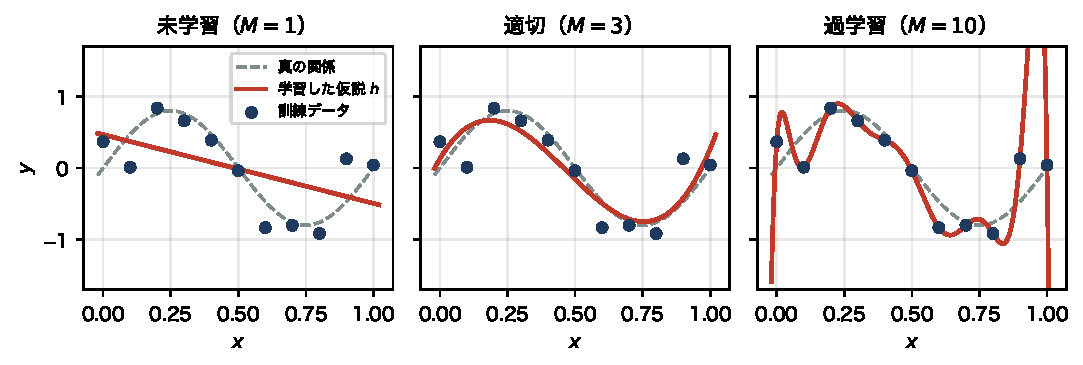
\includegraphics[width=1.0\linewidth]{figures/ch1_fit}
  \caption{同じ訓練データに対する3つの仮説。仮説空間が小さすぎると構造を捉えられず（左）、大きすぎるとノイズまで再現してしまう（右）。}
  \label{fig:fit}
\end{figure}

\begin{figure}[H]
  \centering
  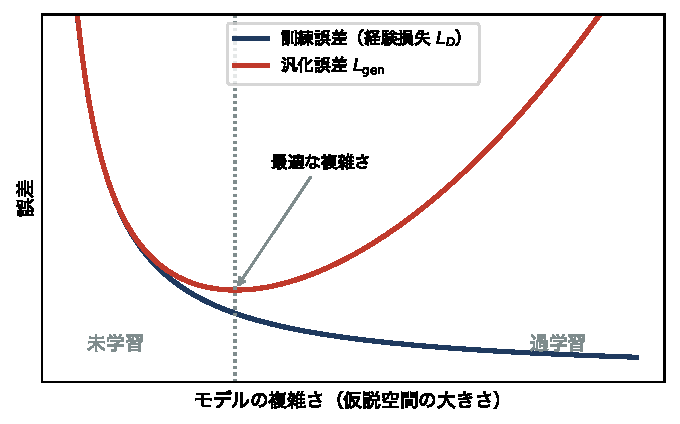
\includegraphics[width=0.62\linewidth]{figures/ch1_error_curve}
  \caption{モデルの複雑さと2つの誤差。訓練誤差は単調に減少するが、汎化誤差はある点を境に増加に転じる。}
  \label{fig:errorcurve}
\end{figure}

適切な仮説空間の選択、すなわちモデルの複雑さの制御は、
機械学習における中心的な課題であり、第6回で扱う\textbf{正則化}によって対処する。


\subsection{学習アルゴリズムの概要}

以上をまとめると、機械学習の基本的な枠組みは次の3ステップからなる：

\begin{enumerate}
  \item \textbf{仮説空間の設定}: モデルの形（線形、多項式、ニューラルネットワークなど）を決める。
  \item \textbf{損失関数の選択}: 予測の良さの評価基準を定める。
  \item \textbf{最適化}: 訓練データに対する経験損失を最小化する仮説 $h^*$ を求める：
    \begin{equation}
      h^* = \arg\min_{h \in \mathcal{H}} L_D(h)
    \end{equation}
    右辺の $\arg\min_{h \in \mathcal{H}} L_D(h)$ は
    「$\mathcal{H}$ に属する $h$ のうち $L_D(h)$ を最小にするもの」を表す。
    $\min_{h} L_D(h)$ が最小値（損失の値そのもの）を指すのに対し、
    $\arg\min_{h} L_D(h)$ はその最小値を達成する $h$（引数）を指す点に注意する。
    上付きの $*$ は、この最小化問題の解、すなわち最適解であることを示す。
    パラメトリックモデルでは、これはパラメータの最適化に帰着する：
    \begin{equation}
      \bm{w}^* = \arg\min_{\bm{w} \in \mathbb{R}^p}
      \frac{1}{N} \sum_{i=1}^{N} L(y_i, h(\bm{x}_i; \bm{w}))
    \end{equation}
    $\bm{w}^*$ は経験損失を最小にする最適なパラメータであり、
    $h^* = h(\cdot; \bm{w}^*)$ という関係にある。
\end{enumerate}

第4回・第5回では、この最適化問題を具体的に解く方法（正規方程式と勾配降下法）を学ぶ。

なお、本章では学習を「経験損失の最小化」として定式化した。
この枠組みは明快であるが、過学習の問題に対して本質的な解決を与えない。
第7回以降では、確率論とベイズの定理に基づく別の視点から学習を捉え直し、
正則化がなぜ有効なのかを数理的に明らかにする。


\subsection{演習問題}

\begin{enumerate}
  \item \textbf{記法の確認}\quad
    次の各主張が正しいか否かを判定し、その理由を述べよ。
    \begin{enumerate}
      \item $\bm{x} \in \mathbb{R}^3$ かつ $\mathcal{X} \subseteq \mathbb{R}^3$ であれば、
        常に $\bm{x} \in \mathcal{X}$ が成り立つ。
      \item $h : \mathbb{R}^2 \to \{0, 1\}$ は、2次元入力に対する2値分類の仮説を表す。
      \item $\mathcal{Y} = \{0, 1\}$ のとき、直積 $\mathcal{Y} \times \mathcal{Y}$ の要素の個数は $4$ である。
      \item $h(\cdot\,; \bm{w})$ と $h(\bm{x}; \bm{w})$ は、どちらも関数そのものを指す記法である。
    \end{enumerate}

  \item \textbf{パラメータ次元}\quad
    次の各仮説空間のパラメータ次元 $p$ を求めよ。
    \begin{enumerate}
      \item 入力 $\bm{x} \in \mathbb{R}^5$ に対する線形モデル $h(\bm{x}; \bm{w}) = w_0 + \bm{w}_{1:5}^\top \bm{x}$
      \item 入力 $x \in \mathbb{R}$ に対する3次多項式モデル
      \item 入力 $\bm{x} = (x_1, x_2)^\top \in \mathbb{R}^2$ に対して、
        2次以下のすべての単項式 $1, x_1, x_2, x_1^2, x_1 x_2, x_2^2$ の線形結合で表されるモデル
    \end{enumerate}

  \item \textbf{仮説空間の包含関係}\quad
    $\mathcal{H}_M$ を $M$ 次多項式仮説空間とする。
    $\mathcal{H}_1 \subset \mathcal{H}_2$（$\mathcal{H}_1$ は $\mathcal{H}_2$ の真部分集合）であることを、
    次の2点を示すことで証明せよ。
    \begin{enumerate}
      \item 任意の $h \in \mathcal{H}_1$ は $\mathcal{H}_2$ の要素でもある。
      \item $\mathcal{H}_2$ の要素であって $\mathcal{H}_1$ の要素ではない関数が存在する。
    \end{enumerate}

  \item \textbf{経験損失の計算}\quad
    訓練データ $D = \{(1, 3),\; (2, 5),\; (3, 6)\}$ が与えられている
    （各組は $(x_i, y_i)$ を表す）。
    2つの仮説
    \begin{equation*}
      h_a(x) = 2x + 1, \qquad h_b(x) = 1.5x + 1.5
    \end{equation*}
    について、二乗損失に基づく経験損失 $L_D(h_a)$, $L_D(h_b)$ をそれぞれ計算し、
    どちらの仮説が訓練データに対して良いかを判定せよ。

  \item \textbf{0-1損失}\quad
    5個の訓練データに対する真のラベルと仮説 $h$ の予測が次のように与えられている。
    \begin{center}
      \begin{tabular}{c|ccccc}
        $i$ & 1 & 2 & 3 & 4 & 5 \\
        \hline
        $y_i$ & 1 & 0 & 1 & 1 & 0 \\
        $h(\bm{x}_i)$ & 1 & 0 & 0 & 1 & 1 \\
      \end{tabular}
    \end{center}
    0-1損失に基づく経験損失 $L_D(h)$ を求めよ。
    また、この値が一般に何と呼ばれる量に一致するかを述べよ。

  \item \textbf{$\min$ と $\arg\min$}\quad
    問4の設定で、仮説空間を $\mathcal{H} = \{h_a, h_b\}$ の2要素からなる集合とする。
    このとき
    \begin{equation*}
      \min_{h \in \mathcal{H}} L_D(h), \qquad h^* = \arg\min_{h \in \mathcal{H}} L_D(h)
    \end{equation*}
    をそれぞれ求めよ。両者の違いを一言で説明せよ。

  \item \textbf{経験損失と汎化誤差}\quad
    平面上の3点 $(x_1, y_1), (x_2, y_2), (x_3, y_3)$（$x_i$ は互いに異なる）が与えられたとき、
    これらをすべて通る2次多項式 $h \in \mathcal{H}_2$ がただ一つ存在する。
    \begin{enumerate}
      \item この $h$ の二乗損失に基づく経験損失 $L_D(h)$ を求めよ。
      \item この $h$ の汎化誤差 $L_{\mathrm{gen}}(h)$ も $0$ であると言えるか。
        理由とともに述べよ。
      \item 一般に $N$ 個のデータ点（$x_i$ は互いに異なる）が与えられたとき、
        経験損失を $0$ にできる多項式の次数 $M$ の最小値はいくらか。
        この事実と過学習の関係を説明せよ。
    \end{enumerate}

\end{enumerate}




\pagebreak

%===========================================
% Chapter 2
%===========================================
\section{ベクトルと内積}

第1回では、入力を $\bm{x} \in \mathbb{R}^d$ というベクトルで表し、
線形モデルを $h(\bm{x}; \bm{w}) = w_0 + \bm{w}_{1:d}^\top \bm{x}$ と書いた。
本章では、この $\bm{w}_{1:d}^\top \bm{x}$ という演算、すなわち\textbf{内積}の意味を明らかにする。
内積は単なる計算規則ではなく、「長さ」と「角度」という幾何学的な情報を担っており、
機械学習において\textbf{類似度}を測る基本的な道具となる。
本章の最後では、現代AIの2つの柱である Transformer の Attention 機構と
ニューラルネットワークが、いずれも内積によって構成されていることを見る。


\subsection{ベクトルとは何か}

\subsubsection{データの表現としてのベクトル}

$d$ 個の実数を順番に並べたものを $d$ 次元\textbf{ベクトル}（vector）と呼び、
本書では太字の小文字で表す：
\begin{equation}
  \bm{x} = (x_1, x_2, \ldots, x_d)^\top \in \mathbb{R}^d
\end{equation}
ここで $x_i$ を第 $i$ \textbf{成分}（component）と呼ぶ。
右肩の $\top$ は\textbf{転置}（transpose）を表す記号であり、
横に並べた表記を縦に並べ替えることを意味する：
\begin{equation}
  (x_1, x_2, \ldots, x_d)^\top =
  \begin{pmatrix} x_1 \\ x_2 \\ \vdots \\ x_d \end{pmatrix}
\end{equation}
本書ではベクトルを\textbf{列ベクトル}（縦に並べたもの）として扱う。
文章中では紙面の都合で横に書き、転置の記号を付けて列ベクトルであることを示す。

第1回の例2では、部屋の広さ $x_1$ と駅からの距離 $x_2$ を
$\bm{x} = (x_1, x_2)^\top \in \mathbb{R}^2$ と表した。
このように、機械学習ではデータの複数の属性（特徴量）を並べてベクトルとする。
$d$ 次元のベクトルは、$d$ 個の特徴で記述されたデータ1件に対応する。

\subsubsection{ベクトルの演算}

2つのベクトル $\bm{x}, \bm{y} \in \mathbb{R}^d$ と実数 $c \in \mathbb{R}$ に対して、
\textbf{和}と\textbf{スカラー倍}を成分ごとに定める：
\begin{align}
  \bm{x} + \bm{y} &= (x_1 + y_1,\; x_2 + y_2,\; \ldots,\; x_d + y_d)^\top \\
  c\bm{x} &= (c x_1,\; c x_2,\; \ldots,\; c x_d)^\top
\end{align}
ここで $c$ のような1個の実数を、ベクトルと区別して\textbf{スカラー}（scalar）と呼ぶ。

幾何学的には、ベクトルは原点から点 $(x_1, \ldots, x_d)$ に向かう矢印と見なせる。
和は矢印をつなげた結果（平行四辺形の対角線）であり、
スカラー倍は矢印を $c$ 倍に伸縮する操作である（$c < 0$ なら向きが反転する）。


\begin{figure}[H]
  \centering
  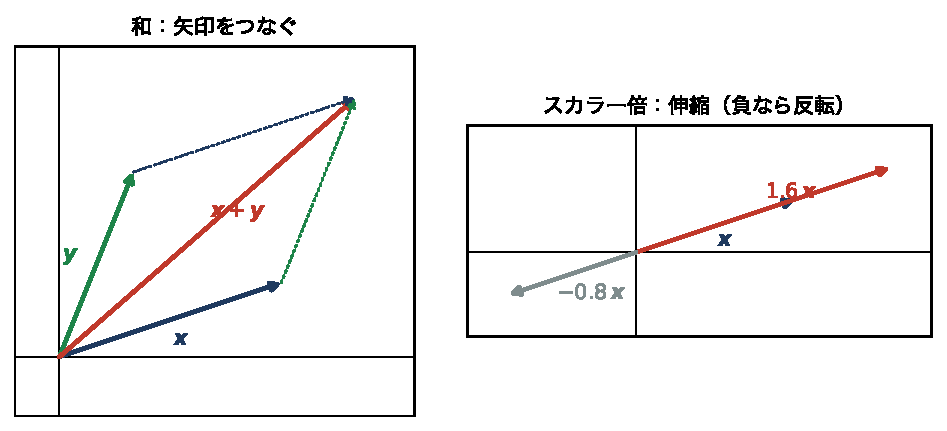
\includegraphics[width=0.92\linewidth]{figures/ch2_vec_ops}
  \caption{ベクトルの和とスカラー倍の幾何学的な意味。}
  \label{fig:vecops}
\end{figure}

なお、成分がすべて $0$ のベクトルを\textbf{零ベクトル}（zero vector）と呼び、$\bm{0}$ と書く。


\subsection{ノルム}

\subsubsection{ベクトルの長さ}

ベクトルの「長さ」を測る量を\textbf{ノルム}（norm）と呼ぶ。
2次元の場合、$\bm{x} = (x_1, x_2)^\top$ の長さは三平方の定理より
$\sqrt{x_1^2 + x_2^2}$ である。これを一般の次元に拡張する。

\begin{itembox}[l]{定義：ユークリッドノルム}
ベクトル $\bm{x} = (x_1, \ldots, x_d)^\top \in \mathbb{R}^d$ に対して、
\begin{equation}
  \|\bm{x}\| = \sqrt{x_1^2 + x_2^2 + \cdots + x_d^2} = \sqrt{\sum_{i=1}^{d} x_i^2}
\end{equation}
を $\bm{x}$ の\textbf{ユークリッドノルム}（Euclidean norm）または $L^2$ ノルムと呼ぶ。
記号 $\|\bm{x}\|$ は「$\bm{x}$ のノルム」と読む。
\end{itembox}

絶対値の記号 $|x|$ が実数の大きさを表すのに対し、
二重線の記号 $\|\bm{x}\|$ はベクトルの大きさを表す。
$d = 1$ のとき $\|\bm{x}\| = \sqrt{x_1^2} = |x_1|$ となり、絶対値と一致する。

例えば $\bm{x} = (3, 4)^\top$ のとき
\begin{equation*}
  \|\bm{x}\| = \sqrt{3^2 + 4^2} = \sqrt{25} = 5
\end{equation*}
である。

\subsubsection{ノルムの性質}

ノルムは次の3つの性質をもつ。これらは「長さ」という概念が満たすべき自然な要請である。

\begin{itembox}[l]{定理：ノルムの基本性質}
任意の $\bm{x}, \bm{y} \in \mathbb{R}^d$、$c \in \mathbb{R}$ に対して、
\begin{align}
  &\|\bm{x}\| \geq 0, \quad \text{かつ} \quad \|\bm{x}\| = 0 \iff \bm{x} = \bm{0}
    &&\text{（非負性）} \\
  &\|c\bm{x}\| = |c| \, \|\bm{x}\|
    &&\text{（斉次性）} \\
  &\|\bm{x} + \bm{y}\| \leq \|\bm{x}\| + \|\bm{y}\|
    &&\text{（三角不等式）}
\end{align}
\end{itembox}

記号 $\iff$ は「必要十分条件である」「同値である」と読む。
また、3つの性質の名称の読みと意味は次のとおりである。

\begin{center}
\begin{tabular}{l|l|l|p{6.0cm}}
\hline
名称 & 読み & 英語 & 意味 \\
\hline\hline
非負性 & ひふせい & nonnegativity & 長さは負にならない。長さが $0$ なのは零ベクトルだけ \\
斉次性 & せいじせい & homogeneity & ベクトルを $c$ 倍すると長さも $|c|$ 倍になる（比例する） \\
三角不等式 & さんかくふとうしき & triangle inequality & 遠回りは近道より長い \\
\hline
\end{tabular}
\end{center}

\textbf{斉次}（homogeneous、せいじ）とは「等しく揃っている」という意味の語で、
数学では「入力を定数倍すると、出力もそれに応じて一定の規則で定数倍される」性質を指す。
ノルムの場合、$\|c\bm{x}\| = |c|\,\|\bm{x}\|$ は
「矢印を2倍に伸ばせば長さも2倍、$3$ 倍に伸ばせば長さも $3$ 倍になる」ことを述べている。
絶対値が付くのは、$c$ が負のときは向きが反転するだけで長さは正のまま
（$c = -2$ なら長さは $2$ 倍）だからである。
この性質があるおかげで、第2.2.3項で述べる\textbf{正規化}
$\bm{u} = \bm{x}/\|\bm{x}\|$ が $\|\bm{u}\| = 1$ を与えることが保証される。実際、
\begin{equation}
  \left\| \frac{\bm{x}}{\|\bm{x}\|} \right\|
  = \left\| \frac{1}{\|\bm{x}\|} \bm{x} \right\|
  = \frac{1}{\|\bm{x}\|} \, \|\bm{x}\| = 1
\end{equation}
であり、ここで斉次性を用いている。

非負性と斉次性は定義から直ちに従う。実際、斉次性は
\begin{equation}
  \|c\bm{x}\| = \sqrt{\sum_{i=1}^{d} (c x_i)^2} = \sqrt{c^2 \sum_{i=1}^{d} x_i^2}
  = |c| \sqrt{\sum_{i=1}^{d} x_i^2} = |c| \, \|\bm{x}\|
\end{equation}
と示される。ここで $\sqrt{c^2} = |c|$ であり、$c$ そのものではないことに注意する。
三角不等式は「遠回りは近道より長い」という主張である。
$\bm{x}$ だけ進んでから $\bm{y}$ だけ進む道のり $\|\bm{x}\| + \|\bm{y}\|$ は、
直接 $\bm{x} + \bm{y}$ だけ進む道のり $\|\bm{x} + \bm{y}\|$ 以上である、ということを述べている。
これは第2.4.1項で述べるコーシー・シュワルツの不等式から導かれる。
証明の方針は、両辺が非負であることに注意して\textbf{両辺を二乗して比較する}ことである。
左辺の二乗を内積の性質で展開し、現れた項にコーシー・シュワルツの不等式を適用すればよい。
実際の証明は演習問題4で扱う。

\subsubsection{距離と単位ベクトル}

2つのベクトルの「離れ具合」は、差のノルムで測る：
\begin{equation}
  \mathrm{dist}(\bm{x}, \bm{y}) = \|\bm{x} - \bm{y}\|
  = \sqrt{\sum_{i=1}^{d} (x_i - y_i)^2}
\end{equation}
これを\textbf{ユークリッド距離}（Euclidean distance）と呼ぶ。

第1回で導入した二乗損失 $L(y, h(\bm{x})) = (y - h(\bm{x}))^2$ を
$N$ 個のデータについて足し合わせたものは、
真の値を並べたベクトル $\bm{y} = (y_1, \ldots, y_N)^\top$ と
予測を並べたベクトル $\hat{\bm{y}} = (h(\bm{x}_1), \ldots, h(\bm{x}_N))^\top$ を用いて
\begin{equation}
  \sum_{i=1}^{N} (y_i - h(\bm{x}_i))^2 = \|\bm{y} - \hat{\bm{y}}\|^2
\end{equation}
と書ける。すなわち\textbf{経験損失の最小化とは、距離の最小化である}。
この見方は第4回で最小二乗法を「射影」として理解する際の出発点となる。

また、ノルムが $1$ のベクトルを\textbf{単位ベクトル}（unit vector）と呼ぶ。
$\bm{x} \neq \bm{0}$ に対して
\begin{equation}
  \bm{u} = \frac{\bm{x}}{\|\bm{x}\|}
\end{equation}
とすれば $\|\bm{u}\| = 1$ となる。この操作を\textbf{正規化}（normalization）と呼び、
「長さの情報を捨てて向きだけを取り出す」ことに対応する。


\subsection{内積}

\subsubsection{内積の定義}

\begin{itembox}[l]{定義：内積}
2つのベクトル $\bm{x} = (x_1, \ldots, x_d)^\top$、$\bm{y} = (y_1, \ldots, y_d)^\top \in \mathbb{R}^d$
に対して、
\begin{equation}
  \bm{x}^\top \bm{y} = x_1 y_1 + x_2 y_2 + \cdots + x_d y_d = \sum_{i=1}^{d} x_i y_i
\end{equation}
を $\bm{x}$ と $\bm{y}$ の\textbf{内積}（inner product）と呼ぶ。
内積の値は\textbf{スカラー}（1個の実数）である。
\end{itembox}

内積は $\langle \bm{x}, \bm{y} \rangle$ や $\bm{x} \cdot \bm{y}$ とも書かれるが、
本書では行列との統一のため $\bm{x}^\top \bm{y}$ という記法を用いる。
「エックスの転置 ワイ」と読む。

例えば $\bm{x} = (1, 2, 3)^\top$、$\bm{y} = (4, 5, 6)^\top$ のとき
\begin{equation*}
  \bm{x}^\top \bm{y} = 1 \times 4 + 2 \times 5 + 3 \times 6 = 4 + 10 + 18 = 32
\end{equation*}
である。

ノルムと内積の間には、定義から直ちに次の関係が成り立つ：
\begin{equation}
  \bm{x}^\top \bm{x} = \sum_{i=1}^{d} x_i^2 = \|\bm{x}\|^2,
  \qquad \text{すなわち} \quad \|\bm{x}\| = \sqrt{\bm{x}^\top \bm{x}}
\end{equation}
つまり、ノルムは内積から定まる量である。

\subsubsection{内積の性質}

\begin{itembox}[l]{定理：内積の基本性質}
任意の $\bm{x}, \bm{y}, \bm{z} \in \mathbb{R}^d$、$c \in \mathbb{R}$ に対して、
\begin{align}
  &\bm{x}^\top \bm{y} = \bm{y}^\top \bm{x} &&\text{（対称性）} \\
  &(\bm{x} + \bm{y})^\top \bm{z} = \bm{x}^\top \bm{z} + \bm{y}^\top \bm{z} &&\text{（加法性）} \\
  &(c\bm{x})^\top \bm{y} = c\, (\bm{x}^\top \bm{y}) &&\text{（斉次性）} \\
  &\bm{x}^\top \bm{x} \geq 0, \quad \text{かつ} \quad \bm{x}^\top \bm{x} = 0 \iff \bm{x} = \bm{0}
    &&\text{（正定値性）}
\end{align}
加法性と斉次性をあわせて\textbf{線形性}（linearity）と呼ぶ。
\end{itembox}

4つの性質の読みと意味は次のとおりである。

\begin{center}
\begin{tabular}{l|l|l|p{5.6cm}}
\hline
名称 & 読み & 英語 & 意味 \\
\hline\hline
対称性 & たいしょうせい & symmetry & 掛ける順序を入れ替えても値が変わらない \\
加法性 & かほうせい & additivity & 和の内積は、内積の和に分解できる \\
斉次性 & せいじせい & homogeneity & 片方を $c$ 倍すると、内積も $c$ 倍になる \\
正定値性 & せいていちせい & positive & 自分自身との内積は負にならず、 \\
 & & definiteness & $0$ になるのは零ベクトルのときだけ \\
\hline
\end{tabular}
\end{center}

ノルムの斉次性では絶対値 $|c|$ が付いたのに対し、
内積の斉次性では $c$ がそのまま出てくる点に注意する。
長さは常に正であるのに対し、内積は負の値も取りうるからである。

加法性と斉次性をあわせた\textbf{線形性}は、
「$\bm{x}$ を動かしたときに $\bm{x}^\top \bm{y}$ がどう変わるか」を表している。
2つを一つの式にまとめると、任意の $a, b \in \mathbb{R}$ に対して
\begin{equation}
  (a\bm{x} + b\bm{y})^\top \bm{z} = a\,(\bm{x}^\top \bm{z}) + b\,(\bm{y}^\top \bm{z})
\end{equation}
すなわち\textbf{線形結合の内積は、内積の線形結合になる}。
この性質は本書で繰り返し用いられる。
例えば後述するコーシー・シュワルツの不等式の証明では、
$\|\bm{x} - t\bm{y}\|^2$ を展開する際にこの線形性を使っている。

\textbf{正定値性}（positive definiteness）は、ノルムの非負性に対応する性質である。
$\bm{x}^\top \bm{x} = \|\bm{x}\|^2$ であったから、
「自分自身との内積が $0$ になるのは零ベクトルだけ」という主張は
「長さが $0$ のベクトルは零ベクトルだけ」と同じことを述べている。

なお、\textbf{正定値性は内積に限られた概念ではない}。
一般に「ある量が常に $0$ 以上であり、$0$ になるのは自明な場合だけである」
という形の性質を、広く\textbf{正定値}（positive definite）と呼ぶ。
本講義で登場するものを挙げておく。

\begin{center}
\begin{tabular}{l|l|l}
\hline
対象 & 正定値の条件 & 登場する回 \\
\hline\hline
内積 & $\bm{x}^\top \bm{x} > 0 \;\; (\bm{x} \neq \bm{0})$ & 第2回（本章） \\
行列 $\bm{A}$ & $\bm{x}^\top \bm{A} \bm{x} > 0 \;\; (\bm{x} \neq \bm{0})$ & 第3回、第5回 \\
カーネル $k$ & $\sum_{i,j} c_i c_j\, k(\bm{x}_i, \bm{x}_j) > 0$ & 第11回 \\
\hline
\end{tabular}
\end{center}

内積の正定値性は、$\bm{A}$ を単位行列とした場合の特別な場合にあたる。

ここで、よく似た用語である\textbf{半正定値}（positive semi-definite）との違いに注意する。
等号が成り立つ場合を許すかどうかが両者を分ける。
\begin{align}
  \text{正定値：} \quad & \bm{x}^\top \bm{A}\bm{x} > 0 \quad (\text{すべての } \bm{x} \neq \bm{0}) \\
  \text{半正定値：} \quad & \bm{x}^\top \bm{A}\bm{x} \geq 0 \quad (\text{すべての } \bm{x})
\end{align}
半正定値では、$\bm{x} \neq \bm{0}$ でありながら $\bm{x}^\top \bm{A}\bm{x} = 0$ となる
「つぶれた方向」が存在しうる。
この違いは後の回で本質的な意味をもつ。
例えば第3回で扱う計画行列 $\bm{X}$ に対して $\bm{X}^\top \bm{X}$ は常に半正定値であるが、
正定値になるのは $\bm{X}$ がフルランクのとき、すなわち多重共線性がないときに限る。
つぶれた方向の存在が、最適なパラメータが一意に定まらないことに対応している。

また、第5回で扱う\textbf{凸関数}の判定でもこの語が現れる。
関数の曲がり具合を表す行列（ヘッセ行列）が
半正定値であれば凸、正定値であれば狭義凸（最小値を与える点がただ一つ）となる。
これも「つぶれた方向があるかどうか」の違いである。

以下、これらの性質を証明する。
なお本書では、証明の終わりを記号 $\blacksquare$ で示す。
これは「証明終わり」を意味する慣習的な記号であり、
\textbf{墓石記号}（tombstone）またはハルモス記号（Halmos symbol）と呼ばれる。
ラテン語の \textit{quod erat demonstrandum}（「これが示すべきことであった」）を略した
\textbf{Q.E.D.} が同じ意味で用いられることもある。

\noindent
\textbf{証明}\quad
対称性は、実数の積が可換（$x_i y_i = y_i x_i$）であることから
\begin{equation}
  \bm{x}^\top \bm{y} = \sum_{i=1}^{d} x_i y_i = \sum_{i=1}^{d} y_i x_i = \bm{y}^\top \bm{x}
\end{equation}
加法性は、和の定義と総和の分配より
\begin{equation}
  (\bm{x} + \bm{y})^\top \bm{z} = \sum_{i=1}^{d} (x_i + y_i) z_i
  = \sum_{i=1}^{d} x_i z_i + \sum_{i=1}^{d} y_i z_i
  = \bm{x}^\top \bm{z} + \bm{y}^\top \bm{z}
\end{equation}
斉次性も同様に
\begin{equation}
  (c\bm{x})^\top \bm{y} = \sum_{i=1}^{d} (c x_i) y_i = c \sum_{i=1}^{d} x_i y_i = c\,(\bm{x}^\top \bm{y})
\end{equation}
正定値性は $\bm{x}^\top \bm{x} = \sum_i x_i^2$ が二乗和であることから従う。
二乗和が $0$ になるのは、すべての項が $0$ のとき、すなわち $\bm{x} = \bm{0}$ のときに限る。
\hfill $\blacksquare$

\subsubsection{線形モデルの再解釈}

内積の記法を用いると、第1回の線形モデルは
\begin{equation}
  h(\bm{x}; \bm{w}) = w_0 + \bm{w}_{1:d}^\top \bm{x}
\end{equation}
と書けた。さらに、入力に定数 $1$ を付け加えて
$\tilde{\bm{x}} = (1, x_1, \ldots, x_d)^\top \in \mathbb{R}^{d+1}$ とすれば、
\begin{equation}
  h(\bm{x}; \bm{w}) = \bm{w}^\top \tilde{\bm{x}}, \qquad \bm{w} = (w_0, w_1, \ldots, w_d)^\top
\end{equation}
と、バイアス項も含めて一つの内積で表せる。
この $1$ を加える操作を\textbf{バイアス項の吸収}と呼び、以降の式変形を簡潔にする。

すなわち\textbf{線形モデルとは、入力ベクトルとパラメータベクトルの内積である}。
第4回以降で扱う最小二乗法、第10回のサポートベクターマシン、
第12回のニューラルネットワークは、いずれもこの内積を基本要素として構成される。


\subsection{内積の幾何学的解釈}

\subsubsection{コーシー・シュワルツの不等式}

内積が「角度」を表すことを見るために、まず次の不等式を示す。

\begin{itembox}[l]{定理：コーシー・シュワルツの不等式}
任意の $\bm{x}, \bm{y} \in \mathbb{R}^d$ に対して、
\begin{equation}
  |\bm{x}^\top \bm{y}| \leq \|\bm{x}\| \, \|\bm{y}\|
\end{equation}
等号が成立するのは、$\bm{x}$ と $\bm{y}$ が平行なとき、
すなわち一方が他方のスカラー倍であるときに限る。
\end{itembox}

\noindent
\textbf{証明}\quad
まず $\bm{y} = \bm{0}$ の場合を除いておく。このとき左辺は $|\bm{x}^\top \bm{0}| = 0$、
右辺は $\|\bm{x}\| \cdot 0 = 0$ であり、等号が成立する。以下 $\bm{y} \neq \bm{0}$ とする。

任意の実数 $t$ に対して次の関数を考える：
\begin{equation}
  f(t) = \|\bm{x} - t\bm{y}\|^2
\end{equation}
ノルムの二乗は非負なので、\textbf{すべての $t$ に対して} $f(t) \geq 0$ である。
一方、内積の性質を用いて $f(t)$ を展開すると
\begin{align}
  f(t) &= (\bm{x} - t\bm{y})^\top (\bm{x} - t\bm{y}) \notag \\
       &= \bm{x}^\top \bm{x} - t\, \bm{x}^\top \bm{y} - t\, \bm{y}^\top \bm{x} + t^2 \bm{y}^\top \bm{y} \notag \\
       &= \|\bm{y}\|^2 t^2 - 2 (\bm{x}^\top \bm{y}) t + \|\bm{x}\|^2
  \label{eq:cs-quadratic}
\end{align}
となる（対称性 $\bm{x}^\top \bm{y} = \bm{y}^\top \bm{x}$ を用いた）。
これは $t$ についての2次関数であり、$\bm{y} \neq \bm{0}$ より
2次の係数 $\|\bm{y}\|^2$ は正である。

\paragraph{不等式の証明}
2次関数 $f(t) = at^2 + bt + c$（$a > 0$）について、
\begin{equation}
  \text{すべての } t \text{ で } f(t) \geq 0
  \quad \Longleftrightarrow \quad
  \text{判別式 } D = b^2 - 4ac \leq 0
\end{equation}
が成り立つ。実際、平方完成すると
\begin{equation}
  f(t) = a\left( t + \frac{b}{2a} \right)^2 - \frac{D}{4a}
\end{equation}
であり、$t = -b/(2a)$ のとき最小値 $-D/(4a)$ をとる。
$a > 0$ であるから、この最小値が $0$ 以上であることと $D \leq 0$ は同値である。

式\eqref{eq:cs-quadratic}に適用すると
$a = \|\bm{y}\|^2$、$b = -2(\bm{x}^\top \bm{y})$、$c = \|\bm{x}\|^2$ なので、
\begin{equation}
  \frac{D}{4} = (\bm{x}^\top \bm{y})^2 - \|\bm{y}\|^2 \|\bm{x}\|^2 \leq 0
  \label{eq:cs-disc}
\end{equation}
すなわち $(\bm{x}^\top \bm{y})^2 \leq \|\bm{x}\|^2 \|\bm{y}\|^2$ を得る。
両辺は非負なので平方根をとってよく、
$|\bm{x}^\top \bm{y}| \leq \|\bm{x}\| \, \|\bm{y}\|$ が示された。

\paragraph{等号成立条件の証明}
「$\bm{x}$ と $\bm{y}$ が平行」を「一方が他方のスカラー倍である」の意味で用いる。
必要性と十分性を順に示す。

\textbf{(i) 等号が成立するならば平行である。}\quad
等号 $|\bm{x}^\top \bm{y}| = \|\bm{x}\| \|\bm{y}\|$ が成り立つとする。
両辺は非負なので、二乗しても同値であり
\begin{equation}
  (\bm{x}^\top \bm{y})^2 = \|\bm{x}\|^2 \|\bm{y}\|^2
  \label{eq:cs-eq}
\end{equation}
が成り立つ。

ここで、$f$ が最小値をとる $t$ の値を $t_0$ とおく。
平方完成の式 $f(t) = a(t + \frac{b}{2a})^2 - \frac{D}{4a}$ より $t_0 = -b/(2a)$ であり、
$a = \|\bm{y}\|^2$、$b = -2(\bm{x}^\top \bm{y})$ を代入すると
\begin{equation}
  t_0 = -\frac{b}{2a} = -\frac{-2(\bm{x}^\top \bm{y})}{2\|\bm{y}\|^2}
      = \frac{\bm{x}^\top \bm{y}}{\|\bm{y}\|^2}
\end{equation}
となる。この $t_0$ における $f$ の値を、式\eqref{eq:cs-quadratic}に代入して直接計算する：
\begin{align}
  f(t_0) &= \|\bm{y}\|^2 t_0^2 - 2(\bm{x}^\top \bm{y})\, t_0 + \|\bm{x}\|^2 \notag \\
         &= \|\bm{y}\|^2 \cdot \frac{(\bm{x}^\top \bm{y})^2}{\|\bm{y}\|^4}
            - 2(\bm{x}^\top \bm{y}) \cdot \frac{\bm{x}^\top \bm{y}}{\|\bm{y}\|^2} + \|\bm{x}\|^2 \notag \\
         &= \frac{(\bm{x}^\top \bm{y})^2}{\|\bm{y}\|^2}
            - \frac{2(\bm{x}^\top \bm{y})^2}{\|\bm{y}\|^2} + \|\bm{x}\|^2 \notag \\
         &= \|\bm{x}\|^2 - \frac{(\bm{x}^\top \bm{y})^2}{\|\bm{y}\|^2}
          = \frac{\|\bm{x}\|^2 \|\bm{y}\|^2 - (\bm{x}^\top \bm{y})^2}{\|\bm{y}\|^2}
\end{align}
ここで、仮定した等式\eqref{eq:cs-eq}より最後の分子は $0$ である。よって
\begin{equation}
  f(t_0) = 0
  \label{eq:cs-ft0}
\end{equation}
が得られる。

一方、$f$ はそもそも $f(t) = \|\bm{x} - t\bm{y}\|^2$ と定義したものであったから、
$t = t_0$ を代入して
\begin{equation}
  f(t_0) = \|\bm{x} - t_0 \bm{y}\|^2
  \label{eq:cs-ft0-def}
\end{equation}
でもある。式\eqref{eq:cs-ft0}と式\eqref{eq:cs-ft0-def}を見比べると
\begin{equation}
  \|\bm{x} - t_0 \bm{y}\|^2 = 0
\end{equation}
を得る。ノルムの非負性より $\|\bm{v}\| = 0 \iff \bm{v} = \bm{0}$ であったから、
$\bm{x} - t_0\bm{y} = \bm{0}$、すなわち
\begin{equation}
  \bm{x} = t_0 \bm{y} = \frac{\bm{x}^\top \bm{y}}{\|\bm{y}\|^2} \, \bm{y}
\end{equation}
となり、$\bm{x}$ は $\bm{y}$ のスカラー倍、すなわち両者は平行である。

\textbf{(ii) 平行ならば等号が成立する。}\quad
逆に $\bm{x} = c\,\bm{y}$（$c \in \mathbb{R}$）と書けるとする。
内積とノルムの斉次性を用いると
\begin{equation}
  |\bm{x}^\top \bm{y}| = |(c\bm{y})^\top \bm{y}| = |c| \, \|\bm{y}\|^2, \qquad
  \|\bm{x}\| \, \|\bm{y}\| = \|c\bm{y}\| \, \|\bm{y}\| = |c| \, \|\bm{y}\|^2
\end{equation}
となり、両者は一致する。よって等号が成立する。

(i) と (ii) より、等号が成立することと $\bm{x}, \bm{y}$ が平行であることは同値である。
なお、最初に除いた $\bm{y} = \bm{0}$ の場合も、$\bm{y} = 0 \cdot \bm{x}$ と書けるので
「平行かつ等号成立」であり、この主張に含まれる。
\hfill $\blacksquare$

\subsubsection{内積と角度}

前項で証明したコーシー・シュワルツの不等式
$|\bm{x}^\top \bm{y}| \leq \|\bm{x}\| \, \|\bm{y}\|$ から、次のことがわかる。

$\bm{x}, \bm{y} \neq \bm{0}$ とすると、ノルムの非負性より $\|\bm{x}\| > 0$、$\|\bm{y}\| > 0$ であり、
その積 $\|\bm{x}\| \, \|\bm{y}\|$ は正である。
正の数で不等式の両辺を割っても向きは変わらないので、
\begin{equation}
  \frac{|\bm{x}^\top \bm{y}|}{\|\bm{x}\| \, \|\bm{y}\|} \leq 1
\end{equation}
を得る。ここで $|a|/b = |a/b|$（$b > 0$）であるから、左辺は
$\left| \dfrac{\bm{x}^\top \bm{y}}{\|\bm{x}\| \, \|\bm{y}\|} \right|$ と書ける。
一般に実数 $u$ について $|u| \leq 1$ と $-1 \leq u \leq 1$ は同値であるから、
\begin{equation}
  -1 \leq \frac{\bm{x}^\top \bm{y}}{\|\bm{x}\| \, \|\bm{y}\|} \leq 1
  \label{eq:cos-range}
\end{equation}
が成り立つ。

この値の範囲 $[-1, 1]$ は、余弦関数 $\cos$ の値域と一致する。
すなわち、式\eqref{eq:cos-range}の中央の量に対して、
それを $\cos\theta$ とするような角 $\theta$ が必ず存在する
（$0 \leq \theta \leq \pi$ の範囲では $\cos$ は単調減少で、値域が $[-1,1]$ であるから、
そのような $\theta$ はただ一つに定まる）。そこで次のように定義する。

\begin{itembox}[l]{定義：なす角}
$\bm{x}, \bm{y} \neq \bm{0}$ に対して、
\begin{equation}
  \cos\theta = \frac{\bm{x}^\top \bm{y}}{\|\bm{x}\| \, \|\bm{y}\|},
  \qquad 0 \leq \theta \leq \pi
\end{equation}
を満たす $\theta$ を、$\bm{x}$ と $\bm{y}$ の\textbf{なす角}と呼ぶ。
変形すれば、内積は次のように表される：
\begin{equation}
  \bm{x}^\top \bm{y} = \|\bm{x}\| \, \|\bm{y}\| \cos\theta
\end{equation}
\end{itembox}

この式が本章の中心である。内積は
\textbf{「2つのベクトルの長さの積」×「向きの一致度」}という構造をもつ。

\begin{itemize}
  \item $\theta = 0$（同じ向き）のとき $\cos\theta = 1$ で、内積は最大値 $\|\bm{x}\|\|\bm{y}\|$
  \item $\theta = \pi/2$（直交）のとき $\cos\theta = 0$ で、内積は $0$
  \item $\theta = \pi$（逆向き）のとき $\cos\theta = -1$ で、内積は最小値 $-\|\bm{x}\|\|\bm{y}\|$
\end{itemize}

特に、内積が $0$ であることと2つのベクトルが直交することは同値である：
\begin{equation}
  \bm{x}^\top \bm{y} = 0 \iff \bm{x} \perp \bm{y}
\end{equation}
この\textbf{直交性}（orthogonality）は、第4回で最小二乗法を扱う際の鍵となる。
「誤差ベクトルがモデルの張る空間と直交する」という条件から正規方程式が導かれる。

\subsubsection{正射影}

$\bm{y} \neq \bm{0}$ とし、$\bm{x}$ を $\bm{y}$ の方向へ「影として落とす」ことを考える。
$\bm{y}$ 方向の単位ベクトルは $\bm{u} = \bm{y}/\|\bm{y}\|$ であり、
影の長さ（符号つき）は
\begin{equation}
  \|\bm{x}\| \cos\theta = \frac{\bm{x}^\top \bm{y}}{\|\bm{y}\|} = \bm{x}^\top \bm{u}
\end{equation}
となる。これを $\bm{y}$ 方向への\textbf{正射影}（orthogonal projection）の長さと呼ぶ。


\begin{figure}[H]
  \centering
  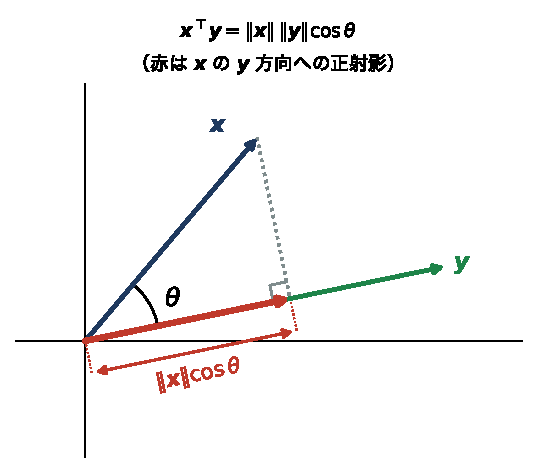
\includegraphics[width=0.62\linewidth]{figures/ch2_projection}
  \caption{内積の幾何学的意味。$\bm{x}$ を $\bm{y}$ の方向に射影した長さ $\|\bm{x}\|\cos\theta$ に、$\|\bm{y}\|$ を掛けたものが内積である。}
  \label{fig:projection}
\end{figure}

すなわち\textbf{内積とは、一方を他方の方向へ射影した長さに、その方向の長さを掛けたもの}である。
$\|\bm{y}\| = 1$ のときは内積そのものが射影の長さになる。
この見方は、第4回で「回帰とは射影である」という幾何学的理解につながる。


\subsection{内積と類似度}

\subsubsection{コサイン類似度}

内積 $\bm{x}^\top \bm{y} = \|\bm{x}\|\|\bm{y}\|\cos\theta$ は、
ベクトルの長さに依存してしまう。
例えば $\bm{x}$ を $2$ 倍すれば内積も $2$ 倍になるが、向きは変わっていない。
「向きの近さ」だけを測りたい場合は、長さで割って正規化する。

\begin{itembox}[l]{定義：コサイン類似度}
$\bm{x}, \bm{y} \neq \bm{0}$ に対して、
\begin{equation}
  \mathrm{cossim}(\bm{x}, \bm{y}) = \frac{\bm{x}^\top \bm{y}}{\|\bm{x}\| \, \|\bm{y}\|} = \cos\theta
  \;\in\; [-1, 1]
\end{equation}
を\textbf{コサイン類似度}（cosine similarity）と呼ぶ。
$1$ に近いほど2つのベクトルは同じ向き（似ている）、
$0$ なら無関係（直交）、$-1$ に近いほど逆向きであることを意味する。
\end{itembox}


\begin{figure}[H]
  \centering
  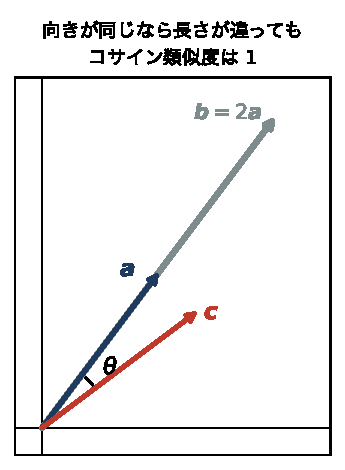
\includegraphics[width=0.5\linewidth]{figures/ch2_cossim}
  \caption{長さと向きの違い。$\bm{b} = 2\bm{a}$ は $\bm{a}$ より長いが向きは同じなので $\mathrm{cossim}(\bm{a},\bm{b}) = 1$ である。}
  \label{fig:cossim}
\end{figure}

コサイン類似度は、$\bm{x}$ と $\bm{y}$ をそれぞれ正規化してから内積をとったものに等しい：
\begin{equation}
  \mathrm{cossim}(\bm{x}, \bm{y}) = \left( \frac{\bm{x}}{\|\bm{x}\|} \right)^\top
  \left( \frac{\bm{y}}{\|\bm{y}\|} \right)
\end{equation}
したがって、あらかじめ正規化されたベクトル同士であれば、
内積そのものがコサイン類似度となる。

\subsubsection{例：文書の類似度}

3つの文書があり、単語「学習」「行列」「料理」の出現回数を数えて
3次元ベクトルで表したとする：
\begin{equation*}
  \bm{a} = (10, 8, 0)^\top, \qquad
  \bm{b} = (5, 4, 0)^\top, \qquad
  \bm{c} = (0, 1, 9)^\top
\end{equation*}
文書 $\bm{a}$ と $\bm{b}$ はどちらも機械学習の文書、$\bm{c}$ は料理の文書だとする。

ノルムは $\|\bm{a}\| = \sqrt{164} \approx 12.81$、$\|\bm{b}\| = \sqrt{41} \approx 6.40$、
$\|\bm{c}\| = \sqrt{82} \approx 9.06$ である。内積とコサイン類似度を計算すると
\begin{align*}
  \bm{a}^\top \bm{b} &= 50 + 32 + 0 = 82,
    &\mathrm{cossim}(\bm{a}, \bm{b}) &= \frac{82}{12.81 \times 6.40} \approx 1.00 \\
  \bm{a}^\top \bm{c} &= 0 + 8 + 0 = 8,
    &\mathrm{cossim}(\bm{a}, \bm{c}) &= \frac{8}{12.81 \times 9.06} \approx 0.07
\end{align*}
となる。$\bm{a}$ と $\bm{b}$ は長さが約2倍違うにもかかわらず、
向きがほぼ同じなのでコサイン類似度は $1$ に近い。
一方 $\bm{a}$ と $\bm{c}$ はほぼ直交しており、無関係であることが読み取れる。

このように、\textbf{内積は「関連の強さ」を1つの数値に要約する}。
次節で見る Attention 機構は、この性質を直接利用している。


\subsection{発展：内積と Attention}

本節では、現代AIの中核である \textbf{Transformer}\footnote{%
A. Vaswani et al., ``Attention Is All You Need,'' NeurIPS 2017.}
の \textbf{Attention}（注意機構）が、
本章で学んだ内積によって構成されていることを見る。
Attention の全体像は第13回で改めて扱うため、
本節では「内積が何をしているか」に焦点を当てる。
本節の内容は、この時点ですべてを理解することを求めるものではない。
まずは\textbf{なぜ内積を学ぶのか}を実感し、
第13回で再びこの節に戻ってきてほしい。

\subsubsection{単語をベクトルで表す}

自然言語処理では、各単語を $d$ 次元のベクトルで表現する。
これを\textbf{分散表現}（distributed representation）あるいは
\textbf{埋め込み}（embedding）と呼ぶ。
ここでは、その作り方を具体的に定める。

まず、扱う単語の全体を\textbf{語彙}（vocabulary）と呼び、
$\mathcal{V} = \{ w_1, w_2, \ldots, w_V \}$ とする（$V$ は語彙数、通常数万程度）。
$i$ 番目の単語 $w_i$ を、第 $i$ 成分だけが $1$ で他が $0$ である
$V$ 次元ベクトルで表す：
\begin{equation}
  \bm{o}_i = (0, \ldots, 0, \underset{\substack{\uparrow \\ \text{第 $i$ 成分}}}{1}, 0, \ldots, 0)^\top \in \mathbb{R}^{V}
\end{equation}
これを\textbf{ワンホットベクトル}（one-hot vector）と呼ぶ。
この表現では、異なる単語のベクトルは互いに直交し
（$i \neq j$ のとき $\bm{o}_i^\top \bm{o}_j = 0$）、
どの2語も同じだけ「無関係」になってしまう。
つまり\textbf{ワンホット表現では意味の近さを内積で測れない}。

そこで、各単語に $d$ 次元（$d \ll V$、例えば $d = 512$）の実ベクトルを割り当てる。

\begin{itembox}[l]{定義：埋め込み}
\textbf{埋め込み行列} $\bm{E} \in \mathbb{R}^{V \times d}$ の第 $i$ 行を
単語 $w_i$ の\textbf{埋め込みベクトル} $\bm{x}_i \in \mathbb{R}^d$ と定める：
\begin{equation}
  \bm{x}_i = \bm{E}^\top \bm{o}_i
\end{equation}
$\bm{E}$ の成分は、あらかじめ決めるのではなく\textbf{学習によって決定される}パラメータである。
\end{itembox}

この式が「第 $i$ 行を取り出す」操作になっていることは、成分で確かめられる。
$\bm{E}$ の $(k, j)$ 成分を $E_{kj}$ と書くと、
$\bm{E}^\top$ の第 $j$ 行は $(E_{1j}, E_{2j}, \ldots, E_{Vj})$ であるから、
これと $\bm{o}_i$ の内積は
\begin{equation}
  (\bm{x}_i)_j = \sum_{k=1}^{V} E_{kj} (\bm{o}_i)_k = E_{ij}
\end{equation}
となる（$\bm{o}_i$ は第 $i$ 成分のみ $1$ なので、和のうち $k = i$ の項だけが残る）。
すなわち $\bm{x}_i = (E_{i1}, \ldots, E_{id})^\top$ であり、確かに $\bm{E}$ の第 $i$ 行である。
このような操作を\textbf{埋め込みの参照}（embedding lookup）と呼ぶ。


\begin{figure}[H]
  \centering
  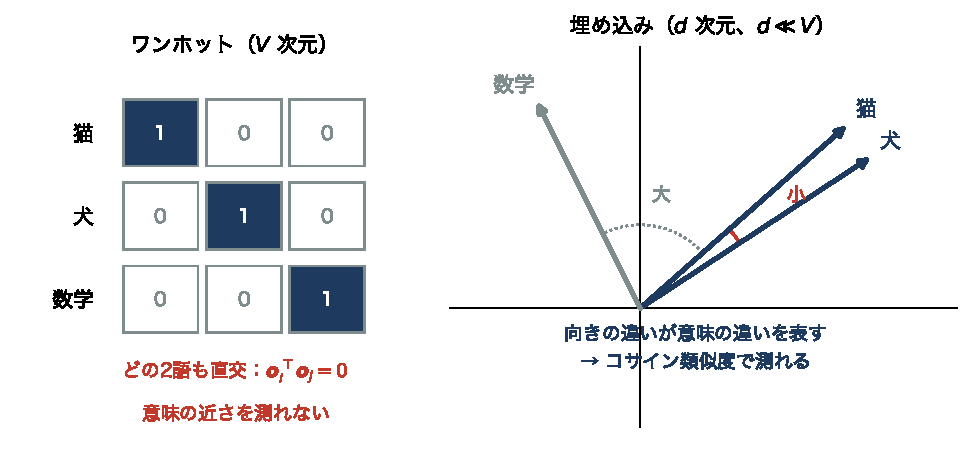
\includegraphics[width=0.95\linewidth]{figures/ch2_embedding}
  \caption{ワンホット表現と埋め込み。ワンホットではどの2語も直交するため意味の近さを測れないが、埋め込みでは向きの違いが意味の違いを表す。}
  \label{fig:embedding}
\end{figure}

学習は「文脈が似ている単語は似たベクトルになる」ように行われる。
その結果、前節のコサイン類似度で意味的な近さが測れるようになる。
例えば学習後には
\begin{equation*}
  \mathrm{cossim}(\bm{x}_{\text{猫}}, \bm{x}_{\text{犬}}) \gg
  \mathrm{cossim}(\bm{x}_{\text{猫}}, \bm{x}_{\text{数学}})
\end{equation*}
となることが期待される。
$V$ 次元で互いに直交していたワンホット表現が、
$d$ 次元の「意味の空間」に埋め込まれ、
向きの違いとして意味の違いが表現されるようになる、というのが埋め込みの要点である。

なお、記号 $\gg$ は「はるかに大きい」と読む。

\subsubsection{Query, Key, Value}

「その猫は魚を食べた」という文において、
「食べた」という語を理解するには「猫」（誰が）と「魚」（何を）に注目する必要がある。
この「どの語に注目すべきか」を内積で決めるのが Attention である。

ここで、単語ベクトル $\bm{x}$ をそのまま使って内積を計算するのではなく、
役割の異なる3つのベクトルに変換してから用いる。

\begin{itembox}[l]{定義：Query, Key, Value}
学習されるパラメータ行列
$\bm{W}_Q, \bm{W}_K \in \mathbb{R}^{d \times d_k}$、
$\bm{W}_V \in \mathbb{R}^{d \times d_v}$ を用いて、
単語ベクトル $\bm{x} \in \mathbb{R}^d$ から次の3つを作る：
\begin{align}
  \bm{q} &= \bm{W}_Q^\top \bm{x} \in \mathbb{R}^{d_k} &&\textbf{Query}（クエリ） \\
  \bm{k} &= \bm{W}_K^\top \bm{x} \in \mathbb{R}^{d_k} &&\textbf{Key}（キー） \\
  \bm{v} &= \bm{W}_V^\top \bm{x} \in \mathbb{R}^{d_v} &&\textbf{Value}（バリュー）
\end{align}
\end{itembox}

この変換もまた内積の集まりである。
例えば $\bm{W}_Q$ の第 $j$ 列を $\bm{u}_j \in \mathbb{R}^d$ とすると、
\begin{equation}
  q_j = \bm{u}_j^\top \bm{x} \qquad (j = 1, \ldots, d_k)
\end{equation}
であり、Query の各成分は単語ベクトルと学習された重みベクトルの内積である。
これは前節のニューロンの線形部分と同じ構造であり、
$d_k$ 個の内積を並べたもの、すなわち第3回で学ぶ行列とベクトルの積にほかならない。

3つのベクトルが表す役割は次のとおりである。
\begin{itemize}
  \item \textbf{Query} $\bm{q}$：「私は何を探しているか」という問い合わせ
  \item \textbf{Key} $\bm{k}$：「私は何を提供できるか」という見出し
  \item \textbf{Value} $\bm{v}$：「実際に渡す情報」という中身
\end{itemize}
図書館に例えれば、Query は検索語、Key は各本の背表紙、Value は本の中身である。
検索語と背表紙を照合して、合致した本の中身を取り出す、という仕組みである。

\paragraph{なぜ3つに分けるのか}
同じ単語でも、\textbf{探す側}に回るときと\textbf{探される側}に回るときでは、
必要な情報が異なる。
「食べた」という語は、動作の主体を探すときには「主語を探している」という Query として働き、
別の語から参照されるときには「動詞である」という Key として働く。
$\bm{W}_Q$ と $\bm{W}_K$ を別々に学習することで、
この非対称な役割を表現できる。

実際、もし $\bm{q}$ と $\bm{k}$ を同じベクトル（$\bm{x}$ そのもの）にしてしまうと、
スコアが $\bm{x}_i^\top \bm{x}_j = \bm{x}_j^\top \bm{x}_i$ と対称になり、
「$i$ が $j$ に注目する度合い」と「$j$ が $i$ に注目する度合い」が
常に等しくなってしまう。
内積は対称性をもつが、$\bm{W}_Q \neq \bm{W}_K$ とすることで
\begin{equation}
  \bm{q}_i^\top \bm{k}_j = (\bm{W}_Q^\top \bm{x}_i)^\top (\bm{W}_K^\top \bm{x}_j)
  \neq \bm{q}_j^\top \bm{k}_i \quad \text{（一般に）}
\end{equation}
となり、非対称な注目関係を表せるようになる。

また Value を分けるのは、\textbf{照合に使う情報}と\textbf{受け渡す情報}を
独立に設計できるようにするためである。
そのため $\bm{v}$ の次元 $d_v$ は $d_k$ と異なってよい。

\paragraph{自己注意と次元}
入力文の $n$ 個の単語すべてから Query, Key, Value を作り、
同じ文の中で照合を行う場合を\textbf{自己注意}（self-attention）と呼ぶ。
Transformer の基本構成要素はこれである。
代表的な設定では $d = 512$、$d_k = d_v = 64$ である。

\subsubsection{注目度を内積で測る}

Query $\bm{q}$ と各 Key $\bm{k}_i$ の\textbf{関連の強さ}を、内積で測る：
\begin{equation}
  \mathrm{score}(\bm{q}, \bm{k}_i) = \bm{q}^\top \bm{k}_i
  = \|\bm{q}\| \, \|\bm{k}_i\| \cos\theta_i
\end{equation}
前節で見たとおり、この値は $\bm{q}$ と $\bm{k}_i$ の向きが一致するほど大きくなる。
すなわち\textbf{「探しているもの」と「提供できるもの」が合致する単語のスコアが高くなる}。

\subsubsection{スコアを重みに変換する}

スコアは正にも負にもなり、合計も $1$ にならないため、そのままでは「重み」として使えない。
そこで\textbf{ソフトマックス関数}（softmax）で正規化する：
\begin{equation}
  \alpha_i = \frac{\exp(\mathrm{score}_i)}{\sum_{j=1}^{n} \exp(\mathrm{score}_j)}
\end{equation}
指数関数 $\exp$ は常に正であり、分母で全体の和を割っているので、
\begin{equation}
  \alpha_i > 0, \qquad \sum_{i=1}^{n} \alpha_i = 1
\end{equation}
が成り立つ。すなわち $\alpha_i$ は「単語 $i$ にどれだけ注目するか」の割合を表す。


\begin{figure}[H]
  \centering
  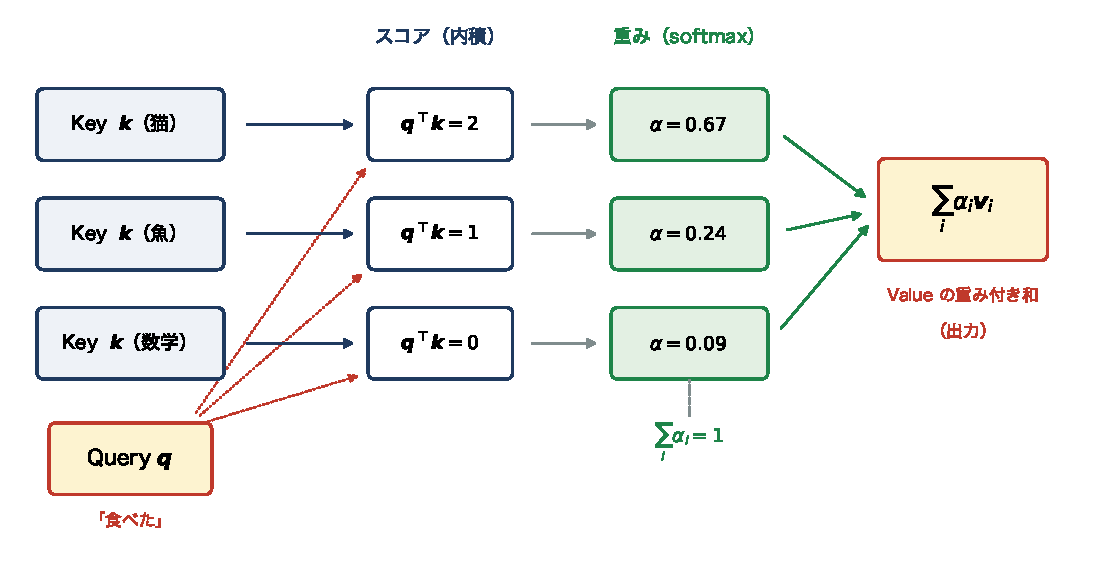
\includegraphics[width=0.95\linewidth]{figures/ch2_attention_flow}
  \caption{Attention のデータフロー。Query と各 Key の内積でスコアを計算し、ソフトマックスで重みに変換して、Value を混ぜ合わせる。}
  \label{fig:attnflow}
\end{figure}

最終的な出力は、Value の重み付き和である：
\begin{equation}
  \mathrm{Attention}(\bm{q}, K, V) = \sum_{i=1}^{n} \alpha_i \bm{v}_i
\end{equation}
注目度が高い単語の情報ほど、強く混ぜ合わされることになる。

\subsubsection{数値例}

「食べた」という Query に対し、「猫」「魚」「数学」の3つの Key があるとする。
簡単のため $d_k = 2$ とし、
\begin{equation*}
  \bm{q} = (1, 1)^\top, \qquad
  \bm{k}_1 = (1, 1)^\top, \quad
  \bm{k}_2 = (1, 0)^\top, \quad
  \bm{k}_3 = (-1, 1)^\top
\end{equation*}
とする（$\bm{k}_1$：猫、$\bm{k}_2$：魚、$\bm{k}_3$：数学）。
内積を計算すると
\begin{equation*}
  \bm{q}^\top \bm{k}_1 = 1 + 1 = 2, \qquad
  \bm{q}^\top \bm{k}_2 = 1 + 0 = 1, \qquad
  \bm{q}^\top \bm{k}_3 = -1 + 1 = 0
\end{equation*}
となる。ソフトマックスを適用すると、$\exp(2) \approx 7.39$、$\exp(1) \approx 2.72$、
$\exp(0) = 1$ より、分母は $7.39 + 2.72 + 1 = 11.11$ で
\begin{equation*}
  \alpha_1 \approx 0.67, \qquad \alpha_2 \approx 0.24, \qquad \alpha_3 \approx 0.09
\end{equation*}

\begin{figure}[H]
  \centering
  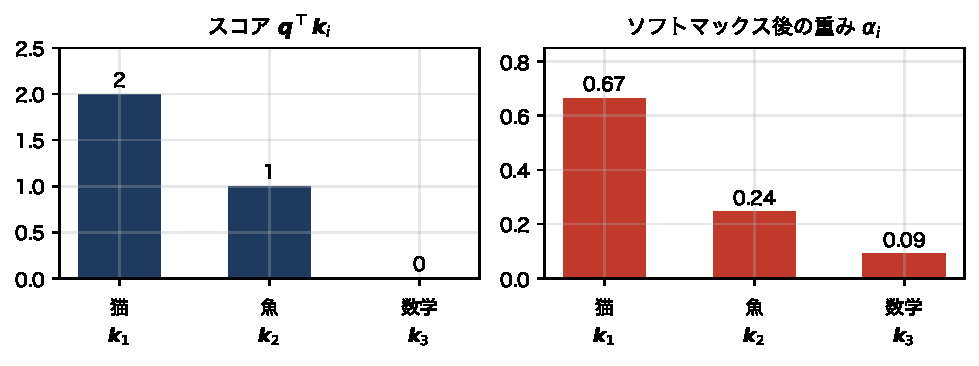
\includegraphics[width=0.92\linewidth]{figures/ch2_attention}
  \caption{内積で計算したスコアと、ソフトマックスによる重み。スコアの差が指数関数で強調され、合計が $1$ になる。}
  \label{fig:attention}
\end{figure}

を得る。「猫」に約67\%、「魚」に約24\%、「数学」に約9\%の注目が向けられる。
出力は $0.67\bm{v}_1 + 0.24\bm{v}_2 + 0.09\bm{v}_3$ となり、
「猫」の情報を中心に混ぜ合わせた表現が得られる。

\subsubsection{行列表記と $\sqrt{d_k}$}

実際には、多数の Query を同時に処理する。
$n$ 個の Query を縦に並べた $Q$、$m$ 個の Key を並べた $K$、Value を並べた $V$ を用いると、
すべての Query と Key の内積は一つの積 $QK^\top$ にまとまる。
この\textbf{行列}という概念は次回（第3回）で扱う。
結果として、Attention は次の一つの式で表される：
\begin{equation}
  \mathrm{Attention}(Q, K, V) = \mathrm{softmax}\!\left( \frac{QK^\top}{\sqrt{d_k}} \right) V
\end{equation}

ここで $\sqrt{d_k}$ で割る理由を、本章のノルムの言葉で説明する。
$\bm{q}$ と $\bm{k}$ の各成分が独立に平均 $0$、分散 $1$ 程度であるとすると、
内積 $\bm{q}^\top \bm{k} = \sum_{i=1}^{d_k} q_i k_i$ は $d_k$ 個の項の和であり、
その大きさはおよそ $\sqrt{d_k}$ に比例して増大する。
次元 $d_k$ が大きい（実際のモデルでは $64$ 程度）とスコアの絶対値が大きくなり、
ソフトマックスの指数関数によって最大値のみが $1$、他がほぼ $0$ という
極端な分布になってしまう。これを防ぐため、$\sqrt{d_k}$ で割ってスコアの尺度を揃えている。
これは\textbf{次元が上がるとノルムが大きくなる}という、本章で扱った性質に基づく調整である。

\subsubsection{まとめ}

Attention の本質は次の一文に要約される：
\begin{center}
  \textbf{「関連の強さを内積で測り、その重みで情報を混ぜ合わせる」}
\end{center}
本章で学んだ内積が、現代AIの中核をなす仕組みを直接支えている。
Transformer 全体の構造、multi-head attention、位置符号化などは第13回で扱う。


\subsection{発展：内積とニューラルネットワーク}

前節では、内積が Transformer の Attention を支えていることを見た。
本節では、もう一つの現代AIの柱である\textbf{ニューラルネットワーク}
（neural network）においても、内積が基本要素となっていることを見る。
前節と同様、全体像は第12回で改めて扱う。
本節では、本章で学んだ内積とノルムだけを用いて、
ニューロン1個が何を計算しているのかを正確に理解することを目標とする。

\subsubsection{ニューロン1個の計算}

ニューラルネットワークの最小単位を\textbf{ニューロン}（neuron）あるいは
ユニットと呼ぶ。1個のニューロンが行う計算は、次の2段階である。

\begin{itembox}[l]{定義：ニューロンの計算}
入力 $\bm{x} \in \mathbb{R}^d$、重み $\bm{w} \in \mathbb{R}^d$、バイアス $b \in \mathbb{R}$ に対して、
\begin{align}
  z &= \bm{w}^\top \bm{x} + b &&\text{（線形部分：内積とバイアス）} \\
  a &= \sigma(z) &&\text{（非線形部分：活性化関数）}
\end{align}
を計算する。$z$ を\textbf{重み付き和}（weighted sum）あるいは活性、$a$ を\textbf{出力}（output）と呼び、
$\sigma$ を\textbf{活性化関数}（activation function）と呼ぶ。
\end{itembox}


\begin{figure}[H]
  \centering
  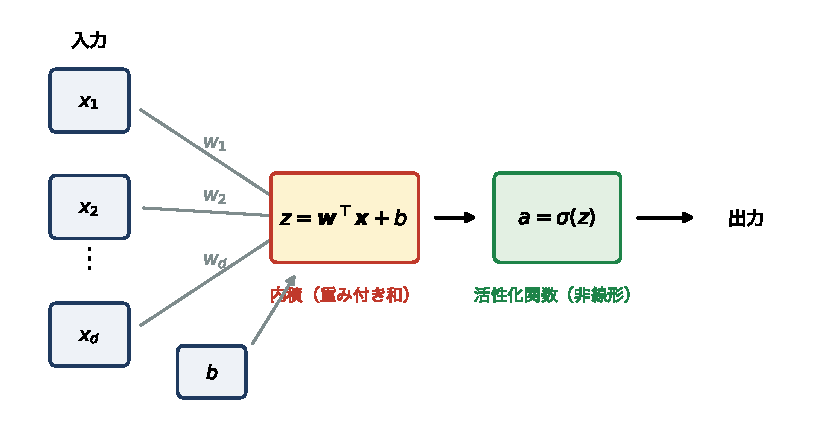
\includegraphics[width=0.88\linewidth]{figures/ch2_neuron_diagram}
  \caption{ニューロン1個の計算。入力と重みの内積にバイアスを加え（線形部分）、活性化関数を通す（非線形部分）。}
  \label{fig:neurondiag}
\end{figure}

第1段階の $\bm{w}^\top \bm{x} + b$ は、第1回で扱った線形モデルそのものである。
すなわち\textbf{ニューロンの線形部分は内積にほかならない}。
入力の各成分に重みを掛けて足し合わせる、という素朴な計算が、
ベクトルの言葉では1つの内積として簡潔に表される。

\subsubsection{ニューロンは何を検出しているのか}

なぜ内積を計算するのか。その意味は、本章で導いた幾何学的解釈から明らかになる：
\begin{equation}
  \bm{w}^\top \bm{x} = \|\bm{w}\| \, \|\bm{x}\| \cos\theta
\end{equation}
すなわち $z$ は、入力 $\bm{x}$ が重み $\bm{w}$ の向きとどれだけ一致しているかを測っている。

\begin{itemize}
  \item $\bm{x}$ が $\bm{w}$ と同じ向き（$\theta$ が小さい）$\Rightarrow$ $z$ が大きい $\Rightarrow$ 強く発火する
  \item $\bm{x}$ が $\bm{w}$ と直交（$\theta = \pi/2$）$\Rightarrow$ $z = 0$ $\Rightarrow$ 反応しない
  \item $\bm{x}$ が $\bm{w}$ と逆向き $\Rightarrow$ $z$ が負 $\Rightarrow$ 抑制される
\end{itemize}

つまり\textbf{重みベクトル $\bm{w}$ は、そのニューロンが検出したい「特徴の向き」を表している}。
学習とは、検出すべき向きを見つけることにほかならない。
前節の Attention が「Query と Key の一致度」を内積で測っていたのと、同じ構造である。

\subsubsection{決定境界と法線ベクトル}

バイアス $b$ の役割も幾何学的に理解できる。$z = 0$ となる入力の集合
\begin{equation}
  \{\, \bm{x} \in \mathbb{R}^d \mid \bm{w}^\top \bm{x} + b = 0 \,\}
\end{equation}
は、$d = 2$ のとき直線、$d = 3$ のとき平面、一般には\textbf{超平面}（hyperplane）と呼ばれる。
これを境に出力の符号が変わるため、\textbf{決定境界}（decision boundary）と呼ばれる。

この超平面上の任意の2点 $\bm{x}_1, \bm{x}_2$ に対して
$\bm{w}^\top \bm{x}_1 + b = \bm{w}^\top \bm{x}_2 + b = 0$ であるから、差をとると
\begin{equation}
  \bm{w}^\top (\bm{x}_1 - \bm{x}_2) = 0
\end{equation}
すなわち $\bm{w}$ は超平面に沿う任意の方向と直交する。
したがって\textbf{$\bm{w}$ は決定境界の法線ベクトル}であり、
$b$ は境界を原点からどれだけずらすかを決める。
この見方は、第10回のサポートベクターマシンでマージンを考える際の出発点となる。

\subsubsection{なぜ非線形が必要か}

第2段階の活性化関数 $\sigma$ には、次のような非線形関数が用いられる。
\begin{align}
  \text{ReLU：} \quad & \sigma(z) = \max(0, z) \\
  \text{シグモイド：} \quad & \sigma(z) = \frac{1}{1 + e^{-z}} \;\in\; (0, 1)
\end{align}

なぜ非線形関数が必要なのか。仮に $\sigma$ を恒等写像 $\sigma(z) = z$（線形）としてみよう。
2段重ねたとき、
\begin{equation}
  a_2 = \bm{w}_2^\top (\bm{w}_1^\top \bm{x} + b_1) + b_2
      = (\bm{w}_2^\top \bm{w}_1^\top) \bm{x} + (\bm{w}_2^\top b_1 + b_2)
\end{equation}
となり、これは結局 $\bm{x}$ についての1次式、すなわち\textbf{1層の線形モデルと同じ}である。
何層重ねても表現力は増えない。
\textbf{非線形関数を挟むことで初めて、層を深くする意味が生まれる}。

これが第12回の「ニューラルネットワーク＝線形変換＋非線形」という理解の核心である。

\subsubsection{数値例：ANDを計算するニューロン}

2入力 $\bm{x} = (x_1, x_2)^\top$ が $0$ または $1$ をとるとき、
論理積（AND）を計算するニューロンを作ってみよう。
$\bm{w} = (1, 1)^\top$、$b = -1.5$、活性化関数をステップ関数
（$z > 0$ なら $1$、そうでなければ $0$）とする。

\begin{center}
\begin{tabular}{cc|c|c}
  $x_1$ & $x_2$ & $z = \bm{w}^\top \bm{x} + b$ & 出力 $a$ \\
  \hline
  0 & 0 & $0 - 1.5 = -1.5$ & 0 \\
  0 & 1 & $1 - 1.5 = -0.5$ & 0 \\
  1 & 0 & $1 - 1.5 = -0.5$ & 0 \\
  1 & 1 & $2 - 1.5 = 0.5$ & 1 \\
\end{tabular}
\end{center}

確かに AND が実現されている。
決定境界 $x_1 + x_2 = 1.5$ は、点 $(1,1)$ とそれ以外の3点を分離する直線である。
法線ベクトル $\bm{w} = (1,1)^\top$ は、この直線に垂直な方向を向いている。


\begin{figure}[H]
  \centering
  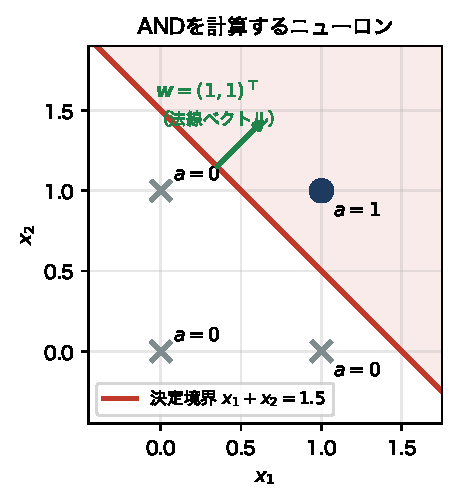
\includegraphics[width=0.52\linewidth]{figures/ch2_neuron}
  \caption{ANDを計算するニューロン。決定境界 $x_1 + x_2 = 1.5$ が点 $(1,1)$ とそれ以外を分離し、重み $\bm{w}$ は境界の法線ベクトルになっている。}
  \label{fig:neuron}
\end{figure}

なお、排他的論理和（XOR）は1個のニューロンでは実現できない。
1本の直線では $(0,1), (1,0)$ と $(0,0), (1,1)$ を分離できないからである。
これが\textbf{層を重ねる必要性}を示す古典的な例であり、第12回で改めて扱う。

\subsubsection{層：内積を並べたもの}

実際のニューラルネットワークでは、同じ入力に対して
多数のニューロンを並列に配置する。これを\textbf{層}（layer）と呼ぶ。
$m$ 個のニューロンがそれぞれ重み $\bm{w}_1, \ldots, \bm{w}_m \in \mathbb{R}^d$ を持つとき、
層の出力は
\begin{equation}
  \bm{a} =
  \begin{pmatrix} \sigma(\bm{w}_1^\top \bm{x} + b_1) \\ \sigma(\bm{w}_2^\top \bm{x} + b_2) \\ \vdots \\ \sigma(\bm{w}_m^\top \bm{x} + b_m) \end{pmatrix}
  \in \mathbb{R}^m
  \label{eq:layer-inner}
\end{equation}
となる。すなわち\textbf{層とは、$m$ 本の内積を並べたもの}である。
\begin{figure}[H]
  \centering
  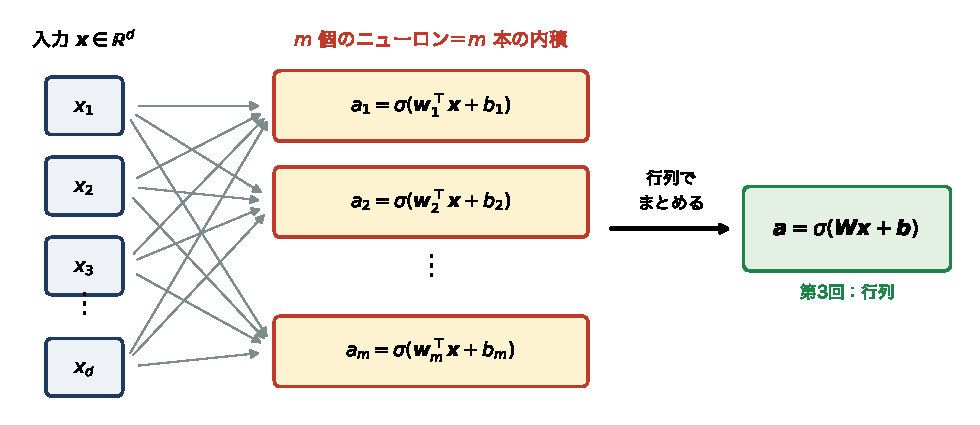
\includegraphics[width=0.95\linewidth]{figures/ch2_layer_diagram}
  \caption{層は $m$ 個のニューロンからなり、$m$ 本の内積を並べたものである。次回学ぶ行列を用いると、これは一つの式 $\bm{a} = \sigma(\bm{W}\bm{x}+\bm{b})$ にまとまる。}
  \label{fig:layerdiag}
\end{figure}

それぞれのニューロンが異なる向き $\bm{w}_i$ の特徴を検出し、
入力を $m$ 個の「特徴の強さ」に変換している。

式\eqref{eq:layer-inner}の $m$ 本の内積は、次回（第3回）で学ぶ\textbf{行列}を用いると
\begin{equation}
  \bm{a} = \sigma(\bm{W}\bm{x} + \bm{b}), \qquad \bm{W} \in \mathbb{R}^{m \times d}
\end{equation}
という一つの式にまとまる（$\sigma$ は各成分に適用する）。
$\bm{W}$ の第 $i$ 行が $\bm{w}_i^\top$ である。
この計算を層ごとに繰り返して出力へ至る流れを\textbf{順伝播}（forward propagation）と呼ぶ。

「複数の内積を一度に計算する」という操作が行列の積であり、
これは前節の Attention における $QK^\top$ とまったく同じ構造である。
次回、行列を導入することで、Attention とニューラルネットワークの両方が
同じ言葉で書けるようになる。

\subsubsection{まとめ}

ニューラルネットワークの1ニューロンは、次の一文に要約される：
\begin{center}
  \textbf{「入力と重みの内積で特徴の一致度を測り、非線形関数を通す」}
\end{center}
本章の内積が、Attention とニューラルネットワークという
現代AIの2つの柱を共通して支えている。
誤差逆伝播法による学習、深層化の効果などは第12回で扱う。


\subsection{まとめ}

本章の内容を整理する。

\begin{itemize}
  \item ベクトルはデータを並べたものであり、ノルム $\|\bm{x}\| = \sqrt{\bm{x}^\top \bm{x}}$ で長さを測る
  \item 内積 $\bm{x}^\top \bm{y} = \sum_i x_i y_i$ は対称性・線形性・正定値性をもつ
  \item コーシー・シュワルツの不等式から、内積は
    $\bm{x}^\top \bm{y} = \|\bm{x}\|\|\bm{y}\|\cos\theta$ と表され、長さと角度の情報を担う
  \item 内積が $0$ であることと直交は同値であり、第4回の最小二乗法の鍵となる
  \item 長さで正規化したコサイン類似度は、向きの近さを $[-1, 1]$ で測る
  \item Transformer の Attention は、Query と Key の内積で注目度を決めている
  \item ニューラルネットワークの1ニューロンは、内積で特徴の一致度を測り非線形関数を通す。
    重み $\bm{w}$ は検出したい特徴の向きであり、決定境界の法線ベクトルでもある
\end{itemize}

次回（第3回）は、複数のベクトルをまとめて扱う\textbf{行列}を導入し、
線形変換という視点から機械学習のモデルを捉え直す。
本章で見た $QK^\top$ や層の計算 $\bm{W}\bm{x}$ は、いずれも「複数の内積をまとめる」操作であり、
行列の積として統一的に表される。

特に、$N$ 件のデータ $\bm{x}_1, \ldots, \bm{x}_N$ を縦に積み上げると一つの行列となり、
モデルの予測全体が「行列とベクトルの積」として表される。
このとき予測は行列の列ベクトルの線形結合になっており、
第1回で導入した抽象的な仮説空間 $\mathcal{H}$ が、
具体的な幾何学的対象（列空間）として姿を現す。


\subsection{演習問題}

\begin{enumerate}
  \item \textbf{ノルムと内積の計算}\quad
    $\bm{x} = (2, -1, 2)^\top$、$\bm{y} = (1, 2, 2)^\top \in \mathbb{R}^3$ とする。
    \begin{enumerate}
      \item $\|\bm{x}\|$ と $\|\bm{y}\|$ を求めよ。
      \item $\bm{x}^\top \bm{y}$ を求めよ。
      \item $\bm{x}$ と $\bm{y}$ のコサイン類似度を求めよ。
      \item $\bm{x}$ を正規化した単位ベクトル $\bm{u}$ を求め、$\|\bm{u}\| = 1$ を確認せよ。
    \end{enumerate}

  \item \textbf{直交性}\quad
    $\bm{a} = (1, 2)^\top$ とする。
    \begin{enumerate}
      \item $\bm{a}$ と直交するベクトルを1つ求めよ。
      \item $\bm{a}$ と直交するベクトル全体の集合を、集合の記法を用いて表せ。
      \item $\bm{x} = (3, 1)^\top$ と $\bm{a}$ のなす角 $\theta$ について、
        $\cos\theta$ を求めよ。$\theta$ は鋭角か鈍角か。
    \end{enumerate}

  \item \textbf{内積の性質の証明}\quad
    任意の $\bm{x}, \bm{y} \in \mathbb{R}^d$ に対して、次の等式を内積の性質を用いて証明せよ。
    \begin{equation*}
      \|\bm{x} + \bm{y}\|^2 = \|\bm{x}\|^2 + 2\,\bm{x}^\top \bm{y} + \|\bm{y}\|^2
    \end{equation*}
    また、この結果を用いて、$\bm{x} \perp \bm{y}$ のとき
    $\|\bm{x} + \bm{y}\|^2 = \|\bm{x}\|^2 + \|\bm{y}\|^2$（三平方の定理）が成り立つことを示せ。

  \item \textbf{三角不等式}\quad
    問3の結果とコーシー・シュワルツの不等式を用いて、
    三角不等式 $\|\bm{x} + \bm{y}\| \leq \|\bm{x}\| + \|\bm{y}\|$ を証明せよ。

  \item \textbf{コサイン類似度と長さ}\quad
    $\bm{a} = (3, 4)^\top$、$\bm{b} = (6, 8)^\top$、$\bm{c} = (4, 3)^\top$ とする。
    \begin{enumerate}
      \item 内積 $\bm{a}^\top \bm{b}$ と $\bm{a}^\top \bm{c}$ をそれぞれ求めよ。
      \item コサイン類似度 $\mathrm{cossim}(\bm{a}, \bm{b})$ と
        $\mathrm{cossim}(\bm{a}, \bm{c})$ をそれぞれ求めよ。
      \item 内積で比較した場合とコサイン類似度で比較した場合で、
        $\bm{a}$ により「似ている」のはどちらのベクトルか。
        結果が異なる理由を、長さと向きの観点から説明せよ。
    \end{enumerate}

  \item \textbf{線形モデルと内積}\quad
    第1回の例2の線形モデル $h(\bm{x}) = 0.5 x_1 - 0.3 x_2 + 3$ を考える。
    \begin{enumerate}
      \item バイアス項を吸収した記法 $h(\bm{x}) = \bm{w}^\top \tilde{\bm{x}}$ で表すとき、
        $\bm{w}$ と $\tilde{\bm{x}}$ をそれぞれ書け。
      \item $\bm{x} = (25, 10)^\top$ に対する予測値を、内積の計算として求めよ。
      \item $h(\bm{x}) = 0$ を満たす $\bm{x}$ の集合は平面上でどのような図形になるか。
        また、$\bm{w}_{1:2} = (0.5, -0.3)^\top$ とその図形の関係を述べよ。
    \end{enumerate}

  \item \textbf{ニューロンと決定境界}\quad
    重み $\bm{w} = (2, -1)^\top$、バイアス $b = -1$ のニューロンを考える。
    活性化関数はステップ関数（$z > 0$ なら $1$、そうでなければ $0$）とする。
    \begin{enumerate}
      \item 入力 $\bm{x} = (2, 1)^\top$ に対する $z = \bm{w}^\top \bm{x} + b$ と出力を求めよ。
      \item 入力 $\bm{x} = (0, 3)^\top$ に対する $z$ と出力を求めよ。
      \item 決定境界 $\bm{w}^\top \bm{x} + b = 0$ を $x_2$ について解き、直線の式として書け。
      \item $\bm{w}$ がこの直線の法線ベクトルであることを、
        直線上の異なる2点を取って内積を計算することで確認せよ。
      \item 活性化関数を恒等写像 $\sigma(z) = z$ とし、このニューロンを2段重ねると
        1段の場合と同じ表現力しか持たないことを、式を書いて説明せよ。
    \end{enumerate}

  \item \textbf{Attention のスコア計算}\quad
    Query $\bm{q} = (2, 0)^\top$ と、3つの Key
    $\bm{k}_1 = (1, 0)^\top$、$\bm{k}_2 = (0, 2)^\top$、$\bm{k}_3 = (1, 1)^\top$ が与えられている。
    \begin{enumerate}
      \item 各スコア $\bm{q}^\top \bm{k}_i$（$i = 1, 2, 3$）を求めよ。
      \item ソフトマックスによる重み $\alpha_i$ を求めよ
        （$\exp(2) \approx 7.39$、$\exp(0) = 1$ を用いてよい）。
      \item 最も注目される Key はどれか。その理由を内積の幾何学的意味から説明せよ。
      \item $d_k$ が大きいとき、スコアを $\sqrt{d_k}$ で割る理由を説明せよ。
    \end{enumerate}
\end{enumerate}



\pagebreak

%===========================================
% Chapter 3
%===========================================
\section{行列と線形変換}

第2回では、1件のデータをベクトル $\bm{x} \in \mathbb{R}^d$ で表し、
線形モデルを内積 $\bm{w}^\top \bm{x}$ として理解した。
しかし実際の学習では、$N$ 件のデータをまとめて扱う必要がある。
本章では、数を長方形に並べた\textbf{行列}を導入し、
「行列とベクトルの積」という演算によって
モデル全体を一つの式で表せることを見る。

さらに本章の後半では、$N$ 件のデータを並べた\textbf{計画行列}を導入し、
モデルが表現できる予測の全体が\textbf{列空間}という部分空間になることを示す。
これにより、第1回で抽象的に定義した仮説空間 $\mathcal{H}$ が、
具体的な幾何学的対象として理解できるようになる。


\subsection{行列とは何か}

\subsubsection{行列の定義}

\begin{itembox}[l]{定義：行列}
実数を $m$ 行 $n$ 列の長方形に並べたものを
$m \times n$ \textbf{行列}（matrix）と呼び、本書では太字の大文字で表す：
\begin{equation}
  \bm{A} =
  \begin{pmatrix}
    a_{11} & a_{12} & \cdots & a_{1n} \\
    a_{21} & a_{22} & \cdots & a_{2n} \\
    \vdots & \vdots & \ddots & \vdots \\
    a_{m1} & a_{m2} & \cdots & a_{mn}
  \end{pmatrix}
  \in \mathbb{R}^{m \times n}
\end{equation}
$a_{ij}$ を第 $(i, j)$ \textbf{成分}と呼ぶ。
添字は「行が先、列が後」の順であり、$a_{ij}$ は第 $i$ 行・第 $j$ 列の成分を表す。
\end{itembox}

記号 $\mathbb{R}^{m \times n}$ は「$m$ 行 $n$ 列の実行列全体の集合」を表す。
$n = 1$ のとき $\mathbb{R}^{m \times 1}$ は列ベクトル全体、すなわち $\mathbb{R}^m$ と同一視される。
つまり\textbf{ベクトルは行列の特別な場合}である。

行列 $\bm{A} \in \mathbb{R}^{m \times n}$ は、2通りの見方ができる。
いずれも、行列をベクトルの集まりとみなす見方である。

\begin{itembox}[l]{定義：行と列の取り出し}
$\bm{A} \in \mathbb{R}^{m \times n}$ の第 $i$ 行の成分を並べたベクトル、
および第 $j$ 列の成分を並べたベクトルを、それぞれ
\begin{align}
  \bm{r}_i &= (a_{i1},\; a_{i2},\; \ldots,\; a_{in})^\top \;\in\; \mathbb{R}^{n}
    &&(i = 1, \ldots, m) \label{eq:row-vector} \\
  \bm{c}_j &= (a_{1j},\; a_{2j},\; \ldots,\; a_{mj})^\top \;\in\; \mathbb{R}^{m}
    &&(j = 1, \ldots, n)
\end{align}
と定める。どちらも\textbf{列ベクトル}である。
$\bm{A}$ の第 $i$ 行そのものは、$\bm{r}_i$ を横に倒した $\bm{r}_i^\top$（$1 \times n$ 行列）である。
これを用いると $\bm{A}$ は次の2通りに書ける：
\begin{equation}
  \bm{A} =
  \begin{pmatrix} \bm{r}_1^\top \\ \bm{r}_2^\top \\ \vdots \\ \bm{r}_m^\top \end{pmatrix}
  \qquad \text{（行による分解）}, \qquad
  \bm{A} = (\bm{c}_1\ \ \bm{c}_2\ \ \cdots\ \ \bm{c}_n)
  \qquad \text{（列による分解）}
\end{equation}
\end{itembox}

\subsubsubsection{なぜ $\bm{r}_i$ に転置が付くのか}

式\eqref{eq:row-vector}で $\bm{r}_i$ に $\top$ が付いていることに戸惑うかもしれない。
これは第2.1.1項の約束によるものである。
本書ではベクトルをすべて\textbf{列ベクトル}として扱い、
紙面では横に並べて書いて $\top$ を付けることで
「これは縦に並んだ列ベクトルである」と示す、という約束であった。
したがって式\eqref{eq:row-vector}は
\begin{equation}
  \bm{r}_i = \begin{pmatrix} a_{i1} \\ a_{i2} \\ \vdots \\ a_{in} \end{pmatrix} \in \mathbb{R}^n
\end{equation}
と書いているのと同じ意味であり、$\bm{r}_i$ は\textbf{列ベクトル}である。

一方、$\bm{A}$ の第 $i$ 行は横に並んだ $1 \times n$ 行列であるから、
$\bm{r}_i$ ではなく\textbf{その転置 $\bm{r}_i^\top$} が第 $i$ 行に一致する。
つまり $\top$ は2つの役割で現れており、混同しないよう注意してほしい。
\begin{itemize}
  \item 式\eqref{eq:row-vector}の $\top$：横書きの組が\textbf{列}ベクトルであることを示す（表記上の約束）
  \item $\bm{r}_i^\top$ の $\top$：列ベクトル $\bm{r}_i$ を\textbf{横に倒す}操作（第 $i$ 行そのもの）
\end{itemize}

この約束のおかげで、第 $i$ 行と $\bm{x} \in \mathbb{R}^n$ の内積が
$\bm{r}_i^\top \bm{x}$ と自然に書ける。
$\bm{r}_i, \bm{x}$ がともに列ベクトル（$n$ 次元）なので、
これは第2回の内積の記法 $\bm{x}^\top\bm{y}$ とまったく同じ形である。

\subsubsubsection{次元の確認}

次元を取り違えやすいので、しっかり確認してほしい。
\begin{itemize}
  \item 第 $i$ 行 $\bm{r}_i^\top$：成分は $n$ 個（$=$ 列の本数）。行は $m$ 本ある
  \item 第 $j$ 列 $\bm{c}_j$：成分は $m$ 個（$=$ 行の本数）。列は $n$ 本ある
\end{itemize}
すなわち、1本の行は横に $n$ 個の成分が並んだものだから $\bm{r}_i \in \mathbb{R}^n$ であり、
1本の列は縦に $m$ 個の成分が並んだものだから $\bm{c}_j \in \mathbb{R}^m$ である。
行の長さと列の長さで $m$ と $n$ が入れ替わる点に注意する。

本章では特に\textbf{列による分解}が重要になる。

\subsubsection{転置}

行と列を入れ替える操作を\textbf{転置}（transpose）と呼び、$\bm{A}^\top$ と書く：
\begin{equation}
  (\bm{A}^\top)_{ij} = a_{ji}, \qquad \bm{A} \in \mathbb{R}^{m \times n} \;\Rightarrow\; \bm{A}^\top \in \mathbb{R}^{n \times m}
\end{equation}
第2回で用いた $\bm{x}^\top$ は、$d \times 1$ 行列（列ベクトル）を
$1 \times d$ 行列（行ベクトル）に変える操作であった。

\subsubsection{行列の和とスカラー倍}

同じ大きさの行列同士の和、およびスカラー倍は、成分ごとに定める：
\begin{equation}
  (\bm{A} + \bm{B})_{ij} = a_{ij} + b_{ij}, \qquad (c\bm{A})_{ij} = c\, a_{ij}
\end{equation}


\subsection{行列とベクトルの積}

\subsubsection{定義と2つの見方}

\begin{itembox}[l]{定義：行列とベクトルの積}
$\bm{A} \in \mathbb{R}^{m \times n}$ と $\bm{x} \in \mathbb{R}^n$ に対して、
積 $\bm{A}\bm{x} \in \mathbb{R}^m$ を次で定める：
\begin{equation}
  (\bm{A}\bm{x})_i = \sum_{j=1}^{n} a_{ij} x_j \qquad (i = 1, \ldots, m)
\end{equation}
$\bm{A}$ の列数と $\bm{x}$ の次元が一致していなければ、積は定義されないことに注意する。
\end{itembox}

この積には、次の2つの見方がある。どちらも正しく、場面に応じて使い分ける。

\paragraph{見方1：行との内積}
$\bm{A}$ の第 $i$ 行を $\bm{r}_i^\top$ とすると、
\begin{equation}
  \bm{A}\bm{x} =
  \begin{pmatrix} \bm{r}_1^\top \bm{x} \\ \bm{r}_2^\top \bm{x} \\ \vdots \\ \bm{r}_m^\top \bm{x} \end{pmatrix}
\end{equation}
すなわち、積の第 $i$ 成分は第 $i$ 行と $\bm{x}$ の内積である。
$m$ 個の内積をまとめて計算しているとみなせる。

\paragraph{見方2：列の線形結合}
$\bm{A}$ の第 $j$ 列を $\bm{c}_j$ とすると、
\begin{equation}
  \bm{A}\bm{x} = x_1 \bm{c}_1 + x_2 \bm{c}_2 + \cdots + x_n \bm{c}_n = \sum_{j=1}^{n} x_j \bm{c}_j
  \label{eq:col-combination}
\end{equation}
すなわち、積は\textbf{$\bm{A}$ の列ベクトルを、$\bm{x}$ の成分を係数として足し合わせたもの}である。
このように、ベクトルにスカラーを掛けて足し合わせたものを\textbf{線形結合}（linear combination）と呼ぶ。

\noindent
\textbf{確認}\quad 式\eqref{eq:col-combination}の第 $i$ 成分を計算すると
\begin{equation}
  \left( \sum_{j=1}^{n} x_j \bm{c}_j \right)_i = \sum_{j=1}^{n} x_j (\bm{c}_j)_i = \sum_{j=1}^{n} x_j a_{ij}
\end{equation}
となり、定義と一致する（$\bm{c}_j$ の第 $i$ 成分は $a_{ij}$ である）。

\subsubsubsection{見方2の幾何学的な意味}

式\eqref{eq:col-combination}は、$\bm{A}\bm{x}$ が\textbf{つねに列ベクトル
$\bm{c}_1, \ldots, \bm{c}_n$ の線形結合として表される}ことを述べている。
言い換えれば、$\bm{x}$ をどのように選んでも、
$\bm{A}\bm{x}$ は列ベクトルたちが\textbf{張る}空間の中にしか現れない。

例えば $\bm{A} \in \mathbb{R}^{3 \times 2}$ で、2本の列 $\bm{c}_1, \bm{c}_2$ が
平行でない場合を考えよう
（この条件を一般化したものが、第3.2.3項で定義する\textbf{線形独立}である）。
$\bm{x} = (x_1, x_2)^\top$ を $\mathbb{R}^2$ 全体で動かしたとき、
$\bm{A}\bm{x} = x_1\bm{c}_1 + x_2\bm{c}_2$ が取りうる値の全体は、
$\mathbb{R}^3$ の中の\textbf{原点を通る平面}になる（図\ref{fig:span}）。
$\mathbb{R}^3$ 全体（3次元）ではなく、2次元の平面にとどまる点が重要である。

この「列ベクトルが張る空間」が第3.5節で定義する\textbf{列空間}であり、
線形モデルが表現できる予測の全体を表す。
第4回で学ぶ最小二乗法は、目標のベクトルがこの空間の外にあるとき、
その中で最も近い点を探す問題として定式化される。

なお、$\bm{c}_1$ と $\bm{c}_2$ が平行な場合は、
どのように線形結合しても同じ直線上にしか行けないため、
張られる空間は平面ではなく\textbf{直線}になる。
このように「張られる空間の次元」がモデルの自由度を決めており、
これを測る量が第3.5.4項の\textbf{ランク}である。

\subsubsection{例}

\begin{equation*}
  \bm{A} = \begin{pmatrix} 1 & 2 \\ 3 & 4 \\ 5 & 6 \end{pmatrix} \in \mathbb{R}^{3 \times 2},
  \qquad \bm{x} = \begin{pmatrix} 2 \\ -1 \end{pmatrix} \in \mathbb{R}^2
\end{equation*}
のとき、見方1（行との内積）では
\begin{equation*}
  \bm{A}\bm{x} = \begin{pmatrix} 1 \cdot 2 + 2 \cdot (-1) \\ 3 \cdot 2 + 4 \cdot (-1) \\ 5 \cdot 2 + 6 \cdot (-1) \end{pmatrix}
  = \begin{pmatrix} 0 \\ 2 \\ 4 \end{pmatrix}
\end{equation*}
見方2（列の線形結合）では
\begin{equation*}
  \bm{A}\bm{x} = 2 \begin{pmatrix} 1 \\ 3 \\ 5 \end{pmatrix} - 1 \begin{pmatrix} 2 \\ 4 \\ 6 \end{pmatrix}
  = \begin{pmatrix} 2 \\ 6 \\ 10 \end{pmatrix} - \begin{pmatrix} 2 \\ 4 \\ 6 \end{pmatrix}
  = \begin{pmatrix} 0 \\ 2 \\ 4 \end{pmatrix}
\end{equation*}
当然ながら結果は一致する。
この例を見方2で図示したものが図\ref{fig:span}である。
$\bm{A}\bm{x}$ は $\bm{c}_1$ を $2$ 倍したものから $\bm{c}_2$ を引いた点であり、
2本の列が張る平面の上に位置している。

\begin{figure}[H]
  \centering
  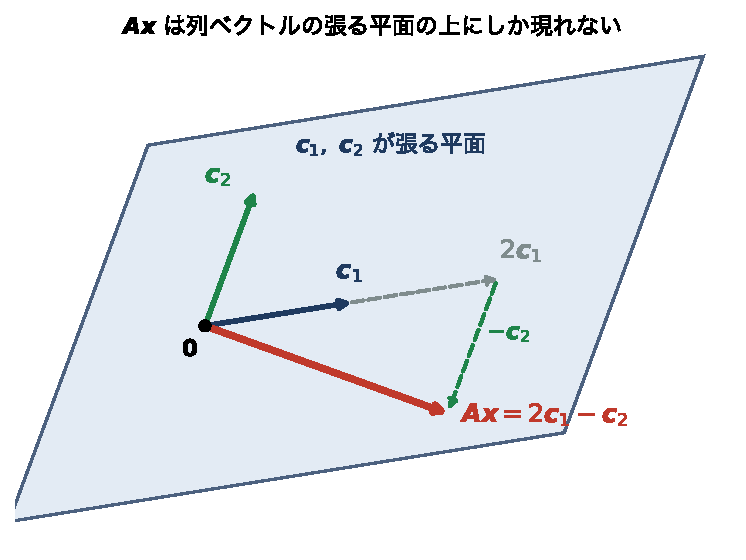
\includegraphics[width=0.74\linewidth]{figures/ch3_span}
  \caption{見方2（列の線形結合）の幾何学的な意味（模式図）。
    $\bm{A}\bm{x}$ は列ベクトル $\bm{c}_1, \bm{c}_2$ の線形結合であるから、
    $\bm{x}$ をどう選んでも、2本の列が張る平面の上にしか現れない。}
  \label{fig:span}
\end{figure}

\subsubsection{線形独立と張られる空間}

前項で「2本の列が平行でない場合」という条件を置いた。
この条件を一般の本数に拡張したものが\textbf{線形独立}である。

\begin{itembox}[l]{定義：線形独立・線形従属}
ベクトル $\bm{c}_1, \ldots, \bm{c}_n \in \mathbb{R}^m$ が\textbf{線形独立}
（linearly independent）であるとは、
\begin{equation}
  a_1 \bm{c}_1 + a_2 \bm{c}_2 + \cdots + a_n \bm{c}_n = \bm{0}
  \;\Longrightarrow\; a_1 = a_2 = \cdots = a_n = 0
  \label{eq:lin-indep}
\end{equation}
が成り立つことをいう。
すなわち、線形結合が零ベクトルになるのは、
係数がすべて $0$ という自明な場合に限る、ということである。
線形独立でないとき\textbf{線形従属}（linearly dependent）という。
\end{itembox}

\subsubsubsection{定義の読み方}

この定義は一見わかりにくいが、
\textbf{「どのベクトルも、他のベクトルの線形結合では表せない」}
と言い換えられる。理由を確かめよう。

線形従属、すなわち式\eqref{eq:lin-indep}が成り立たないとする。
このとき、すべてが $0$ ではない係数 $a_1, \ldots, a_n$ で
$a_1\bm{c}_1 + \cdots + a_n\bm{c}_n = \bm{0}$ となるものが存在する。
$0$ でない係数の一つを $a_k \neq 0$ とすると、$a_k \bm{c}_k$ を左辺に残して移項し、
両辺を $a_k$ で割れば
\begin{equation}
  \bm{c}_k = -\frac{1}{a_k} \sum_{j \neq k} a_j \bm{c}_j
\end{equation}
となる。つまり $\bm{c}_k$ が他のベクトルの線形結合で表せてしまう。
逆に、あるベクトルが他の線形結合で表せるなら、
移項すれば自明でない係数の組が作れるので線形従属である。
したがって両者は同値である。

\subsubsubsection{2本の場合：平行かどうか}

$n = 2$ のときは、幾何学的に単純な判定になる。
$\bm{c}_1, \bm{c}_2$ が線形従属であるとは、
$a_1\bm{c}_1 + a_2\bm{c}_2 = \bm{0}$ を満たす自明でない係数があることだから、
例えば $a_2 \neq 0$ として $\bm{c}_2 = -(a_1/a_2)\bm{c}_1$、
すなわち\textbf{一方が他方のスカラー倍}である。
これは2本の矢印が\textbf{同じ直線上にある（平行である）}ことを意味する。

\subsubsubsection{張られる空間の次元}

線形独立かどうかは、\textbf{張られる空間の大きさ}を決める（図\ref{fig:independence}）。
\begin{itemize}
  \item \textbf{線形独立}のとき：$\bm{c}_1, \bm{c}_2$ の線形結合は平面全体を覆う。
    張られる空間は\textbf{2次元}である
  \item \textbf{線形従属}のとき：どう線形結合しても同じ直線上にしか行けない。
    張られる空間は\textbf{1次元}にとどまる
\end{itemize}
本数を $n$ 本に増やしても同じである。
$n$ 本のうち線形独立なものが $r$ 本であれば、
張られる空間の次元は $n$ ではなく $r$ になる。

\begin{figure}[H]
  \centering
  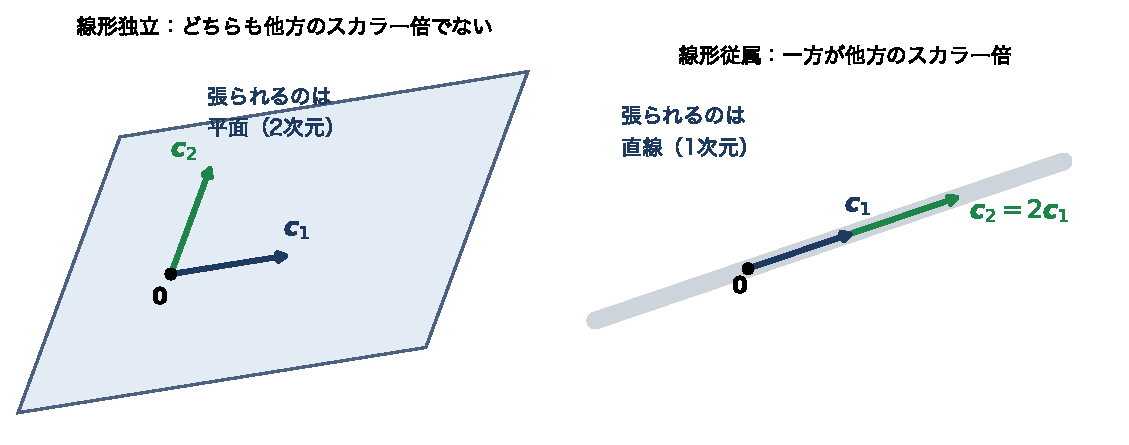
\includegraphics[width=0.95\linewidth]{figures/ch3_independence}
  \caption{線形独立と線形従属（模式図）。
    左：2本が平行でなければ、線形結合は平面（2次元）を張る。
    右：一方が他方のスカラー倍であれば、どう線形結合しても直線（1次元）から出られない。}
  \label{fig:independence}
\end{figure}

この「張られる空間の次元」こそが、
第3.5.4項で定義する\textbf{ランク}であり、
モデルが実際に表現できる自由度を表す量である。
線形従属な列があるということは、
その列が他の列で説明できてしまい\textbf{新しい情報を加えていない}ということであり、
第3.5.5項で扱う多重共線性の問題につながる。

\subsubsection{行列の積}

$\bm{A} \in \mathbb{R}^{m \times n}$、$\bm{B} \in \mathbb{R}^{n \times p}$ に対して、
積 $\bm{A}\bm{B} \in \mathbb{R}^{m \times p}$ を
\begin{equation}
  (\bm{A}\bm{B})_{ij} = \sum_{k=1}^{n} a_{ik} b_{kj}
\end{equation}
で定める。$\bm{A}$ の第 $i$ 行を $\bm{r}_i^\top$、$\bm{B}$ の第 $j$ 列を $\bm{c}_j$ と書けば、
これは\textbf{「$\bm{A}$ の第 $i$ 行と $\bm{B}$ の第 $j$ 列の内積」}にほかならない：
\begin{equation}
  (\bm{A}\bm{B})_{ij} = \bm{r}_i^\top \bm{c}_j
\end{equation}
$\bm{A}$ の列数と $\bm{B}$ の行数がともに $n$ で一致していなければ
内積が定義できないため、積も定義されない。

\begin{figure}[H]
  \centering
  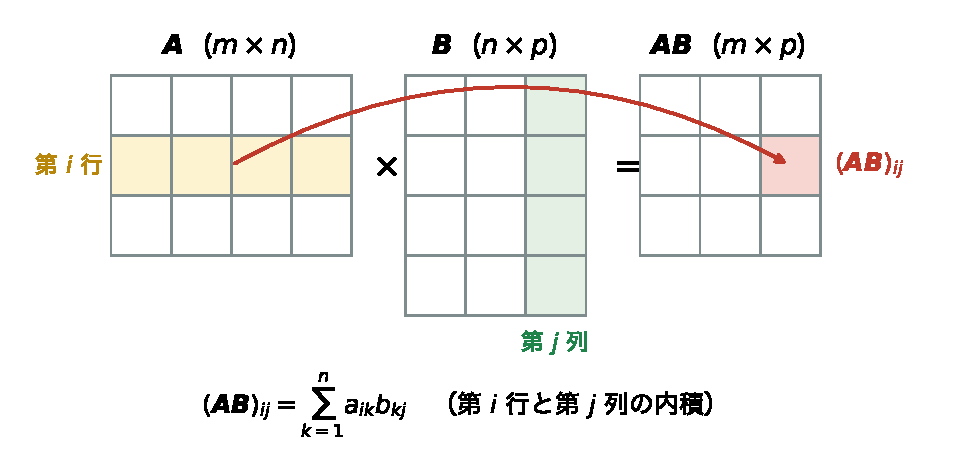
\includegraphics[width=0.88\linewidth]{figures/ch3_matmul}
  \caption{行列の積の意味。$\bm{A}\bm{B}$ の $(i, j)$ 成分は、
    $\bm{A}$ の第 $i$ 行と $\bm{B}$ の第 $j$ 列の内積である。
    $\bm{A}\bm{B}$ 全体は、$\bm{A}$ の $m$ 本の行と $\bm{B}$ の $p$ 本の列の、
    すべての組合せの内積を並べた表にあたる。}
  \label{fig:matmul}
\end{figure}

図\ref{fig:matmul}が示すとおり、$\bm{A}\bm{B}$ の1つの成分を得るには
1組の内積を計算すればよく、積の行列全体は
\textbf{$m \times p$ 通りすべての組合せの内積を並べた表}である。
すなわち行列の積とは、\textbf{多数の内積を一度にまとめて計算する操作}である。
第2回で「複数の内積をまとめる」と述べたのは、この演算のことであった。

なお、行列とベクトルの積 $\bm{A}\bm{x}$ は、$p = 1$ の特別な場合にあたる。
このとき $\bm{B}$ は1本の列 $\bm{x}$ だけからなり、
結果は $m$ 個の内積を縦に並べた $m$ 次元ベクトルになる。
これは第3.2.1.1項の見方1にほかならない。

なお、行列の積は一般に可換でない（$\bm{A}\bm{B} \neq \bm{B}\bm{A}$）ことに注意する。
一方、転置については次が成り立つ：
\begin{equation}
  (\bm{A}\bm{B})^\top = \bm{B}^\top \bm{A}^\top
\end{equation}
順序が入れ替わる点に注意する。


\subsection{線形写像}

\subsubsection{行列は写像である}

行列 $\bm{A} \in \mathbb{R}^{m \times n}$ を固定すると、
ベクトル $\bm{x} \in \mathbb{R}^n$ に対して $\bm{A}\bm{x} \in \mathbb{R}^m$ を対応させる関数
\begin{equation}
  f_{\bm{A}} : \mathbb{R}^n \to \mathbb{R}^m, \qquad f_{\bm{A}}(\bm{x}) = \bm{A}\bm{x}
\end{equation}
が定まる。第1回で学んだ関数の記法である。
すなわち\textbf{行列は $n$ 次元空間から $m$ 次元空間への写像}とみなせる。

\begin{itembox}[l]{定義：線形写像}
写像 $f : \mathbb{R}^n \to \mathbb{R}^m$ が、任意の $\bm{x}, \bm{y} \in \mathbb{R}^n$、
$c \in \mathbb{R}$ に対して
\begin{align}
  f(\bm{x} + \bm{y}) &= f(\bm{x}) + f(\bm{y}) \\
  f(c\bm{x}) &= c\, f(\bm{x})
\end{align}
を満たすとき、$f$ を\textbf{線形写像}（linear map）と呼ぶ。
\end{itembox}

行列による写像 $f_{\bm{A}}(\bm{x}) = \bm{A}\bm{x}$ は線形写像である。実際、
\begin{equation}
  \bm{A}(\bm{x} + \bm{y}) = \bm{A}\bm{x} + \bm{A}\bm{y}, \qquad \bm{A}(c\bm{x}) = c\,\bm{A}\bm{x}
\end{equation}
が成分計算から直ちに確かめられる。逆に、任意の線形写像は行列で表せることが知られている。
すなわち\textbf{線形写像と行列は同じものの2つの表現}である。

\subsubsubsection{線形写像が何をしているか}

線形写像を $n = m = 2$ の場合で図示したものが図\ref{fig:linearmap}である。
左が定義域、右がその像であり、$\bm{A}$ を掛けることで
空間全体が引き伸ばされ、傾けられている。

この図から、線形写像の性質が3つ読み取れる。
\begin{itemize}
  \item \textbf{等間隔の格子が、等間隔の格子に写る}。
    直線は直線に写り、平行な直線は平行なまま保たれる
  \item \textbf{原点は原点に写る}。実際 $\bm{A}\bm{0} = \bm{0}$ である
  \item \textbf{平行四辺形は平行四辺形に写る}。
    これは加法性 $\bm{A}(\bm{x}+\bm{y}) = \bm{A}\bm{x} + \bm{A}\bm{y}$ の図形的な表現である
\end{itemize}

3つ目について補足する。
左の図では、$\bm{x}$ と $\bm{y}$ を2辺とする平行四辺形の対角線が $\bm{x}+\bm{y}$ であった。
右の図でも、$\bm{A}\bm{x}$ と $\bm{A}\bm{y}$ を2辺とする平行四辺形の対角線が
$\bm{A}(\bm{x}+\bm{y})$ になっている。
すなわち「先に足してから写す」か「先に写してから足す」かで結果が変わらない。
これが加法性である。
同様に、斉次性 $\bm{A}(c\bm{x}) = c\,\bm{A}\bm{x}$ は
「矢印を $c$ 倍してから写す」ことと「写してから $c$ 倍する」ことが一致する、
という性質である。

\begin{figure}[H]
  \centering
  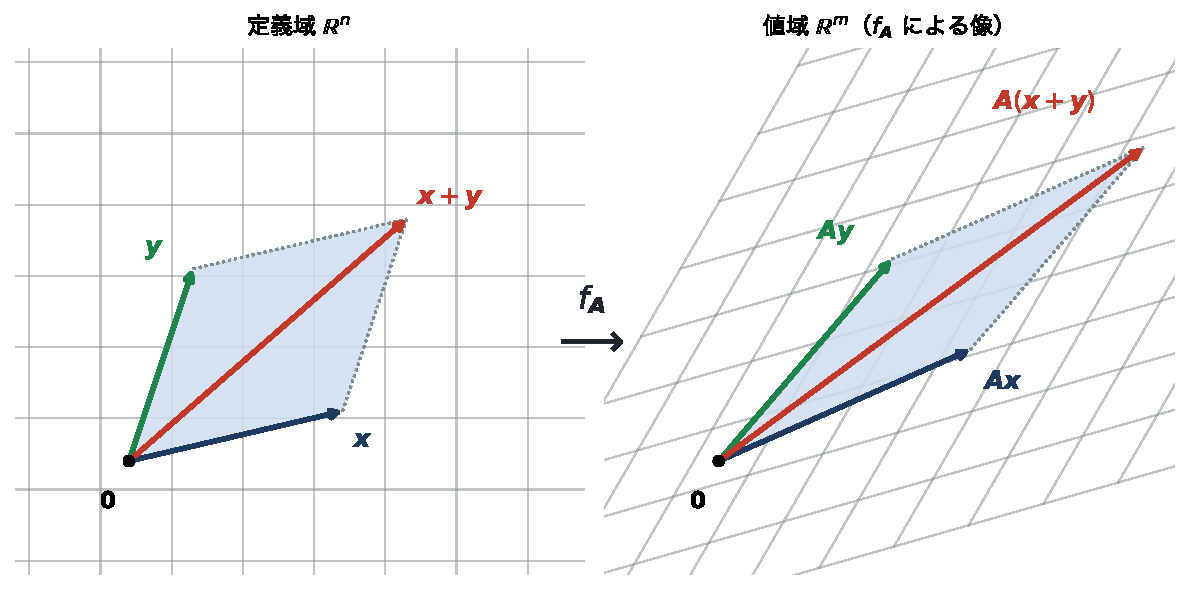
\includegraphics[width=0.95\linewidth]{figures/ch3_linearmap}
  \caption{線形写像 $f_{\bm{A}}(\bm{x}) = \bm{A}\bm{x}$ のはたらき（$n = m = 2$ の例）。
    格子は格子に、原点は原点に、平行四辺形は平行四辺形に写る。
    右図で $\bm{A}\bm{x}, \bm{A}\bm{y}$ の作る平行四辺形の対角線が
    $\bm{A}(\bm{x}+\bm{y})$ になっていることが、加法性にあたる。}
  \label{fig:linearmap}
\end{figure}

\subsubsection{線形性が意味すること}

線形写像は「直線を直線に、原点を原点に写す」写像である。
$f(\bm{0}) = f(0 \cdot \bm{0}) = 0 \cdot f(\bm{0}) = \bm{0}$ より、原点は必ず原点に移る。

ここで注意すべきは、第1回の線形モデル
\begin{equation}
  h(\bm{x}; \bm{w}) = w_0 + \bm{w}_{1:d}^\top \bm{x}
\end{equation}
は、$w_0 \neq 0$ のとき\textbf{線形写像ではない}。
実際、線形写像ならば $f(\bm{0}) = \bm{0}$ でなければならないが、
\begin{equation}
  h(\bm{0}; \bm{w}) = w_0 + \bm{w}_{1:d}^\top \bm{0} = w_0 \neq 0
\end{equation}
だからである。
（逆に $w_0 = 0$ のときは $h(\bm{x}) = \bm{w}_{1:d}^\top \bm{x}$ となり、これは線形写像である。）

このような写像は、線形写像に定数ベクトルを加えたものとして特徴づけられる。

\begin{itembox}[l]{定義：アフィン写像}
写像 $g : \mathbb{R}^n \to \mathbb{R}^m$ が、ある行列 $\bm{A} \in \mathbb{R}^{m \times n}$ と
ベクトル $\bm{b} \in \mathbb{R}^m$ を用いて
\begin{equation}
  g(\bm{x}) = \bm{A}\bm{x} + \bm{b}
\end{equation}
と書けるとき、$g$ を\textbf{アフィン写像}（affine map）と呼ぶ。
$\bm{b} = \bm{0}$ の場合が線形写像であり、
\textbf{線形写像はアフィン写像の特別な場合}である。
\end{itembox}

線形写像が「原点を原点に写す」のに対し、アフィン写像は
「線形写像で変換したうえで、全体を $\bm{b}$ だけ平行移動する」写像である。
直線を直線に写す性質は保たれるが、原点は一般に原点に移らない。

線形性の2条件は、アフィン写像では次のように崩れる。
$\bm{b} \neq \bm{0}$ のとき
\begin{align}
  g(\bm{x} + \bm{y}) &= \bm{A}(\bm{x} + \bm{y}) + \bm{b}
    = g(\bm{x}) + g(\bm{y}) - \bm{b} \;\neq\; g(\bm{x}) + g(\bm{y}) \\
  g(c\bm{x}) &= c\bm{A}\bm{x} + \bm{b}
    = c\, g(\bm{x}) + (1 - c)\bm{b} \;\neq\; c\, g(\bm{x}) \quad (c \neq 1)
\end{align}
いずれも余分な $\bm{b}$ の項が残る。

第2回で行った「バイアス項の吸収」、すなわち入力に定数 $1$ を付け加えて
$\tilde{\bm{x}} = (1, x_1, \ldots, x_d)^\top$ とする操作は、
アフィン写像を1次元高い空間の線形写像として扱うための技法である。
実際、$h(\bm{x}; \bm{w}) = \bm{w}^\top \tilde{\bm{x}}$ と書けば、
$\tilde{\bm{x}}$ を入力とみなす限りこれは線形（$\mathbb{R}^{d+1} \to \mathbb{R}$）である。
このように書き換えられるおかげで、以降の議論ではバイアス項を特別扱いせずに済む。


\subsection{計画行列}

\subsubsection{データをまとめる}

ここまでは1件のデータ $\bm{x}$ を扱ってきた。
$N$ 件の訓練データ $\bm{x}_1, \ldots, \bm{x}_N \in \mathbb{R}^d$ をまとめて扱うため、
各データを行として縦に積み上げた行列を考える。

\begin{itembox}[l]{定義：計画行列}
$N$ 件の訓練データ $\bm{x}_i = (x_{i1}, \ldots, x_{id})^\top$ に対して、
バイアス項のための定数列 $1$ を加えた行列
\begin{equation}
  \bm{X} =
  \begin{pmatrix}
    1 & x_{11} & x_{12} & \cdots & x_{1d} \\
    1 & x_{21} & x_{22} & \cdots & x_{2d} \\
    \vdots & \vdots & \vdots & & \vdots \\
    1 & x_{N1} & x_{N2} & \cdots & x_{Nd}
  \end{pmatrix}
  \in \mathbb{R}^{N \times (d+1)}
\end{equation}
を\textbf{計画行列}（design matrix）と呼ぶ。
\textbf{データ行列}、\textbf{観測行列}とも呼ばれる。
第 $i$ 行が $i$ 番目のデータに対応する。
列については、第 $0$ 列がバイアス項のための定数列であり、
第 $j$ 列（$j = 1, \ldots, d$）が $j$ 番目の特徴に対応する。
列を $0$ から数える点に注意する。
\end{itembox}

行と列の意味が異なることを、しっかり区別してほしい。
第1回の家賃の例（特徴が「広さ」と「駅からの距離」の2つ、$d = 2$）で説明する。
\begin{itemize}
  \item \textbf{行} $\tilde{\bm{x}}_i^\top \in \mathbb{R}^{d+1}$：\textbf{1件のデータ}。
    すなわち1軒の物件について、定数 $1$・広さ・駅からの距離を横に並べたもの
  \item \textbf{列} $\bm{c}_j \in \mathbb{R}^{N}$：\textbf{1つの特徴を全データにわたって縦に並べたベクトル}。
    例えば $\bm{c}_1$ は $N$ 軒すべての物件の広さを並べた $N$ 次元ベクトルである
\end{itemize}
ただし第 $0$ 列 $\bm{c}_0 = (1, 1, \ldots, 1)^\top$ だけは特徴ではなく、
バイアス項のための定数列である。
行の長さは特徴の個数 $d+1$、列の長さはデータの個数 $N$ であり、
通常 $N \gg d$ であるから、計画行列は縦に細長い形をしている。

\subsubsection{予測の全体を一つの式で表す}

\subsubsubsection{線形モデルの再掲}

計画行列に $\bm{w}$ を掛けることがなぜ予測になるのかを見るために、
まず線形モデルを思い出そう。
第1.2.3項で導入し、第2.3.3項で内積の形に書き直したとおり、
入力 $\bm{x} = (x_1, \ldots, x_d)^\top$ に対する予測は
\begin{equation}
  h(\bm{x}; \bm{w}) = w_0 + w_1 x_1 + \cdots + w_d x_d
  = \bm{w}^\top \tilde{\bm{x}}
  = \tilde{\bm{x}}^\top \bm{w}
  \label{eq:linear-recap}
\end{equation}
であった。ここで $\tilde{\bm{x}} = (1, x_1, \ldots, x_d)^\top \in \mathbb{R}^{d+1}$ は
バイアス項を吸収した拡張入力であり、
最後の等号は内積の対称性による。
すなわち\textbf{1件のデータに対する予測は、拡張入力とパラメータの内積1つ}である。

\subsubsubsection{なぜ $\bm{X}\bm{w}$ が予測になるのか}

ここで計画行列 $\bm{X}$ の構造を思い出す。
第3.4.1項で定めたとおり、$\bm{X}$ の第 $i$ 行は $i$ 番目のデータの拡張入力 $\tilde{\bm{x}}_i^\top$ であった。
一方、第3.2.1.1項の\textbf{見方1}によれば、
行列とベクトルの積 $\bm{X}\bm{w}$ の第 $i$ 成分は
「$\bm{X}$ の第 $i$ 行と $\bm{w}$ の内積」である。
この2つを重ねると、
\begin{equation}
  (\bm{X}\bm{w})_i = \tilde{\bm{x}}_i^\top \bm{w} = h(\bm{x}_i; \bm{w})
\end{equation}
となり、まさに式\eqref{eq:linear-recap}の予測そのものである。

つまり、$\bm{X}\bm{w}$ の各成分は各データへの予測であり、
これを $N$ 件すべてについて縦に並べたものが
\begin{equation}
  \hat{\bm{y}} =
  \begin{pmatrix} h(\bm{x}_1; \bm{w}) \\ h(\bm{x}_2; \bm{w}) \\ \vdots \\ h(\bm{x}_N; \bm{w}) \end{pmatrix}
  = \begin{pmatrix} \tilde{\bm{x}}_1^\top \bm{w} \\ \tilde{\bm{x}}_2^\top \bm{w} \\ \vdots \\ \tilde{\bm{x}}_N^\top \bm{w} \end{pmatrix}
  = \bm{X}\bm{w} \;\in\; \mathbb{R}^N
  \label{eq:yhat}
\end{equation}
である。\textbf{$N$ 回の内積計算が、行列とベクトルの積1つにまとまった}わけである。

\subsubsubsection{$\hat{\bm{y}}$ は訓練データに対する予測である}

ここで誤解しやすい点を確認しておく。
式\eqref{eq:yhat}の $\hat{\bm{y}}$ は、
\textbf{計画行列 $\bm{X}$ に入っている訓練データ自身に対する予測}である。
手元にあって正解 $\bm{y}$ も分かっているデータに、
モデルを当てはめ直した値であり、\textbf{当てはめ値}（fitted values）とも呼ばれる。
これは「まだ見ていないデータを予測する」という意味での予測ではない。

学習が済んで最適なパラメータ $\bm{w}^*$ が得られた後、
\textbf{新しい入力} $\bm{x}_{\mathrm{new}}$（訓練データには含まれないもの）に対する予測は、
行列ではなく内積1つで計算される：
\begin{equation}
  \hat{y}_{\mathrm{new}} = h(\bm{x}_{\mathrm{new}}; \bm{w}^*) = \tilde{\bm{x}}_{\mathrm{new}}^\top \bm{w}^*
\end{equation}
この区別は、第1回で導入した2つの誤差に対応している。
\begin{itemize}
  \item \textbf{経験損失} $L_D$：訓練データに対する当てはめ値 $\hat{\bm{y}} = \bm{X}\bm{w}$ と
    正解 $\bm{y}$ のずれ。計算できる
  \item \textbf{汎化誤差} $L_{\mathrm{gen}}$：新しいデータ $\bm{x}_{\mathrm{new}}$ に対する
    予測のずれ。直接は計算できない
\end{itemize}
本章および第4回・第5回で最小化するのは、あくまで前者である。
後者を小さくするために何をすべきかが、第6回の正則化の主題となる。

\subsubsubsection{経験損失を一つの式で表す}

さらに第2回で見たように、経験損失（二乗損失）は距離の二乗で書けた。
真の値を並べたベクトルを $\bm{y} = (y_1, \ldots, y_N)^\top$ とすれば、
\begin{equation}
  L_D(\bm{w}) = \frac{1}{N} \sum_{i=1}^{N} (y_i - \tilde{\bm{x}}_i^\top \bm{w})^2
  = \frac{1}{N} \|\bm{y} - \hat{\bm{y}}\|^2
  = \frac{1}{N} \|\bm{y} - \bm{X}\bm{w}\|^2
  \label{eq:lsq-matrix}
\end{equation}
となる。\textbf{$N$ 個の和が、たった一つのノルムの記号にまとまった}。
第4回・第5回では、この式\eqref{eq:lsq-matrix}を最小にする $\bm{w}$ を求めることになる。


\subsection{列空間とランク}

\subsubsection{予測は列の線形結合である}

ここで、積 $\bm{X}\bm{w}$ を\textbf{見方2}（列の線形結合）で捉え直す。
$\bm{X}$ の列を $\bm{c}_0, \bm{c}_1, \ldots, \bm{c}_d \in \mathbb{R}^N$ とすると、
\begin{equation}
  \hat{\bm{y}} = \bm{X}\bm{w} = w_0 \bm{c}_0 + w_1 \bm{c}_1 + \cdots + w_d \bm{c}_d
  \label{eq:pred-col}
\end{equation}
である。ここで $\bm{c}_0 = (1, 1, \ldots, 1)^\top$ は定数列、
$\bm{c}_j$（$j \geq 1$）は特徴 $j$ の値を全データについて並べたベクトルである。

すなわち\textbf{モデルの予測とは、特徴ベクトルたちの線形結合にほかならない}。
パラメータ $\bm{w}$ を学習するとは、この線形結合の係数を選ぶことである。

このことは、学習で到達できる予測の範囲を強く制限する。
$\bm{w}$ をどのように選んでも、$\hat{\bm{y}}$ は
$\bm{c}_0, \bm{c}_1, \ldots, \bm{c}_d$ の線形結合の形をしており、
これらが張る集合の外へは出られない。
図\ref{fig:colspace-sweep}はこの様子を模式的に示したものである。

\begin{figure}[H]
  \centering
  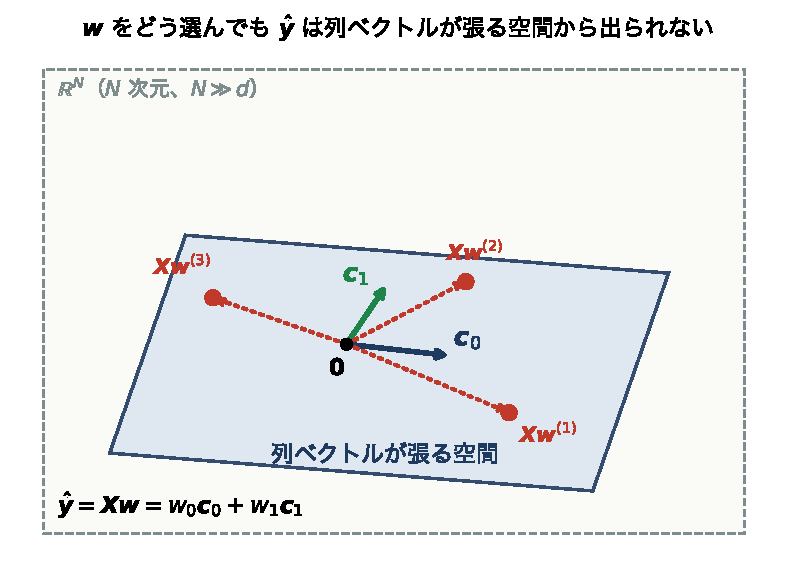
\includegraphics[width=0.72\linewidth]{figures/ch3_colspace_sweep}
  \caption{$\bm{w}$ を動かしたときの予測 $\hat{\bm{y}} = \bm{X}\bm{w}$ の動く範囲。
  $\bm{w}$ をどう選んでも $\hat{\bm{y}}$ は列ベクトルの張る部分空間から出られない。
  図は $\mathrm{rank}(\bm{X}) = 2$ の場合（平面）を描いた模式図である。}
  \label{fig:colspace-sweep}
\end{figure}

\subsubsection{列空間}

パラメータ $\bm{w}$ は $\mathbb{R}^{d+1}$ を自由に動ける。
そこで、$\bm{w}$ を動かしたときに $\hat{\bm{y}} = \bm{X}\bm{w}$ が取りうる値の全体を考える。

\begin{itembox}[l]{定義：列空間}
行列 $\bm{X} \in \mathbb{R}^{N \times (d+1)}$ に対して、
\begin{equation}
  \mathrm{Col}(\bm{X}) = \{\, \bm{X}\bm{w} \mid \bm{w} \in \mathbb{R}^{d+1} \,\} \subseteq \mathbb{R}^N
  \label{eq:colspace}
\end{equation}
を $\bm{X}$ の\textbf{列空間}（column space）または\textbf{値域}（range）と呼ぶ。
式\eqref{eq:pred-col}より、これは
\textbf{$\bm{X}$ の列ベクトルのすべての線形結合からなる集合}である。
\end{itembox}

記法を確認しておく（第1.2節参照）。$\{\, \cdots \mid \cdots \,\}$ の縦棒は「ただし」と読み、
左側に\textbf{集める要素の形}、右側に\textbf{その要素を作り出す変数の動く範囲}を書く。
したがって式\eqref{eq:colspace}は
「$\bm{w}$ が $\mathbb{R}^{d+1}$ 全体を動くとき、$\bm{X}\bm{w}$ という形のベクトルを
すべて集めた集合」と読む。
集めている要素は $\bm{w}$ ではなく $\bm{X}\bm{w} \in \mathbb{R}^N$ である点に注意する。
$\bm{w}$ は $\mathbb{R}^{d+1}$ の点、$\bm{X}\bm{w}$ は $\mathbb{R}^N$ の点であり、
$\mathrm{Col}(\bm{X})$ は後者の住む空間 $\mathbb{R}^N$ の部分集合である。

列空間は $\mathbb{R}^N$ の\textbf{部分空間}（subspace）である。
すなわち、$\bm{0}$ を含み、和とスカラー倍について閉じている：
$\bm{X}\bm{w}_1 + \bm{X}\bm{w}_2 = \bm{X}(\bm{w}_1 + \bm{w}_2) \in \mathrm{Col}(\bm{X})$、
$c\,\bm{X}\bm{w} = \bm{X}(c\bm{w}) \in \mathrm{Col}(\bm{X})$ が成り立つからである。

\subsubsection{仮説空間の正体}

ここで第1回を思い出そう。仮説空間 $\mathcal{H}$ は「候補となる関数の集合」という
抽象的な定義であった。しかし\textbf{訓練データ上での振る舞いだけ}に着目すれば、
仮説 $h(\cdot\,; \bm{w})$ は $N$ 次元ベクトル $\hat{\bm{y}} = \bm{X}\bm{w}$ と同一視できる。
したがって
\begin{equation}
  \{\, \hat{\bm{y}} \mid h(\cdot\,;\bm{w}) \in \mathcal{H} \,\} = \mathrm{Col}(\bm{X})
\end{equation}
となる。すなわち\textbf{線形モデルの仮説空間の正体は、計画行列の列空間である}。

この事実は重要な帰結をもたらす。
真の値のベクトル $\bm{y} \in \mathbb{R}^N$ は、一般に列空間の\textbf{外}にある。
なぜなら $\mathrm{Col}(\bm{X})$ は高々 $d+1$ 次元であるのに対し、
$\bm{y}$ は $N$ 次元空間の任意の点でありうるからである（通常 $N \gg d$）。
どれほど $\bm{w}$ を調整しても、予測は列空間の中しか動けない。
したがって
\begin{equation}
  \min_{\bm{w}} \|\bm{y} - \bm{X}\bm{w}\|
  = \text{（$\bm{y}$ から列空間までの距離）}
\end{equation}
であり、これを達成する $\hat{\bm{y}}$ は
\textbf{$\bm{y}$ の列空間への正射影}にほかならない。
\begin{figure}[H]
  \centering
  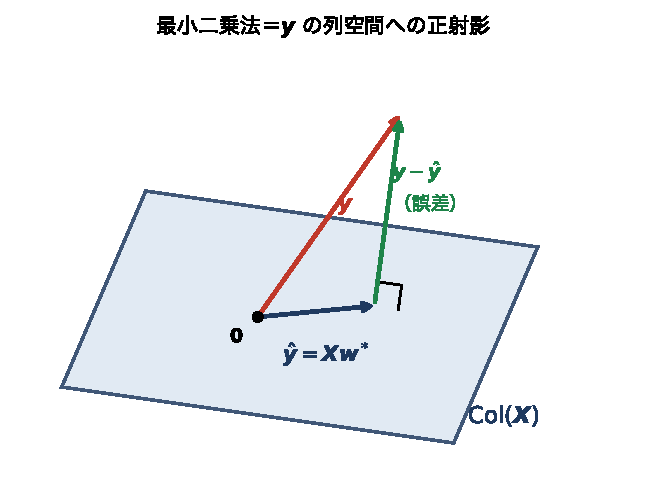
\includegraphics[width=0.66\linewidth]{figures/ch3_colspace}
  \caption{列空間と最小二乗法。予測 $\bm{X}\bm{w}$ は列空間の中しか動けないため、誤差を最小にするのは $\bm{y}$ を列空間へ正射影した点である。}
  \label{fig:colspace}
\end{figure}

第2回で学んだ正射影が、ここで再び現れる。
第4回ではこの幾何学的描像から\textbf{正規方程式}（normal equation）を導く。
これは「誤差ベクトル $\bm{y} - \bm{X}\bm{w}$ が列空間のすべての列と直交する」
という条件 $\bm{X}^\top (\bm{y} - \bm{X}\bm{w}) = \bm{0}$ を整理した
\begin{equation}
  \bm{X}^\top \bm{X} \bm{w} = \bm{X}^\top \bm{y}
  \label{eq:normal-intro}
\end{equation}
のことであり、最適なパラメータ $\bm{w}^*$ が
\textbf{連立一次方程式を解くだけで求まる}ことを意味する。

\subsubsection{ランク}

列空間の「大きさ」を測る量がランクである。

\begin{itembox}[l]{定義：ランク}
行列 $\bm{A}$ の列空間の次元を $\bm{A}$ の\textbf{ランク}（rank、階数）と呼び、
$\mathrm{rank}(\bm{A})$ と書く。
これは、$\bm{A}$ の列ベクトルのうち\textbf{線形独立}なものの最大個数に等しい。
\end{itembox}

線形独立の定義は第3.2.3項で与えた
（式\eqref{eq:lin-indep}、すなわち\textbf{どの列も他の列の線形結合で表せない}こと）。
そこで見たとおり、線形独立な列が $r$ 本あれば張られる空間は $r$ 次元になる。
ランクとは、まさにこの $r$ のことである。
図\ref{fig:colspace-sweep}で平面として描いたのは $\mathrm{rank}(\bm{X}) = 2$ の場合であり、
一般には $\mathrm{rank}(\bm{X})$ 次元の部分空間になる。

$\bm{X} \in \mathbb{R}^{N \times (d+1)}$ に対して、常に
$\mathrm{rank}(\bm{X}) \leq \min(N, d+1)$ が成り立つ。
等号が成り立つとき\textbf{フルランク}（full rank）であるという。

\subsubsection{ランク落ちと多重共線性}

$\mathrm{rank}(\bm{X}) < d+1$ となる場合、すなわち列が線形従属な場合を考えよう。
このとき、ある $\bm{v} \neq \bm{0}$ が存在して $\bm{X}\bm{v} = \bm{0}$ となる。
したがって任意の $\bm{w}$ に対して
\begin{equation}
  \bm{X}(\bm{w} + \bm{v}) = \bm{X}\bm{w} + \bm{X}\bm{v} = \bm{X}\bm{w}
  \label{eq:rank-shift}
\end{equation}
となり、\textbf{異なるパラメータが全く同じ予測を与える}。
すなわち最適なパラメータ $\bm{w}^*$ が一意に定まらない。

これは実データで頻繁に起こる。例えば、物件の広さを
「平方メートル」と「坪」の2つの列として記録した場合、
$\bm{c}_{\text{坪}} = 0.3025\,\bm{c}_{\text{m}^2}$ という関係があり、完全に線形従属である。
より一般に、複数の特徴が強く相関している状況を
\textbf{多重共線性}（multicollinearity）と呼ぶ。
相関するのは\textbf{列どうし}、すなわち特徴どうしである点に注意する。
行は個々のデータに対応しており、似た物件が何件あっても
$\mathrm{rank}(\bm{X}) \leq d+1$ という上限は変わらない。
問題になるのは「$\bm{c}_i$ と $\bm{c}_j$ が似ている」という列の間の関係である。

厳密に線形従属でなくとも、ほぼ従属であればパラメータの推定は極めて不安定になり、
データのわずかな変化で $\bm{w}^*$ が大きく変動する。
次の例でそれを確かめよう。

\subsubsubsection{例：ほぼ線形従属な2つの特徴}

$N = 4$ 件の物件について、家賃を予測する問題を考える。
\begin{itemize}
  \item 出力 $y$：\textbf{家賃}（万円）
  \item 特徴1：広さ（$\mathrm{m}^2$）
  \item 特徴2：部屋数（室）
\end{itemize}
すなわち $d = 2$ であり、計画行列は $\bm{X} \in \mathbb{R}^{4 \times 3}$ となる。
その3本の列はそれぞれ
\begin{align*}
  \bm{c}_0 &= (1,\; 1,\; 1,\; 1)^\top && \text{バイアス項のための定数列} \\
  \bm{c}_1 &= (22,\; 38,\; 61,\; 79)^\top && \text{4件の広さ（$\mathrm{m}^2$）} \\
  \bm{c}_2 &= (1,\; 2,\; 3,\; 4)^\top && \text{4件の部屋数（室）}
\end{align*}
であり、これらを並べると
\begin{equation*}
  \bm{X} = \begin{pmatrix}
    1 & 22 & 1 \\
    1 & 38 & 2 \\
    1 & 61 & 3 \\
    1 & 79 & 4
  \end{pmatrix}
\end{equation*}
となる。各行が1件の物件であり、例えば第3行は「広さ $61\,\mathrm{m}^2$、3室」の物件を表す。

部屋数が多ければ広さも大きいので、この2列は強く相関する：
\begin{equation*}
  \bm{c}_1 \approx 20\,\bm{c}_2
\end{equation*}
実際 $20\,\bm{c}_2 = (20, 40, 60, 80)^\top$ であり、
$\bm{c}_1 = (22, 38, 61, 79)^\top$ とのずれは各成分 $2$ 以内にすぎない。
ただし厳密には $\bm{c}_1 \neq 20\,\bm{c}_2$ なので $\mathrm{rank}(\bm{X}) = 3$、
すなわちフルランクであり、解は数学的には一意に定まる。

それでも困ったことが起こる。次の2つのパラメータを比べてみよう。
\begin{align*}
  \bm{w}^{(\mathrm{A})} &= (0,\; 0.5,\; 0)^\top
    &&\Rightarrow\quad \hat{\bm{y}} = (11,\; 19,\; 30.5,\; 39.5)^\top \\
  \bm{w}^{(\mathrm{B})} &= (0,\; 0,\; 10)^\top
    &&\Rightarrow\quad \hat{\bm{y}} = (10,\; 20,\; 30,\; 40)^\top
\end{align*}
$\bm{w}^{(\mathrm{A})}$ は「広さ $1\,\mathrm{m}^2$ につき $0.5$ 万円、部屋数は家賃に無関係」、
$\bm{w}^{(\mathrm{B})}$ は「部屋数1室につき $10$ 万円、広さは家賃に無関係」という、
\textbf{解釈が正反対のモデル}である。
にもかかわらず、予測はどのデータでも $1$ 万円以内しか違わない。

\subsubsubsection{なぜ2つの差を見るのか}
式\eqref{eq:rank-shift}が示していたのは
「$\bm{X}\bm{v} = \bm{0}$ を満たす方向 $\bm{v}$ に沿って $\bm{w}$ をずらしても予測は変わらない」
ということであった。
つまり2つのパラメータが同じ予測を与えるかどうかは、
\textbf{その差がそのような方向を向いているか}で決まる。
そこで差を計算すると
\begin{equation*}
  \bm{w}^{(\mathrm{B})} - \bm{w}^{(\mathrm{A})} = (0,\; -0.5,\; 10)^\top
  = -0.5\,\bm{v}, \qquad \bm{v} = (0,\; 1,\; -20)^\top
\end{equation*}
となる。この $\bm{v}$ は、まさに $\bm{c}_1 \approx 20\,\bm{c}_2$ という列どうしの関係を
係数の形で書いたものである。実際
\begin{equation*}
  \bm{X}\bm{v} = 0\cdot\bm{c}_0 + 1\cdot\bm{c}_1 - 20\cdot\bm{c}_2
  = \begin{pmatrix} 22 \\ 38 \\ 61 \\ 79 \end{pmatrix}
  - \begin{pmatrix} 20 \\ 40 \\ 60 \\ 80 \end{pmatrix}
  = \begin{pmatrix} 2 \\ -2 \\ 1 \\ -1 \end{pmatrix}
\end{equation*}
であり、2つの列がほぼ打ち消し合っている。

\subsubsubsection{なぜ $\bm{X}\bm{v}$ が「$\bm{0}$ に近い」といえるのか}
まず、$\bm{0}$ に近いといっているのが\textbf{どのベクトルか}を確認する。
近いのは $\bm{v}$ ではなく、その像 $\bm{X}\bm{v}$ の方である。
実際 $\bm{v} = (0,\; 1,\; -20)^\top$ 自身は $\|\bm{v}\| = \sqrt{401} \approx 20.0$ であり、
決して小さなベクトルではない。
\begin{itemize}
  \item $\bm{v} \in \mathbb{R}^{3}$：\textbf{パラメータの空間}の点。$\bm{w}$ をずらす向きを表す
  \item $\bm{X}\bm{v} \in \mathbb{R}^{4}$：\textbf{予測の空間}の点。
        そのずらしによって予測 $\hat{\bm{y}}$ がどれだけ変わるかを表す
\end{itemize}
「予測がほとんど変わらない」と言いたいのだから、小ささを問題にすべきは後者、
すなわち $\bm{X}\bm{v}$ である。

その上で、ベクトルが「小さい」かどうかは、\textbf{何と比べるか}を決めなければ意味をもたない。
そこで、$\bm{w}$ を\textbf{同じ長さだけ}動かしたときの予測の変化量を比べる。
$\|\bm{v}\| = \sqrt{1 + 400} \approx 20.0$ なので、
同じ長さをもつ別の方向として $\bm{u} = (0,\; 20,\; 0)^\top$（$\|\bm{u}\| = 20$）をとると
\begin{align*}
  \bm{X}\bm{u} &= 20\,\bm{c}_1 = (440,\; 760,\; 1220,\; 1580)^\top,
    & \|\bm{X}\bm{u}\| &\approx 2181 \\
  \bm{X}\bm{v} &= (2,\; -2,\; 1,\; -1)^\top,
    & \|\bm{X}\bm{v}\| &= \sqrt{10} \approx 3.2
\end{align*}
となる。すなわち、$\bm{w}$ を同じ距離だけ動かしても、
$\bm{v}$ の向きに動かしたときの予測の変化は他の向きの約 $700$ 分の1でしかない。
この意味で $\bm{X}\bm{v}$ は $\bm{0}$ に近い。

\subsubsubsection{損失関数の形で見る：ほぼ平らな谷}

ここが多重共線性のいちばん重要な点なので、経験損失の形として見ておこう。

完全に線形従属なら $\bm{X}\bm{v}$ はちょうど $\bm{0}$ になり、
この方向に $\bm{w}$ を動かしても予測は\textbf{まったく}変わらない（式\eqref{eq:rank-shift}）。
ほぼ従属な今の場合は、まったくではないがほとんど変わらない。
予測が変わらなければ経験損失 $L_D(\bm{w}) = \frac{1}{N}\|\bm{y} - \bm{X}\bm{w}\|^2$ も変わらない。
すなわち $L_D$ は $\bm{v}$ の方向に\textbf{ほぼ平らな谷}になっている
（図\ref{fig:flat-valley}左）。
解釈が正反対の $\bm{w}^{(\mathrm{A})}$ と $\bm{w}^{(\mathrm{B})}$ が同程度に良い解に見えたのは、
2点がこの谷の底に並んでいたからである。

\begin{figure}[H]
  \centering
  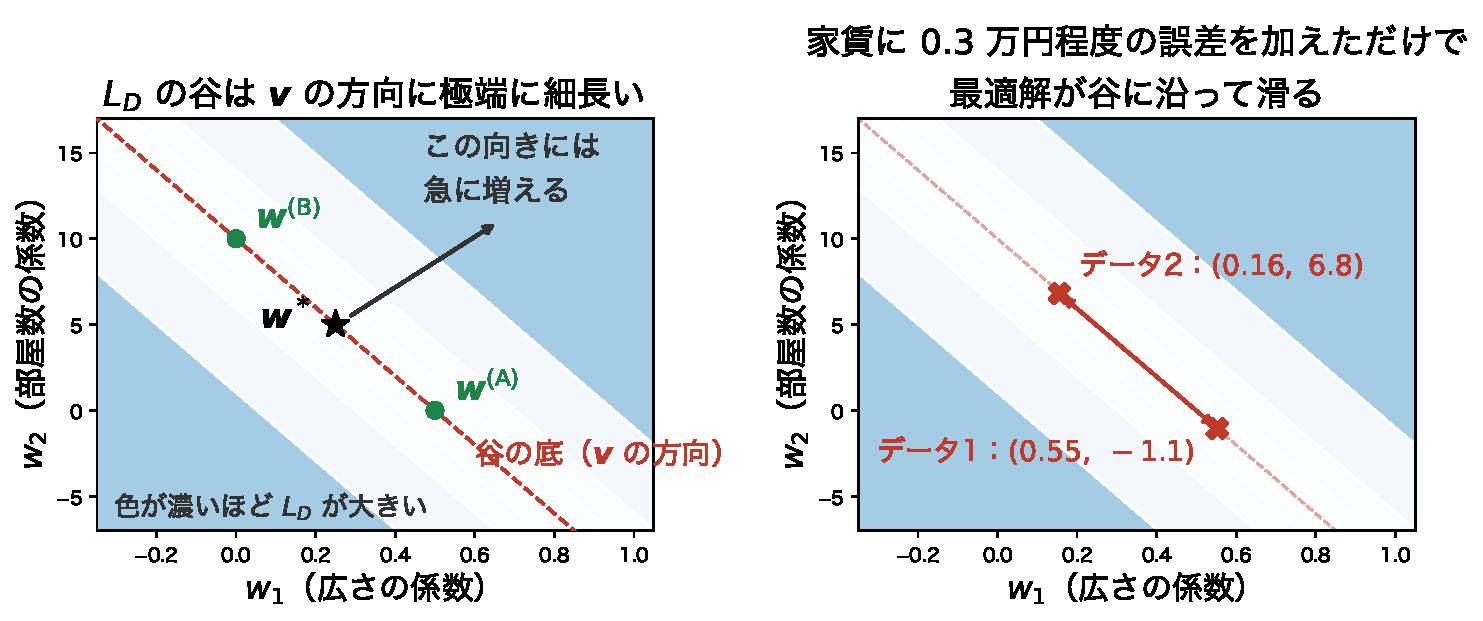
\includegraphics[width=\linewidth]{figures/ch3_flat_valley}
  \caption{ほぼ平らな谷。左：経験損失 $L_D$ の等高線。$\bm{v} = (0,1,-20)^\top$ の方向には
  ほとんど増えず、それと交わる向きには急に増える。
  右：家賃に $0.3$ 万円程度の誤差を加えた2通りのデータについて最適解を求めたもの。
  谷に沿って大きく離れ、「広さ中心のモデル」と「部屋数中心のモデル」のどちらにもなりうる。
  なお縦軸と横軸で目盛りの刻みが異なるため、谷の細さは実際よりも緩やかに見えている。}
  \label{fig:flat-valley}
\end{figure}

谷が平らであることの帰結は深刻である。
手元のデータがわずかに違えば、谷の底のどこで最小値を取るかは簡単に入れ替わる。
図\ref{fig:flat-valley}右は、家賃に $0.3$ 万円程度の誤差を加えた2通りのデータについて
最適解を求めたものである。
得られる $\bm{w}^*$ は谷に沿って大きく滑り、
「広さが効いている」とも「部屋数が効いている」とも結論できてしまう。
これが\textbf{推定が不安定になる}ということの正体である。

なお、谷の\textbf{向き}と\textbf{細さ}は計画行列 $\bm{X}$ だけで決まる。
図を描くには家賃の実測値 $\bm{y}$ が必要だが、$\bm{y}$ を変えても
谷の\textbf{底の位置}が動くだけで、谷の細長さそのものは変わらない。
多重共線性は $\bm{X}$ の性質であり、出力がどのような値であっても同じ不安定さが生じる。

\textbf{解の一意性を回復し、推定を安定させる}ことが、
第6回で学ぶ\textbf{正則化}の重要な役割の一つである。
第1回で見た「仮説空間が大きすぎると過学習する」という問題と、
ここで見た「列が従属だと解が定まらない」という問題は、
いずれも\textbf{モデルの自由度が過剰である}ことに由来しており、
正則化はその両方に効く処方箋となる。

\subsubsection{数値例}

3件のデータについて、特徴を「広さ（$\mathrm{m}^2$）」と「広さ（坪）」とした場合の計画行列
\begin{equation*}
  \bm{X} = \begin{pmatrix} 1 & 20 & 6 \\ 1 & 40 & 12 \\ 1 & 60 & 18 \end{pmatrix}
\end{equation*}
を考える。第3列は第2列の $0.3$ 倍であり、線形従属である。
実際、$\bm{v} = (0, 0.3, -1)^\top$ とすると
\begin{equation*}
  \bm{X}\bm{v} = 0 \cdot \bm{c}_0 + 0.3\,\bm{c}_1 - 1 \cdot \bm{c}_2
  = \begin{pmatrix} 6 \\ 12 \\ 18 \end{pmatrix} - \begin{pmatrix} 6 \\ 12 \\ 18 \end{pmatrix}
  = \bm{0}
\end{equation*}
となる。よって $\mathrm{rank}(\bm{X}) = 2 < 3$ であり、
$\bm{w}^*$ に $\bm{v}$ の任意の定数倍を加えても予測は変わらない。
この場合、列空間は $\mathbb{R}^3$ の中の2次元平面であり、
3次元空間全体を張ることはできない。


\subsection{行列のノルム}

第2回では、ベクトルの「大きさ」をノルム $\|\bm{x}\| = \sqrt{\bm{x}^\top \bm{x}}$ で測った。
行列に対しても同様に大きさを測りたい場面がある。
最も基本的なものが\textbf{フロベニウスノルム}である。

\subsubsection{定義}

\begin{itembox}[l]{定義：フロベニウスノルム}
行列 $\bm{A} \in \mathbb{R}^{m \times n}$ に対して、
\begin{equation}
  \|\bm{A}\|_F = \sqrt{\sum_{i=1}^{m} \sum_{j=1}^{n} a_{ij}^2}
\end{equation}
を $\bm{A}$ の\textbf{フロベニウスノルム}（Frobenius norm）と呼ぶ。
添字の $F$ は Frobenius の頭文字である。
\end{itembox}

定義を見ればわかるとおり、これは\textbf{行列の全成分を1本のベクトルとみなしたときの
ユークリッドノルム}にほかならない。
実際、$m \times n$ 行列の成分を順に並べて $mn$ 次元ベクトルを作れば、
そのノルムが $\|\bm{A}\|_F$ である。
したがって、第2回で示したノルムの3性質（非負性・斉次性・三角不等式）は
そのまま成り立つ。

例えば
\begin{equation*}
  \bm{A} = \begin{pmatrix} 1 & 2 \\ -2 & 4 \end{pmatrix}
  \quad \Longrightarrow \quad
  \|\bm{A}\|_F = \sqrt{1^2 + 2^2 + (-2)^2 + 4^2} = \sqrt{25} = 5
\end{equation*}
である。

\subsubsection{列ベクトルとの関係}

$\bm{A}$ の列を $\bm{c}_1, \ldots, \bm{c}_n$ とすると、
二重和を列ごとにまとめることで
\begin{equation}
  \|\bm{A}\|_F^2 = \sum_{j=1}^{n} \sum_{i=1}^{m} a_{ij}^2 = \sum_{j=1}^{n} \|\bm{c}_j\|^2
\end{equation}
が得られる。すなわち\textbf{フロベニウスノルムの二乗は、各列ベクトルのノルムの二乗和}である。
行についても同様である。

また、トレース（正方行列の対角成分の和）$\mathrm{tr}(\bm{B}) = \sum_i b_{ii}$ を用いると
\begin{equation}
  \|\bm{A}\|_F^2 = \mathrm{tr}(\bm{A}^\top \bm{A})
\end{equation}
と書ける。実際、$(\bm{A}^\top\bm{A})_{jj} = \sum_i a_{ij}^2 = \|\bm{c}_j\|^2$ であり、
その和をとれば前式に一致する。
この表現は、第4回以降で行列の微分を扱う際に有用である。

\subsubsection{どのような場面で使うか}

フロベニウスノルムは、機械学習において主に次の3つの場面で用いられる。

\paragraph{(1) 正則化：モデルの複雑さを測る}
第1回で見たように、仮説空間が大きすぎると過学習が生じる。
第6回で学ぶ\textbf{L2正則化}は、パラメータの大きさを罰則として加えることで
これを抑制する。線形モデルでは経験損失に $\lambda \|\bm{w}\|^2$ を加えるが、
ニューラルネットワークのようにパラメータが行列 $\bm{W}$ である場合は、
\begin{equation}
  \min_{\bm{W}} \; \left\{ L_D(\bm{W}) + \lambda \|\bm{W}\|_F^2 \right\}
\end{equation}
とフロベニウスノルムを用いる。これは\textbf{重み減衰}（weight decay）と呼ばれ、
深層学習で標準的に使われる手法である。
「重みを不必要に大きくしない」という要請を、行列の大きさとして数式化したものである。

\paragraph{(2) 行列の近さを測る：低ランク近似}
2つの行列がどれだけ近いかは、差のフロベニウスノルム $\|\bm{A} - \bm{B}\|_F$ で測る。
第2回でベクトルの距離を $\|\bm{x} - \bm{y}\|$ で測ったのと同じ考え方である。

特に重要なのが\textbf{低ランク近似}である。
前節で見たように、ランクは列空間の次元、すなわちデータの「実質的な自由度」を表す。
そこで、与えられた行列 $\bm{A}$ を、ランクが $r$ 以下の行列 $\bm{B}$ で近似する問題
\begin{equation}
  \min_{\mathrm{rank}(\bm{B}) \leq r} \|\bm{A} - \bm{B}\|_F
\end{equation}
を考える。この解は特異値分解によって与えられることが知られている。
主成分分析による次元削減、推薦システムにおける行列分解、
大規模言語モデルの効率的な微調整手法である LoRA などは、
いずれもこの考え方に基づいている。

\paragraph{(3) 収束判定と勾配の大きさ}
第5回で学ぶ勾配降下法のような反復計算では、
更新の前後でパラメータがほとんど変化しなくなった時点で計算を止める。
このとき $\|\bm{W}^{(t+1)} - \bm{W}^{(t)}\|_F < \varepsilon$ を判定条件に用いる。
また、深層学習では勾配が発散することを防ぐため、
勾配のノルムが一定値を超えたら縮小する
\textbf{勾配クリッピング}（gradient clipping）という手法が用いられるが、
ここでもフロベニウスノルムが使われる。

\subsubsection{他の行列ノルムとの違い}

行列のノルムはフロベニウスノルムだけではない。代表的なものに
\textbf{スペクトルノルム}（作用素ノルム）
\begin{equation}
  \|\bm{A}\|_2 = \max_{\bm{x} \neq \bm{0}} \frac{\|\bm{A}\bm{x}\|}{\|\bm{x}\|}
\end{equation}
がある。これは「行列がベクトルを最大何倍に引き伸ばすか」を表す量であり、
線形写像としての性質を測る。両者の間には
$\|\bm{A}\|_2 \leq \|\bm{A}\|_F$ という関係がある。

目的に応じた使い分けを簡単にまとめる。
\begin{itemize}
  \item \textbf{フロベニウスノルム}：成分の大きさの総量を測りたいとき（正則化、近似誤差）。
    計算が容易で微分しやすい
  \item \textbf{スペクトルノルム}：変換としての増幅率を抑えたいとき
    （安定性の解析、GANのSpectral Normalizationなど）
\end{itemize}
本講義で扱うのは主にフロベニウスノルムである。


\subsection{固有値と固有ベクトル（概念）}

最後に、行列のもう一つの重要な見方に触れる。本節は概念の紹介にとどめ、
詳細は第6回以降で必要に応じて扱う。

\begin{itembox}[l]{定義：固有値と固有ベクトル}
正方行列 $\bm{A} \in \mathbb{R}^{n \times n}$ に対して、
\begin{equation}
  \bm{A}\bm{v} = \lambda \bm{v}, \qquad \bm{v} \neq \bm{0}
\end{equation}
を満たす実数 $\lambda$ を\textbf{固有値}（eigenvalue）、
$\bm{v}$ を対応する\textbf{固有ベクトル}（eigenvector）と呼ぶ。
\end{itembox}

\subsubsection{幾何学的な意味}

行列は一般にベクトルの向きと長さの両方を変える（第3.3節）。
しかし固有ベクトルだけは\textbf{向きが変わらず、長さだけが $\lambda$ 倍される}。
すなわち固有ベクトルは、その線形変換の「軸」を表す
（図\ref{fig:eigen}左）。
$\lambda < 0$ のときは向きが逆になるが、同じ直線上にとどまる点は変わらない。

図\ref{fig:eigen}右のように、単位円を $\bm{A}$ で写すと楕円になる。
このとき\textbf{楕円の軸の向きが固有ベクトル、軸の長さが固有値}に対応する。
ただしこの描像が成り立つのは $\bm{A}$ が\textbf{対称行列}（$\bm{A}^\top = \bm{A}$）の場合である。
幸い、機械学習で固有値を考える相手は
$\bm{X}^\top\bm{X}$、共分散行列、ヘッセ行列のようにいずれも対称行列なので、
この「楕円の軸」という描像をそのまま使える。

\begin{figure}[htbp]
  \centering
  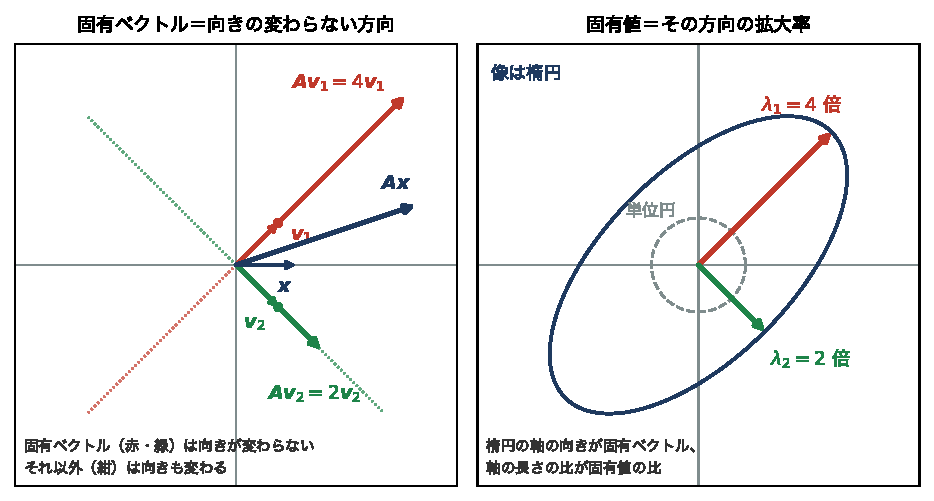
\includegraphics[width=\linewidth]{figures/ch3_eigen}
  \caption{$\bm{A} = \begin{pmatrix} 3 & 1 \\ 1 & 3 \end{pmatrix}$ による変換。
  左：固有ベクトル $\bm{v}_1, \bm{v}_2$ は向きが変わらず、長さだけがそれぞれ $4$ 倍、$2$ 倍になる。
  固有ベクトルでない $\bm{x}$ は向きまで変わる。
  右：単位円の像は楕円になり、楕円の軸の向きが固有ベクトル、軸の長さが固有値に対応する。}
  \label{fig:eigen}
\end{figure}

\subsubsection{特性方程式}

固有値を実際に求める方法を見ておく。
$\bm{I}_n$ を\textbf{単位行列}（identity matrix）、
すなわち対角成分がすべて $1$、それ以外が $0$ の $n \times n$ 行列とする。
任意の $\bm{x}$ に対して $\bm{I}_n \bm{x} = \bm{x}$ が成り立つ。
これを使うと定義式は
\begin{equation}
  \bm{A}\bm{v} = \lambda\bm{v}
  \;\Longleftrightarrow\;
  (\bm{A} - \lambda\bm{I}_n)\,\bm{v} = \bm{0}
  \label{eq:eigen-shift}
\end{equation}
と書き直せる。

ここで第3.5節の議論がそのまま効く。
式\eqref{eq:eigen-shift}が $\bm{v} \neq \bm{0}$ の解をもつということは、
\textbf{行列 $\bm{A} - \lambda\bm{I}_n$ の列が線形従属}だということである
（ランク落ちしている、ということに他ならない）。

$2 \times 2$ の場合、この条件は簡単に書ける。
$\bm{M} = \begin{pmatrix} a & b \\ c & d \end{pmatrix}$ の2本の列
$(a, c)^\top$ と $(b, d)^\top$ が平行であることと
\begin{equation}
  \det \bm{M} = ad - bc = 0
\end{equation}
は同値である。この量 $\det \bm{M}$ を\textbf{行列式}（determinant）と呼ぶ。
したがって固有値は
\begin{equation}
  \det(\bm{A} - \lambda\bm{I}_n) = 0
  \label{eq:char-eq}
\end{equation}
を満たす $\lambda$ として求まる。これを\textbf{特性方程式}（characteristic equation）と呼ぶ。

\subsubsubsection{例}

$\bm{A} = \begin{pmatrix} 3 & 1 \\ 1 & 3 \end{pmatrix}$ の固有値と固有ベクトルを求めよう。
特性方程式は
\begin{equation*}
  \det\!\begin{pmatrix} 3 - \lambda & 1 \\ 1 & 3 - \lambda \end{pmatrix}
  = (3 - \lambda)^2 - 1 = \lambda^2 - 6\lambda + 8 = (\lambda - 2)(\lambda - 4) = 0
\end{equation*}
であるから、固有値は $\lambda_1 = 4$, $\lambda_2 = 2$ である。
それぞれに対して式\eqref{eq:eigen-shift}を解くと
\begin{align*}
  \lambda_1 = 4:\quad
    \begin{pmatrix} -1 & 1 \\ 1 & -1 \end{pmatrix}\bm{v} = \bm{0}
    &\;\Rightarrow\; \bm{v}_1 = (1,\; 1)^\top \text{（の定数倍）} \\
  \lambda_2 = 2:\quad
    \begin{pmatrix} 1 & 1 \\ 1 & 1 \end{pmatrix}\bm{v} = \bm{0}
    &\;\Rightarrow\; \bm{v}_2 = (1,\; -1)^\top \text{（の定数倍）}
\end{align*}
を得る。実際に確かめると
$\bm{A}\bm{v}_1 = (4, 4)^\top = 4\,\bm{v}_1$、
$\bm{A}\bm{v}_2 = (2, -2)^\top = 2\,\bm{v}_2$ であり、
どちらも向きが変わらず長さだけが $\lambda$ 倍になっている。
これが図\ref{fig:eigen}で描いた状況である。
なお固有ベクトルは定数倍の自由度をもつので、
長さを $1$ に揃えて $\bm{v}_1 = (1,1)^\top/\sqrt{2}$ と書くことも多い。

\subsubsection{機械学習での現れ方}

機械学習では次のような場面で現れる（図\ref{fig:eigen-ml}）。
\begin{itemize}
  \item \textbf{主成分分析}：データの分散が最大となる方向が、共分散行列の最大固有値に対応する固有ベクトルである
  \item \textbf{最適化の収束}：第5回で扱う勾配降下法の収束の速さは、損失関数の曲がり具合（ヘッセ行列）の固有値の比で決まる
  \item \textbf{数値的安定性}：$\bm{X}^\top \bm{X}$ の最小固有値が $0$ に近いとき、多重共線性が生じており推定が不安定になる
\end{itemize}

3つはいずれも\textbf{「どの向きにどれだけ伸びているか」}を固有値と固有ベクトルで読んでいる点で共通している。

\begin{figure}[htbp]
  \centering
  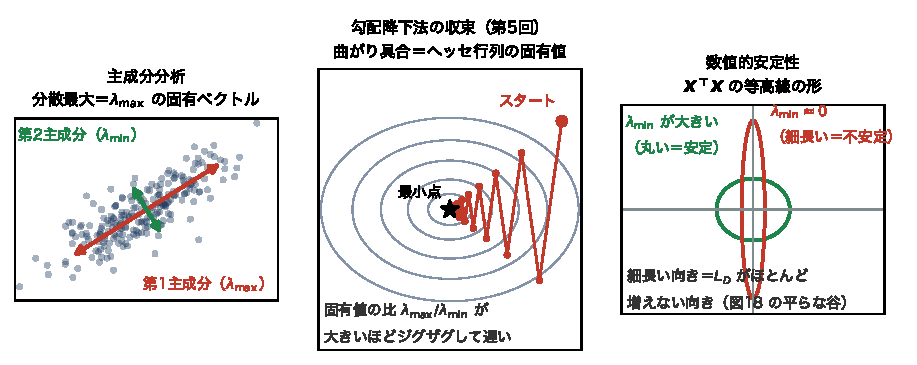
\includegraphics[width=\linewidth]{figures/ch3_eigen_ml}
  \caption{固有値が現れる3つの場面（概念図）。
  左：主成分分析。データが最も散らばる方向が共分散行列の最大固有値の固有ベクトルである。
  中：勾配降下法。等高線が細長い（固有値の比が大きい）ほど経路がジグザグし、収束が遅くなる。
  右：数値的安定性。$\bm{X}^\top\bm{X}$ の最小固有値が $0$ に近いほど等高線が細長くなり、
  その向きには $L_D$ がほとんど増えない。これが図\ref{fig:flat-valley}で見た「平らな谷」である。}
  \label{fig:eigen-ml}
\end{figure}

\subsubsection{ランクとの関係}

上の3番目の項目は、前節のランクの議論と直接つながっている。
実際、$\bm{X}^\top\bm{X}$ について次の3つは同値である：
\begin{enumerate}
  \item $\mathrm{rank}(\bm{X}) < d+1$（列が線形従属、多重共線性がある）
  \item $\bm{X}^\top\bm{X}$ が固有値 $0$ をもつ
  \item $\bm{X}^\top\bm{X}$ が半正定値だが正定値ではない
\end{enumerate}
第2回で述べたように、$\bm{X}^\top\bm{X}$ は常に半正定値である
（任意の $\bm{v}$ に対し $\bm{v}^\top \bm{X}^\top \bm{X} \bm{v} = \|\bm{X}\bm{v}\|^2 \geq 0$）。
正定値でない、すなわち $\bm{X}\bm{v} = \bm{0}$ となる $\bm{v} \neq \bm{0}$ が存在することが、
前節で見た「解が一意に定まらない」状況にほかならない。


\subsection{まとめ}

\begin{itemize}
  \item 行列は数を長方形に並べたものであり、線形写像と同一視できる
  \item 積 $\bm{A}\bm{x}$ には「行との内積」と「列の線形結合」の2つの見方がある
  \item $N$ 件のデータを積み上げた計画行列 $\bm{X}$ により、
    予測全体が $\hat{\bm{y}} = \bm{X}\bm{w}$、経験損失が $\frac{1}{N}\|\bm{y} - \bm{X}\bm{w}\|^2$ と書ける
  \item 予測 $\bm{X}\bm{w}$ は $\bm{X}$ の列の線形結合であり、
    その全体である列空間 $\mathrm{Col}(\bm{X})$ が線形モデルの仮説空間の正体である
  \item $\bm{y}$ は一般に列空間の外にあり、最小二乗法は $\bm{y}$ の列空間への正射影を求める問題である
  \item ランクは列空間の次元であり、ランクが落ちると（多重共線性）解が一意に定まらない
  \item フロベニウスノルム $\|\bm{A}\|_F$ は行列の大きさを測る。
    正則化（重み減衰）、行列の近さ（低ランク近似）、収束判定に用いられる
\end{itemize}

次回（第4回）は、本章で得た
$\min_{\bm{w}} \|\bm{y} - \bm{X}\bm{w}\|^2$ という定式化を出発点に、
最小二乗法を射影の幾何学として解き、正規方程式を導く。


\subsection{演習問題}

\begin{enumerate}
  \item \textbf{行列とベクトルの積}\quad
    \begin{equation*}
      \bm{A} = \begin{pmatrix} 2 & 0 & 1 \\ -1 & 3 & 2 \end{pmatrix}, \qquad
      \bm{x} = \begin{pmatrix} 1 \\ 2 \\ -1 \end{pmatrix}
    \end{equation*}
    とする。
    \begin{enumerate}
      \item $\bm{A}$ は何行何列の行列か。$\bm{A}\bm{x}$ は何次元のベクトルか。
      \item $\bm{A}\bm{x}$ を「行との内積」として計算せよ。
      \item $\bm{A}\bm{x}$ を「列の線形結合」として計算し、(b) と一致することを確認せよ。
      \item $\bm{A}^\top$ を書け。また $\bm{A}^\top$ は何行何列か。
    \end{enumerate}

  \item \textbf{線形写像}\quad
    \begin{enumerate}
      \item $f(\bm{x}) = \bm{A}\bm{x}$ が線形写像であること、
        すなわち $f(\bm{x}+\bm{y}) = f(\bm{x}) + f(\bm{y})$ と $f(c\bm{x}) = cf(\bm{x})$ を、
        行列とベクトルの積の定義から証明せよ。
      \item $g(\bm{x}) = \bm{A}\bm{x} + \bm{b}$（$\bm{b} \neq \bm{0}$）は線形写像でないことを、
        $g(\bm{0})$ を計算して示せ。このような写像を何と呼ぶか。
    \end{enumerate}

  \item \textbf{計画行列}\quad
    3軒の物件について、広さ（$\mathrm{m}^2$）と駅からの距離（分）が
    $(20, 5)$、$(35, 10)$、$(50, 3)$ であり、
    家賃（万円）が $12, 15, 20$ であるとする。
    \begin{enumerate}
      \item バイアス項を含む計画行列 $\bm{X}$ と、目的変数のベクトル $\bm{y}$ を書け。
      \item $\bm{X}$ は何行何列か。また、行と列はそれぞれ何を表すか。
      \item $\bm{w} = (3, 0.5, -0.3)^\top$ のとき、予測ベクトル $\hat{\bm{y}} = \bm{X}\bm{w}$ を求めよ。
      \item この $\bm{w}$ に対する経験損失 $\frac{1}{N}\|\bm{y} - \bm{X}\bm{w}\|^2$ を求めよ。
    \end{enumerate}

  \item \textbf{列空間}\quad
    \begin{equation*}
      \bm{X} = \begin{pmatrix} 1 & 2 \\ 1 & 4 \\ 1 & 6 \end{pmatrix}
    \end{equation*}
    とする。
    \begin{enumerate}
      \item $\mathrm{Col}(\bm{X})$ の要素を、$\bm{w} = (w_0, w_1)^\top$ を用いて具体的に書き下せ。
      \item $\mathrm{Col}(\bm{X})$ は $\mathbb{R}^3$ の中でどのような図形か。その次元はいくつか。
      \item $\bm{y} = (1, 2, 4)^\top$ は $\mathrm{Col}(\bm{X})$ に属するか。
        属さない場合、それは何を意味するか。
    \end{enumerate}

  \item \textbf{ランクと多重共線性}\quad
    \begin{equation*}
      \bm{X} = \begin{pmatrix} 1 & 2 & 4 \\ 1 & 3 & 6 \\ 1 & 5 & 10 \end{pmatrix}
    \end{equation*}
    とする。
    \begin{enumerate}
      \item 第3列と第2列の関係を述べよ。
      \item $\bm{X}\bm{v} = \bm{0}$ を満たす $\bm{v} \neq \bm{0}$ を1つ求めよ。
      \item $\mathrm{rank}(\bm{X})$ を求めよ。
      \item $\bm{w}^* = (1, 2, 1)^\top$ が経験損失を最小にするとき、
        同じ予測を与える別のパラメータを1つ挙げよ。
        この事実は、最適なパラメータの一意性について何を意味するか。
    \end{enumerate}

  \item \textbf{仮説空間と列空間}\quad
    $N$ 件のデータに対する線形モデルを考える。
    \begin{enumerate}
      \item $N = 100$、$d = 3$（バイアス項を含めて4列）のとき、
        $\mathrm{Col}(\bm{X})$ は $\mathbb{R}^{100}$ の中の高々何次元の部分空間か。
      \item 真の値のベクトル $\bm{y} \in \mathbb{R}^{100}$ が
        $\mathrm{Col}(\bm{X})$ に属さないとき、経験損失を $0$ にできるか。理由とともに述べよ。
      \item 第1回の問7では「$N$ 個のデータ点に対し $M = N-1$ 次の多項式なら経験損失を $0$ にできる」
        ことを見た。この事実を、列空間の次元という観点から説明せよ。
    \end{enumerate}

  \item \textbf{フロベニウスノルム}\quad
    \begin{equation*}
      \bm{A} = \begin{pmatrix} 3 & 0 \\ 4 & 12 \end{pmatrix}, \qquad
      \bm{B} = \begin{pmatrix} 3 & 1 \\ 4 & 12 \end{pmatrix}
    \end{equation*}
    とする。
    \begin{enumerate}
      \item $\|\bm{A}\|_F$ を求めよ。
      \item $\bm{A}$ の各列のノルム $\|\bm{c}_1\|, \|\bm{c}_2\|$ を求め、
        $\|\bm{A}\|_F^2 = \|\bm{c}_1\|^2 + \|\bm{c}_2\|^2$ が成り立つことを確認せよ。
      \item $\|\bm{A} - \bm{B}\|_F$ を求めよ。この値は何を意味するか。
      \item $\mathrm{tr}(\bm{A}^\top \bm{A})$ を計算し、$\|\bm{A}\|_F^2$ と一致することを確認せよ。
      \item ニューラルネットワークの学習において
        $L_D(\bm{W}) + \lambda \|\bm{W}\|_F^2$ を最小化することの意味を、
        $\lambda$ を大きくした場合に $\bm{W}$ がどうなるかとあわせて説明せよ。
    \end{enumerate}

  \item \textbf{行列の積と内積}\quad
    \begin{equation*}
      \bm{A} = \begin{pmatrix} 1 & 0 \\ 0 & 1 \end{pmatrix} \in \mathbb{R}^{2 \times 2},
      \qquad
      \bm{B} = \begin{pmatrix} 1 & 2 & 0 \\ 1 & 0 & 3 \end{pmatrix} \in \mathbb{R}^{2 \times 3}
    \end{equation*}
    とする。
    \begin{enumerate}
      \item 積 $\bm{A}\bm{B}$ は何行何列の行列か。また、積 $\bm{B}\bm{A}$ は定義されるか。
      \item $\bm{A}$ の第 $i$ 行を $\bm{r}_i^\top$、$\bm{B}$ の第 $j$ 列を $\bm{c}_j$ とするとき、
        $(\bm{A}\bm{B})_{ij} = \bm{r}_i^\top \bm{c}_j$ が成り立つことを、
        行列の積の定義 $(\bm{A}\bm{B})_{ij} = \sum_{k} a_{ik} b_{kj}$ から示せ。
      \item $\bm{A}\bm{B}$ を計算せよ。$6$ 個の成分がそれぞれどの行とどの列の内積か明記すること。
      \item $\bm{B}^\top \bm{A}^\top$ を計算し、$(\bm{A}\bm{B})^\top$ と一致することを確認せよ。
    \end{enumerate}

  \item \textbf{固有値と固有ベクトル}\quad
    \begin{equation*}
      \bm{A} = \begin{pmatrix} 2 & 1 \\ 1 & 2 \end{pmatrix},
      \qquad
      \bm{B} = \begin{pmatrix} 1 & 2 \\ 2 & 4 \end{pmatrix}
    \end{equation*}
    とする。
    \begin{enumerate}
      \item $\bm{A}$ の特性方程式 $\det(\bm{A} - \lambda\bm{I}_2) = 0$ を書き下し、
        固有値 $\lambda_1 > \lambda_2$ を求めよ。
      \item 各固有値に対応する固有ベクトルを1つずつ求めよ。
      \item (b) で求めた固有ベクトル $\bm{v}$ について $\bm{A}\bm{v}$ を実際に計算し、
        向きが変わらず長さが $\lambda$ 倍になっていることを確認せよ。
      \item $\bm{B}$ の固有値を求めよ。固有値 $0$ をもつことを確認し、
        それが $\mathrm{rank}(\bm{B})$ および $\bm{B}$ の列の線形従属性と
        どう対応しているかを説明せよ。
      \item (d) の固有値 $0$ に対応する固有ベクトル $\bm{v}$ を求め、
        $\bm{B}\bm{v} = \bm{0}$ を確認せよ。
        第3.5.5項の議論に照らして、この $\bm{v}$ が何を意味するかを述べよ。
    \end{enumerate}
\end{enumerate}



%===========================================
% Chapter 4
%===========================================
\section{最小二乗法（幾何学）}

第3回では、$N$ 件のデータに対する予測が $\hat{\bm{y}} = \bm{X}\bm{w}$ と書けること、
そして経験損失が $L_D(\bm{w}) = \frac{1}{N}\|\bm{y} - \bm{X}\bm{w}\|^2$ という
一つの式にまとまることを見た。
また、予測が計画行列の\textbf{列空間}の中しか動けないこと、
したがって最良の予測は $\bm{y}$ をその列空間へ\textbf{正射影}した点であることも確認した。

本章では、この描像から出発して、最適なパラメータ $\bm{w}^*$ を実際に求める。
導出は\textbf{2通り}行う。一つは幾何学（射影）による導出、
もう一つは微分による導出である。
この2つはまったく違う見た目をしているが、同じ式にたどり着く。
その式が\textbf{正規方程式}である。

さらに本章では、解が一意に定まる条件、
一意に定まらないときにどう扱うか（\textbf{擬似逆行列}）、
そして実際に計算機で解くときの注意までを扱う。


\subsection{問題の確認}

\subsubsection{これまでの到達点}

第3回の結論を再掲する。$N$ 件のデータに対する予測と経験損失は
\begin{equation}
  \hat{\bm{y}} = \bm{X}\bm{w} \in \mathbb{R}^N, \qquad
  L_D(\bm{w}) = \frac{1}{N}\|\bm{y} - \bm{X}\bm{w}\|^2
  \label{eq:ch4-setup}
\end{equation}
であった（式\eqref{eq:lsq-matrix}）。ここで
$\bm{X} \in \mathbb{R}^{N \times (d+1)}$ は計画行列、
$\bm{y} \in \mathbb{R}^N$ は真の値を並べたベクトル、
$\bm{w} \in \mathbb{R}^{d+1}$ はパラメータである。

我々が求めたいのは、この経験損失を最小にするパラメータ
\begin{equation}
  \bm{w}^* = \operatorname*{arg\,min}_{\bm{w} \in \mathbb{R}^{d+1}} L_D(\bm{w})
  \label{eq:ch4-argmin}
\end{equation}
である。第1回で述べたとおり、$\min$ が\textbf{最小値}そのものを指すのに対し、
$\arg\min$ は\textbf{それを達成する $\bm{w}$} を指す。
ここで欲しいのは後者である。

なお、$\frac{1}{N}$ は $\bm{w}$ に依存しない定数なので、
最小化する $\bm{w}$ を求めるうえでは
$\|\bm{y} - \bm{X}\bm{w}\|^2$ を最小にすればよい。
以下ではこの事実を断りなく使う。

\subsubsection{本章の進め方}

式\eqref{eq:ch4-argmin}を解く道筋は2つある。

\begin{itemize}
  \item \textbf{幾何学による導出}（第4.2節）：
    「列空間の中で $\bm{y}$ に最も近い点を探す」という問題だと読み替え、
    その点では誤差が列空間と直交することを示す。
  \item \textbf{微分による導出}（第4.3節）：
    $L_D$ を $\bm{w}$ の関数として展開し、微分して $\bm{0}$ とおく。
\end{itemize}

どちらも同じ\textbf{正規方程式}に到達する。
両方を知っておく価値は大きい。
幾何学は「なぜその式になるのか」を教えてくれ、
微分は損失関数を変えたときにも機械的に使える道具を与えてくれるからである。


\subsection{幾何学による導出}

\subsubsection{最小化問題の言い換え}

$\bm{w}$ が $\mathbb{R}^{d+1}$ 全体を動くとき、$\bm{X}\bm{w}$ は
列空間 $\mathrm{Col}(\bm{X})$ 全体を動く（第3.5.2項）。
したがって、最小化問題は次のように読み替えられる。
\begin{equation}
  \min_{\bm{w} \in \mathbb{R}^{d+1}} \|\bm{y} - \bm{X}\bm{w}\|
  \;=\;
  \min_{\bm{v} \in \mathrm{Col}(\bm{X})} \|\bm{y} - \bm{v}\|
  \label{eq:ch4-rewrite}
\end{equation}

左辺は「パラメータをどう選ぶか」という問題、
右辺は「列空間という平面の上で、$\bm{y}$ に最も近い点はどこか」という
\textbf{純粋に幾何学的な問題}である。
パラメータの話が、距離の話になった。

この対応を図\ref{fig:ch4-rewrite}に示す。
図の $\bm{w}^{(1)}, \bm{w}^{(2)}, \bm{w}^{(3)}$ は、パラメータの選び方を3通り例示したものである。
特別な値ではなく、$\mathbb{R}^{d+1}$ のどこにとってもよい。

$\bm{w}$ を一つ選ぶことは、左の図で点を一つ選ぶことである。
その $\bm{w}$ に $\bm{X}$ を掛けると、右の図の列空間 $\mathrm{Col}(\bm{X})$ の上に
点 $\bm{X}\bm{w}$ が一つ定まる。
$\bm{w}$ を動かせば右の点も動くが、どう動かしても $\mathrm{Col}(\bm{X})$ の外には出られない。
したがって問題は
「$\mathrm{Col}(\bm{X})$ 上のどの点が $\bm{y}$ に最も近いか」に帰着する。

\begin{figure}[htbp]
  \centering
  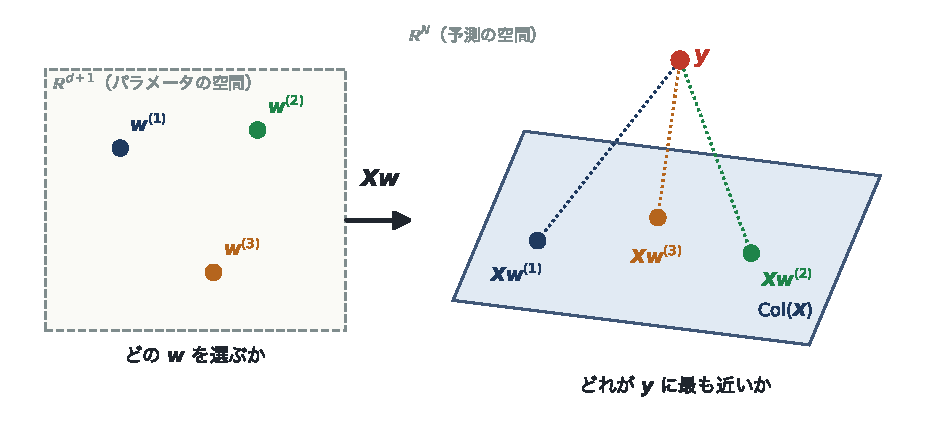
\includegraphics[width=\linewidth]{figures/ch4_rewrite}
  \caption{式\eqref{eq:ch4-rewrite}の読み替え。左はパラメータの空間、右は予測の空間であり、
  $\bm{X}$ を掛ける操作が両者を結んでいる。
  $\bm{w}^{(1)}, \bm{w}^{(2)}, \bm{w}^{(3)}$ はパラメータの選び方の例であり、
  それぞれが右の $\mathrm{Col}(\bm{X})$ 上の1点に対応する。
  パラメータをどう選ぶかという問いが、$\mathrm{Col}(\bm{X})$ 上のどの点が $\bm{y}$ に近いかという
  距離の問いに置き換わる。}
  \label{fig:ch4-rewrite}
\end{figure}

\subsubsection{直交性の原理}

幾何学的な直感を述べよう。
平面の外にある点から平面へ最短距離で行くには、\textbf{真下に垂直に降りればよい}。
斜めに降りれば遠回りになる。これを一般の部分空間に対して述べたものが次の定理である。

\begin{itembox}[l]{定理：直交性の原理}
$\bm{v}^* \in \mathrm{Col}(\bm{X})$ が
$\|\bm{y} - \bm{v}\|$ を $\bm{v} \in \mathrm{Col}(\bm{X})$ の範囲で最小にするための
必要十分条件は、誤差 $\bm{y} - \bm{v}^*$ が
列空間のすべてのベクトルと直交することである：
\begin{equation}
  \bm{u}^\top (\bm{y} - \bm{v}^*) = 0
  \qquad \text{（すべての } \bm{u} \in \mathrm{Col}(\bm{X}) \text{ に対して）}
  \label{eq:ch4-orth}
\end{equation}
このとき $\bm{v}^*$ を $\bm{y}$ の $\mathrm{Col}(\bm{X})$ への\textbf{正射影}と呼ぶ。
\end{itembox}

\subsubsection{証明：三平方の定理が効く}

\paragraph{十分性}
$\bm{y} - \bm{v}^*$ が列空間と直交していると仮定する。
$\bm{v} \in \mathrm{Col}(\bm{X})$ を任意にとる。
列空間は部分空間なので（第3.5.2項）、差 $\bm{v}^* - \bm{v}$ もまた列空間に属する。
したがって仮定より
\begin{equation*}
  (\bm{v}^* - \bm{v})^\top (\bm{y} - \bm{v}^*) = 0
\end{equation*}
である。ここで誤差を2つに分ける。
\begin{equation*}
  \bm{y} - \bm{v} = (\bm{y} - \bm{v}^*) + (\bm{v}^* - \bm{v})
\end{equation*}
この2つの項は直交しているので、第2回で示した三平方の定理
（$\bm{a} \perp \bm{b}$ のとき $\|\bm{a}+\bm{b}\|^2 = \|\bm{a}\|^2 + \|\bm{b}\|^2$）
が使えて
\begin{equation}
  \|\bm{y} - \bm{v}\|^2
  = \|\bm{y} - \bm{v}^*\|^2 + \|\bm{v}^* - \bm{v}\|^2
  \;\geq\; \|\bm{y} - \bm{v}^*\|^2
  \label{eq:ch4-pythagoras}
\end{equation}
を得る。

最後の不等号は、第2項 $\|\bm{v}^* - \bm{v}\|^2$ が\textbf{つねに $0$ 以上}であることから従う
（ノルムの非負性、第2.2.2項）。
右辺の第1項 $\|\bm{y} - \bm{v}^*\|^2$ は $\bm{v}$ に依存しない定数なので、
$\bm{v}$ をどう選んでも $\|\bm{y} - \bm{v}\|^2$ はこの定数より小さくなれない。

等号が成り立つのは第2項が $0$ になるとき、
すなわち $\|\bm{v}^* - \bm{v}\| = 0$、言い換えれば $\bm{v} = \bm{v}^*$ のときだけである
（ノルムが $0$ になるのは零ベクトルのときに限る、という非負性の後半を使った）。
よって $\bm{v}^*$ が唯一の最小点である。

\paragraph{必要性}
示したい主張を記号で置く。
\begin{align*}
  P &: \text{誤差 $\bm{y} - \bm{v}^*$ が $\mathrm{Col}(\bm{X})$ のすべてのベクトルと直交する} \\
  Q &: \text{$\bm{v}^*$ が $\|\bm{y} - \bm{v}\|$ を最小にする}
\end{align*}
必要性とは $Q \Rightarrow P$ のことである。
これを直接示すのは難しいので、\textbf{対偶} $\lnot P \Rightarrow \lnot Q$、すなわち
\begin{center}
「直交しないベクトルが一つでもあれば、$\bm{v}^*$ より近い点が作れる」
\end{center}
を示す。対偶が真であれば元の主張も真である。

\medskip
そこで、ある $\bm{u} \in \mathrm{Col}(\bm{X})$ に対して
\begin{equation*}
  \bm{u}^\top(\bm{y} - \bm{v}^*) = c \neq 0
\end{equation*}
であったとする（$\lnot P$ の仮定）。
このとき $\bm{u} \neq \bm{0}$ である。$\bm{u} = \bm{0}$ なら内積は $0$ になり、$c \neq 0$ に反するからである。

列空間は部分空間なので、任意の実数 $t$ に対して
$\bm{v}_t = \bm{v}^* + t\bm{u}$ もまた $\mathrm{Col}(\bm{X})$ に属する。
$\bm{u}$ の方向に $\bm{v}^*$ をずらした点である。
この点での誤差を、第2回で示した展開
$\|\bm{a}-\bm{b}\|^2 = \|\bm{a}\|^2 - 2\bm{a}^\top\bm{b} + \|\bm{b}\|^2$ を使って計算すると
\begin{align}
  \|\bm{y} - \bm{v}_t\|^2
    &= \|(\bm{y} - \bm{v}^*) - t\bm{u}\|^2 \notag \\
    &= \|\bm{y} - \bm{v}^*\|^2 - 2t\,\bm{u}^\top(\bm{y} - \bm{v}^*) + t^2\|\bm{u}\|^2 \notag \\
    &= \|\bm{y} - \bm{v}^*\|^2 + g(t),
      \qquad g(t) = t^2\|\bm{u}\|^2 - 2ct
  \label{eq:ch4-necessity}
\end{align}
となる。$\bm{v}^*$ より誤差を小さくできるかは、\textbf{$g(t)$ を負にできるか}だけで決まる。

$g$ は $t$ の下に凸な2次関数であり、$g(0) = 0$ である。
$g'(t) = 2t\|\bm{u}\|^2 - 2c = 0$ より $t = c/\|\bm{u}\|^2$ で最小になる。
この値を代入すると
\begin{equation}
  g\!\left( \frac{c}{\|\bm{u}\|^2} \right)
   = \frac{c^2}{\|\bm{u}\|^2} - \frac{2c^2}{\|\bm{u}\|^2}
   = -\frac{c^2}{\|\bm{u}\|^2} \;<\; 0
  \label{eq:ch4-gmin}
\end{equation}
である。$c \neq 0$ より分子は正、$\bm{u} \neq \bm{0}$ より分母は正だからである。
したがって、この $t$ に対して
\begin{equation*}
  \|\bm{y} - \bm{v}_t\|^2
   = \|\bm{y} - \bm{v}^*\|^2 - \frac{c^2}{\|\bm{u}\|^2}
   \;<\; \|\bm{y} - \bm{v}^*\|^2
\end{equation*}
となる。$\bm{v}^*$ より $\bm{y}$ に近い点が $\mathrm{Col}(\bm{X})$ の中に実際に見つかったので、
$\bm{v}^*$ は最小点ではない。すなわち $\lnot Q$ である。

\medskip
これで $\lnot P \Rightarrow \lnot Q$ が示された。対偶をとると
\begin{center}
$Q \Rightarrow P$：\quad $\bm{v}^*$ が最小点ならば、誤差は $\mathrm{Col}(\bm{X})$ のすべてのベクトルと直交する
\end{center}
となり、これが示したかった必要性である。\hfill $\blacksquare$

\medskip
\noindent
なお、最適な $t = c/\|\bm{u}\|^2$ には意味がある。これは
\begin{equation*}
  t\bm{u} = \frac{\bm{u}^\top(\bm{y} - \bm{v}^*)}{\|\bm{u}\|^2}\,\bm{u}
\end{equation*}
と書けるので、\textbf{誤差 $\bm{y}-\bm{v}^*$ を $\bm{u}$ の方向へ正射影したベクトル}そのものである
（第2.4.3項）。
直交していない分だけ $\bm{u}$ 方向に動けば、その分だけ誤差が縮む。
ここでも正射影が顔を出している。

\begin{figure}[H]
  \centering
  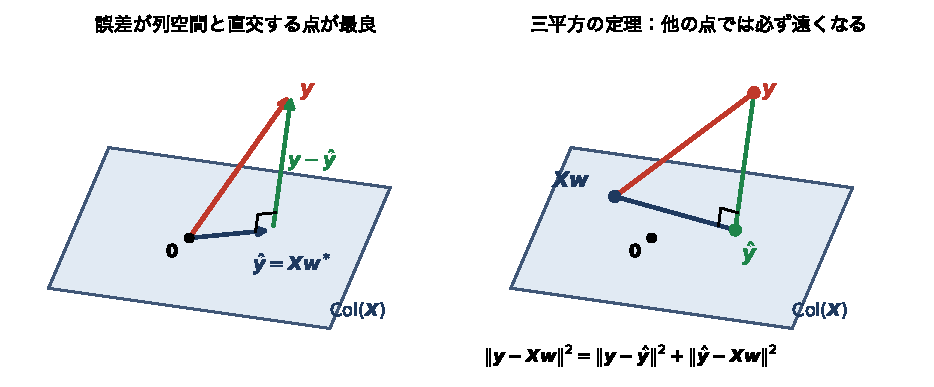
\includegraphics[width=\linewidth]{figures/ch4_projection}
  \caption{最小二乗法の幾何学。左：誤差 $\bm{y}-\hat{\bm{y}}$ が列空間と直交する点が最良の予測である。
  右：列空間上の他の点 $\bm{X}\bm{w}$ をとると、三平方の定理により
  $\|\bm{y}-\bm{X}\bm{w}\|^2 = \|\bm{y}-\hat{\bm{y}}\|^2 + \|\hat{\bm{y}}-\bm{X}\bm{w}\|^2$
  となり、必ず遠くなる。}
  \label{fig:ls-projection}
\end{figure}

\subsubsection{直交条件を行列の式に直す}

あとは式\eqref{eq:ch4-orth}を計算できる形に書き直すだけである。

列空間のすべてのベクトルと直交することは、
\textbf{$\bm{X}$ のすべての列と直交すること}と同じである。
なぜなら列空間の任意の元は列の線形結合であり、
各列と直交していればその線形結合とも直交するからである。

$\bm{X}$ の列を $\bm{c}_0, \ldots, \bm{c}_d$、$\bm{v}^* = \bm{X}\bm{w}$ と書くと、条件は
\begin{equation*}
  \bm{c}_j^\top (\bm{y} - \bm{X}\bm{w}) = 0 \qquad (j = 0, 1, \ldots, d)
\end{equation*}
である。この $d+1$ 本の式は、第3.2.1項の\textbf{見方1}（行との内積）を使えば
一つの行列の式にまとまる。
$\bm{X}^\top$ の第 $j$ 行は $\bm{X}$ の第 $j$ 列 $\bm{c}_j$ にほかならないので、
\begin{equation}
  \bm{X}^\top (\bm{y} - \bm{X}\bm{w}) = \bm{0}
  \label{eq:ch4-orth-matrix}
\end{equation}
と書ける。$\bm{X}^\top$ を左から掛けるという操作が、
「すべての列との内積を一度に取る」という操作に対応しているわけである。

これを整理すれば目的の式が得られる。

\begin{itembox}[l]{定義：正規方程式}
経験損失 $\frac{1}{N}\|\bm{y} - \bm{X}\bm{w}\|^2$ を最小にする $\bm{w}$ は、
\begin{equation}
  \bm{X}^\top \bm{X} \bm{w} = \bm{X}^\top \bm{y}
  \label{eq:normal-equation}
\end{equation}
を満たす。この連立一次方程式を\textbf{正規方程式}（normal equation）と呼ぶ。
\end{itembox}

$\bm{X}^\top\bm{X}$ は $(d+1) \times (d+1)$ の正方行列、
$\bm{X}^\top\bm{y}$ は $d+1$ 次元のベクトルである。
元の問題は $N$ 件（数万件かもしれない）のデータに関する最小化問題だったが、
それが $d+1$ 本の連立一次方程式に縮んだ。
これが正規方程式のありがたみである。

なお「正規」は normal の訳で、ここでは\textbf{直交}（normal＝法線）の意味である。
誤差が列空間の法線方向を向いている、という条件から出てきた式だからこう呼ばれる。


\subsection{微分による導出}

同じ式を、今度は解析的に導く。
こちらは幾何学的な洞察を必要としない代わりに、機械的に計算できる。

\subsubsection{1変数の場合の復習}

まず1変数で感覚を取り戻しておこう。$a > 0$ として
\begin{equation*}
  f(w) = a w^2 - 2bw + c
\end{equation*}
という下に凸な2次関数を考える。最小点は微分して $0$ とおけば求まる：
\begin{equation*}
  f'(w) = 2aw - 2b = 0 \quad \Longrightarrow \quad w = \frac{b}{a}
\end{equation*}

これから見るように、$L_D(\bm{w})$ はこの式の多変数版であり、
$a$ にあたるのが $\bm{X}^\top\bm{X}$、$b$ にあたるのが $\bm{X}^\top\bm{y}$ である。

\subsubsection{勾配}

多変数の場合、「微分して $0$」は各変数についての偏微分をすべて $0$ にすることである。
これをベクトルにまとめたものを勾配と呼ぶ。

\begin{itembox}[l]{定義：偏微分と勾配}
$f : \mathbb{R}^p \to \mathbb{R}$ に対して、
第 $i$ 変数だけを動かし他を固定して微分したものを
\textbf{偏微分}（partial derivative）と呼び $\dfrac{\partial f}{\partial w_i}$ と書く。
これらを縦に並べたベクトル
\begin{equation}
  \nabla f(\bm{w}) =
  \left( \frac{\partial f}{\partial w_1},\;
         \frac{\partial f}{\partial w_2},\; \ldots,\;
         \frac{\partial f}{\partial w_p} \right)^\top \in \mathbb{R}^p
\end{equation}
を $f$ の\textbf{勾配}（gradient）と呼ぶ。記号 $\nabla$ は「ナブラ」と読む。
\end{itembox}

勾配には明確な幾何学的意味がある。
$\nabla f(\bm{w})$ は、その点で\textbf{$f$ が最も急に増える向き}を指し、
その大きさ $\|\nabla f(\bm{w})\|$ は増え方の急さを表す。
したがって $-\nabla f(\bm{w})$ は最も急に減る向きであり、
これが第5回で学ぶ\textbf{勾配降下法}の原理になる。

図\ref{fig:gradient-concept}で具体例を見ておこう。
$f(w_1, w_2) = w_1^2 + 2w_2^2$ の偏微分は
$\partial f/\partial w_1 = 2w_1$、$\partial f/\partial w_2 = 4w_2$ であり、
左図のように、それぞれ曲面を $w_1$ 軸・$w_2$ 軸に平行に切った断面曲線の傾きである。
点 $\bm{w} = (1, 0.5)^\top$ ではどちらも $2$ なので $\nabla f(\bm{w}) = (2, 2)^\top$ となる。
右図はこれを等高線の上に描いたもので、2つの偏微分がそのまま矢印の成分になっている。
勾配はつねに等高線と直交し、等高線が密な（＝急な）場所ほど長い。
$w_2$ 方向の係数が大きいため等高線は横長の楕円になり、
同じ距離だけ動いても $w_2$ 方向の方が $f$ は速く増える。

\begin{figure}[H]
  \centering
  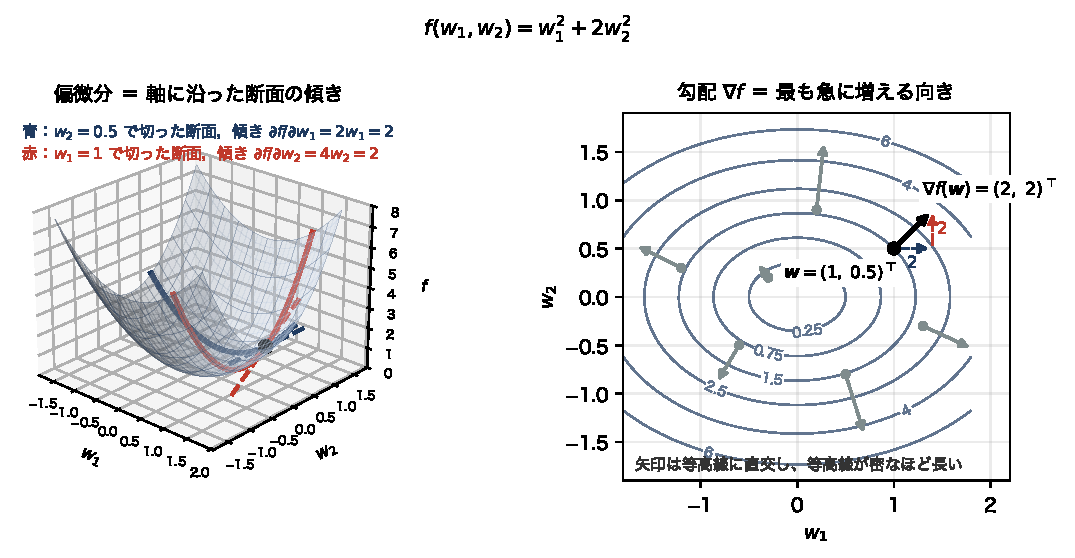
\includegraphics[width=\linewidth]{figures/ch4_gradient_concept}
  \caption{$f(w_1, w_2) = w_1^2 + 2w_2^2$ における偏微分と勾配。
  左：偏微分は曲面を各軸に平行に切った断面（青・赤の曲線）の傾き（破線）である。
  右：同じ関数の等高線と勾配ベクトル。点 $(1, 0.5)^\top$ での勾配 $(2, 2)^\top$ は
  2つの偏微分を成分に持ち、灰色の矢印も含めすべて等高線に直交する。}
  \label{fig:gradient-concept}
\end{figure}

関数が滑らかで下に凸なとき、最小点では $\nabla f(\bm{w}) = \bm{0}$ となる。
どの向きに動いても増えも減りもしない、という状態である。

\subsubsection{必要な2つの公式}

$L_D$ を微分するために、行列・ベクトルの微分公式を2つだけ用意する。

\begin{itembox}[l]{公式：ベクトルによる微分}
$\bm{a} \in \mathbb{R}^p$ を定ベクトル、$\bm{A} \in \mathbb{R}^{p \times p}$ を\textbf{対称}な定行列とする。
\begin{align}
  \nabla_{\bm{w}} \left( \bm{a}^\top \bm{w} \right) &= \bm{a} \label{eq:grad-linear} \\
  \nabla_{\bm{w}} \left( \bm{w}^\top \bm{A} \bm{w} \right) &= 2\bm{A}\bm{w} \label{eq:grad-quad}
\end{align}
\end{itembox}

\paragraph{1次の項の公式の証明}
$\bm{a}^\top\bm{w} = \sum_{j} a_j w_j$ であるから、$w_i$ について偏微分すると
$w_i$ を含む項は $a_i w_i$ だけで、
\begin{equation*}
  \frac{\partial}{\partial w_i} \sum_{j} a_j w_j = a_i
\end{equation*}
これを並べると $\bm{a}$ になる。\hfill $\blacksquare$

\paragraph{2次の項の公式の証明}
$\bm{w}^\top\bm{A}\bm{w} = \sum_{j}\sum_{k} a_{jk} w_j w_k$ である。
$w_i$ を含むのは、$j = i$ の項、$k = i$ の項、および $j = k = i$ の項である。
積の微分に注意して
\begin{align*}
  \frac{\partial}{\partial w_i} \sum_{j}\sum_{k} a_{jk} w_j w_k
    &= \sum_{k} a_{ik} w_k + \sum_{j} a_{ji} w_j \\
    &= (\bm{A}\bm{w})_i + (\bm{A}^\top \bm{w})_i
\end{align*}
$\bm{A}$ が対称なら $\bm{A}^\top = \bm{A}$ なので、これは $2(\bm{A}\bm{w})_i$ に等しい。
並べれば $2\bm{A}\bm{w}$ である。\hfill $\blacksquare$

対称性の仮定は本質的である。我々が扱う $\bm{A} = \bm{X}^\top\bm{X}$ は
つねに対称なので（第4.5.1項）、この公式がそのまま使える。

\subsubsection{経験損失を展開して微分する}

$L_D(\bm{w}) = \frac{1}{N}\|\bm{y} - \bm{X}\bm{w}\|^2$（式\eqref{eq:ch4-setup}）を展開する。
ここで $N$ はデータ件数である。
係数 $\frac{1}{N}$ を毎回書くのは煩わしいので、両辺を $N$ 倍した $N \cdot L_D(\bm{w})$ を扱う。
定数倍しても最小点は変わらないので（第4.1.1項）、勾配を $\bm{0}$ とおく議論には影響しない。
$\|\bm{z}\|^2 = \bm{z}^\top\bm{z}$ を使うと
\begin{align}
  N \cdot L_D(\bm{w})
    &= (\bm{y} - \bm{X}\bm{w})^\top (\bm{y} - \bm{X}\bm{w}) \notag \\
    &= \bm{y}^\top\bm{y}
       - \bm{y}^\top\bm{X}\bm{w}
       - (\bm{X}\bm{w})^\top\bm{y}
       + (\bm{X}\bm{w})^\top\bm{X}\bm{w} \notag \\
    &= \bm{y}^\top\bm{y}
       - 2\,(\bm{X}^\top\bm{y})^\top \bm{w}
       + \bm{w}^\top (\bm{X}^\top\bm{X}) \bm{w}
  \label{eq:ch4-expand}
\end{align}
2行目から3行目では、$(\bm{X}\bm{w})^\top\bm{y} = \bm{w}^\top\bm{X}^\top\bm{y}$ が
スカラーであり、スカラーは転置しても変わらないことから
$\bm{y}^\top\bm{X}\bm{w} = \bm{w}^\top\bm{X}^\top\bm{y} = (\bm{X}^\top\bm{y})^\top\bm{w}$
となることを用いた。
また $(\bm{X}\bm{w})^\top\bm{X}\bm{w} = \bm{w}^\top\bm{X}^\top\bm{X}\bm{w}$ である
（転置すると積の順序が逆になる、第3.2.4項）。

式\eqref{eq:ch4-expand}は、1変数のときの $aw^2 - 2bw + c$ と
まったく同じ形をしている。あとは公式を当てはめるだけである。
第1項は $\bm{w}$ を含まないので消え、第2項に式\eqref{eq:grad-linear}、
第3項に式\eqref{eq:grad-quad}を使って
\begin{equation}
  \nabla_{\bm{w}} \bigl( N \cdot L_D(\bm{w}) \bigr)
  = -2\,\bm{X}^\top\bm{y} + 2\,\bm{X}^\top\bm{X}\bm{w}
\end{equation}
を得る。これを $\bm{0}$ とおくと
\begin{equation*}
  \bm{X}^\top\bm{X}\bm{w} = \bm{X}^\top\bm{y}
\end{equation*}
となり、幾何学から導いた式\eqref{eq:normal-equation}と\textbf{完全に一致する}。

\begin{figure}[H]
  \centering
  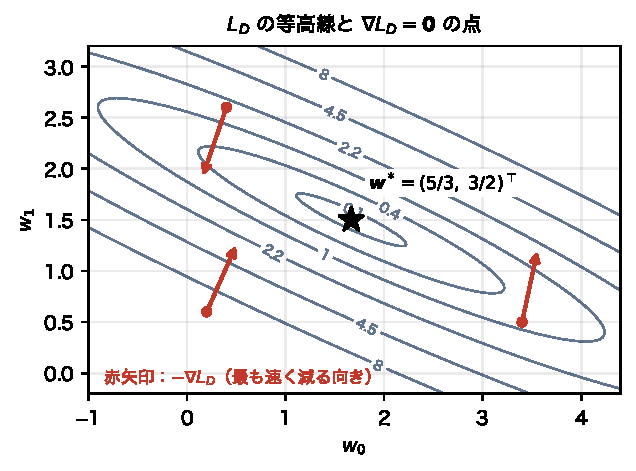
\includegraphics[width=0.62\linewidth]{figures/ch4_gradient}
  \caption{後述の数値例（$D = \{(1,3), (2,5), (3,6)\}$）における経験損失の等高線。
  赤い矢印は $-\nabla L_D$、すなわち損失が最も速く減る向きである。
  中央の $\bm{w}^*$ では勾配が $\bm{0}$ になり、どの向きに動いても損失は増える。}
  \label{fig:ls-gradient}
\end{figure}

\subsubsection{停留点が最小値である理由}

$\nabla L_D = \bm{0}$ は、厳密には「接平面が水平な点」（\textbf{停留点}）の条件であって、
それだけでは最小・最大・鞍点のどれかは分からない。
ここで最小だと言い切れるのは、$L_D$ が下に凸だからである。

1変数の $f(w) = aw^2 - 2bw + c$ では、2階微分 $f''(w) = 2a$ の符号がすべてを決めていた。
$a > 0$ なら下に凸で停留点はただ一つの最小点、
$a = 0$ なら曲がっておらず（直線）停留点は最小点とは限らず、
$a < 0$ なら上に凸で停留点は最大点である。

多変数で $f''$ の役割を果たすのが、2階偏微分を並べた次の行列である。

\begin{itembox}[l]{定義：ヘッセ行列}
$f : \mathbb{R}^p \to \mathbb{R}$ が2回微分可能なとき、
すべての2階偏微分を $p \times p$ に並べた行列
\begin{equation}
  \nabla^2 f(\bm{w}) =
  \begin{pmatrix}
    \dfrac{\partial^2 f}{\partial w_1^2} &
    \dfrac{\partial^2 f}{\partial w_1 \partial w_2} & \cdots &
    \dfrac{\partial^2 f}{\partial w_1 \partial w_p} \\[2ex]
    \dfrac{\partial^2 f}{\partial w_2 \partial w_1} &
    \dfrac{\partial^2 f}{\partial w_2^2} & \cdots &
    \dfrac{\partial^2 f}{\partial w_2 \partial w_p} \\
    \vdots & \vdots & \ddots & \vdots \\[1ex]
    \dfrac{\partial^2 f}{\partial w_p \partial w_1} &
    \dfrac{\partial^2 f}{\partial w_p \partial w_2} & \cdots &
    \dfrac{\partial^2 f}{\partial w_p^2}
  \end{pmatrix}
  \in \mathbb{R}^{p \times p}
\end{equation}
を $f$ の\textbf{ヘッセ行列}（Hessian matrix）と呼ぶ。
$(i, j)$ 成分は $\partial^2 f / \partial w_i \partial w_j$、
すなわち「$w_j$ で偏微分してから $w_i$ で偏微分したもの」である。
$f$ が滑らかなら偏微分の順序は交換できる
（$\partial^2 f / \partial w_i \partial w_j = \partial^2 f / \partial w_j \partial w_i$）ので、
ヘッセ行列は\textbf{対称行列}である。
勾配 $\nabla f$ が「1階微分を並べたベクトル」であったのに対し、
ヘッセ行列は「2階微分を並べた行列」であり、$\nabla^2$ はその意味の記号である。
\end{itembox}

$p = 1$ のときヘッセ行列は $1 \times 1$ 行列 $(f'')$ にほかならない。
ただし多変数では「曲がり方」が方向ごとに異なりうる。
点 $\bm{w}$ から向き $\bm{v} \in \mathbb{R}^p$ に沿って進んだときの $f$ の曲がり方、
すなわち $g(t) = f(\bm{w} + t\bm{v})$ の2階微分は
\begin{equation}
  g''(0) = \bm{v}^\top \bigl( \nabla^2 f(\bm{w}) \bigr) \bm{v}
  \label{eq:ch4-directional-curvature}
\end{equation}
で与えられる。
つまり「ヘッセ行列に $\bm{v}$ を挟んだもの」は\textbf{向き $\bm{v}$ での2階微分}である。
これが、第2.3.2項で定義した正定値・半正定値が
ここで登場する理由である。

\begin{itembox}[l]{定義（再掲）：正定値と半正定値}
対称行列 $\bm{A} \in \mathbb{R}^{p \times p}$ について
\begin{align*}
  \text{正定値（positive definite）：} \quad
    & \bm{v}^\top \bm{A}\bm{v} > 0 \quad (\text{すべての } \bm{v} \neq \bm{0}) \\
  \text{半正定値（positive semi-definite）：} \quad
    & \bm{v}^\top \bm{A}\bm{v} \geq 0 \quad (\text{すべての } \bm{v})
\end{align*}
等号 $\bm{v}^\top \bm{A}\bm{v} = 0$ を $\bm{v} \neq \bm{0}$ に対して許すかどうかが両者を分ける。
\end{itembox}

\paragraph{直感的な意味}
ヘッセ行列に限らず、正定値・半正定値は次の3通りに捉えるとよい。
図\ref{fig:definiteness}に、正定値な $\bm{A}$ と半正定値止まりの $\bm{B}$ を並べて3つの見方を示した。

\textbf{「正の数」の行列版。}
1変数で $a > 0$ は「$a v^2 > 0$ がすべての $v \neq 0$ で成り立つ」と言い換えられる。
$\bm{v}^\top \bm{A}\bm{v} = \sum_{i}\sum_{j} a_{ij} v_i v_j$ は $a v^2$ の多変数版（2次形式）であり、
これがつねに正になる $\bm{A}$ が正定値、つねに非負になる $\bm{A}$ が半正定値である。
つまり正定値は「正の数」、半正定値は「非負の数」の行列への拡張であり、
$a > 0$ と $a \geq 0$ の違いがそのまま両者の違いにあたる。
例えば
\begin{equation*}
  \bm{A} = \begin{pmatrix} 1 & 0 \\ 0 & 2 \end{pmatrix}
  \;\Longrightarrow\; \bm{v}^\top \bm{A}\bm{v} = v_1^2 + 2 v_2^2, \qquad
  \bm{B} = \begin{pmatrix} 1 & 0 \\ 0 & 0 \end{pmatrix}
  \;\Longrightarrow\; \bm{v}^\top \bm{B}\bm{v} = v_1^2
\end{equation*}
で、$\bm{A}$ は正定値（図\ref{fig:gradient-concept}左のお椀の形がまさに $\bm{v}^\top \bm{A}\bm{v}$ のグラフである）、
$\bm{B}$ は半正定値だが正定値ではない。
$\bm{B}$ では $\bm{v} = (0, 1)^\top$ のように $v_2$ 方向へ動いても値が変わらず、
グラフはお椀ではなく、$v_2$ 方向に平らな\textbf{樋（とい）の形}になる。
この「値が変わらない向き」が、第2.3.2項で述べた「つぶれた方向」である。

\textbf{向きをほぼ保つ変換。}
$\bm{v}^\top \bm{A}\bm{v} = \bm{v}^\top (\bm{A}\bm{v})$ は、
$\bm{v}$ と、それを $\bm{A}$ で変換した $\bm{A}\bm{v}$ との内積である。
第2回の内積の意味から、これが正であることは
$\bm{v}$ と $\bm{A}\bm{v}$ のなす角が $90^\circ$ 未満であることを意味する。
すなわち正定値な $\bm{A}$ は、どのベクトルも $90^\circ$ 以上は回さない
（おおまかに向きを保つ）変換である。
半正定値では、ちょうど $90^\circ$ 回す場合や、$\bm{A}\bm{v} = \bm{0}$ につぶす場合までが許される。

\textbf{固有値で見る。}
対称行列 $\bm{A}$ については、正定値であることは固有値がすべて正であること、
半正定値であることは固有値がすべて非負であることと同値である（第3.7節）。
固有値 $0$ に対応する固有ベクトルの向きが、上で述べた「つぶれた方向」にほかならない。
上の例では $\bm{A}$ の固有値は $1, 2$、$\bm{B}$ の固有値は $1, 0$ である。

\begin{figure}[H]
  \centering
  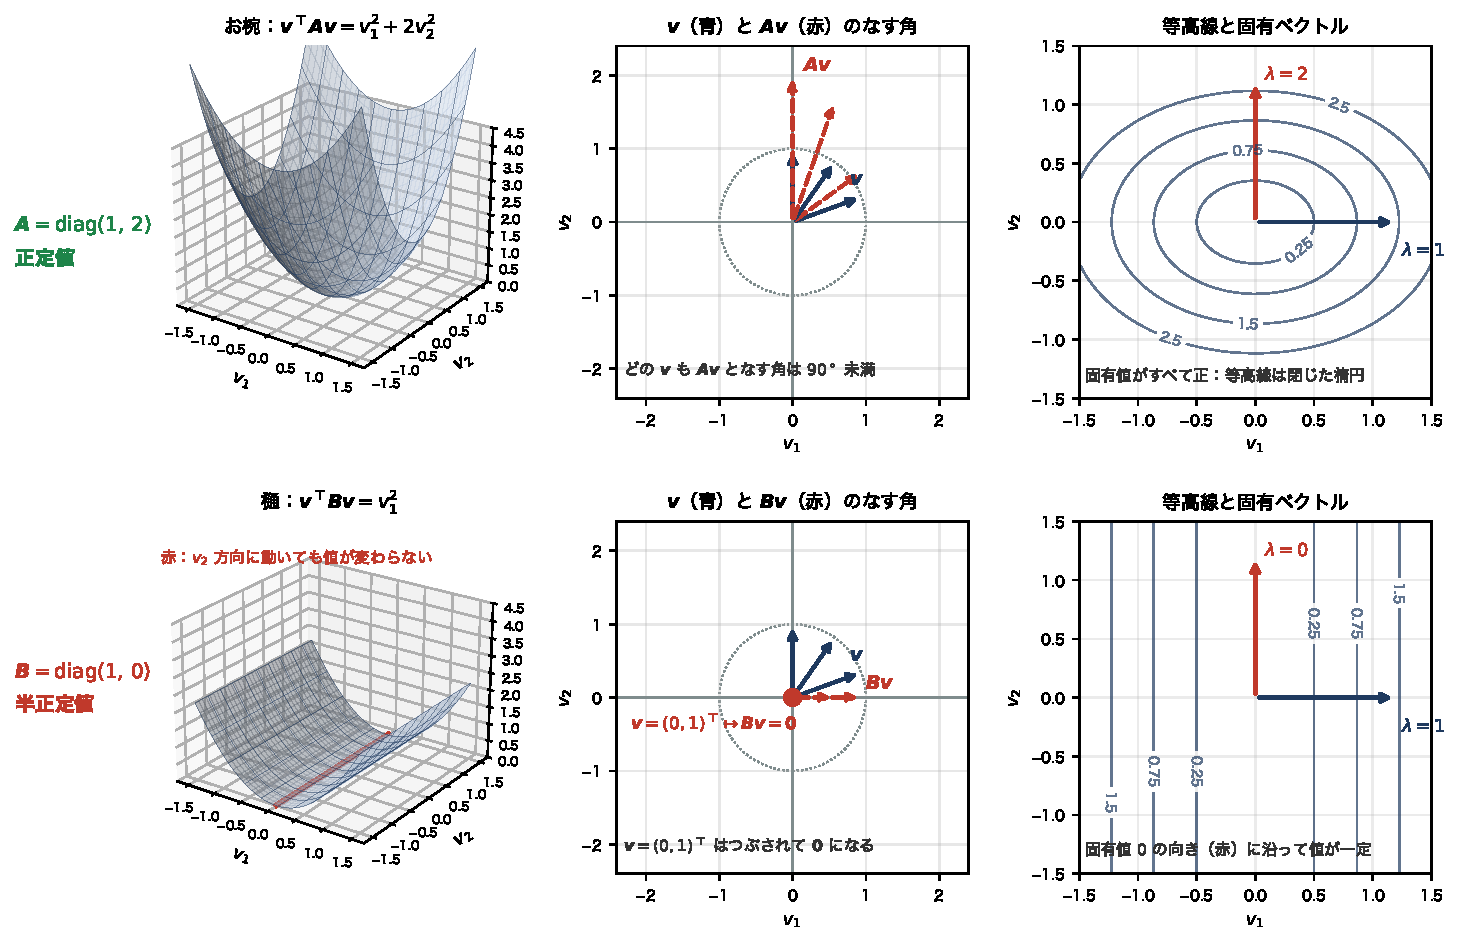
\includegraphics[width=\linewidth]{figures/ch4_definiteness}
  \caption{正定値（上段：$\bm{A} = \mathrm{diag}(1,2)$）と半正定値（下段：$\bm{B} = \mathrm{diag}(1,0)$）の3つの見方。
  左：2次形式 $\bm{v}^\top\bm{A}\bm{v}$ のグラフはお椀、$\bm{v}^\top\bm{B}\bm{v}$ は $v_2$ 方向に平らな樋になる。
  中：$\bm{v}$（青）と $\bm{A}\bm{v}$（赤）のなす角はつねに $90^\circ$ 未満だが、
  $\bm{B}$ は $\bm{v} = (0,1)^\top$ を $\bm{0}$ につぶす。
  右：$\bm{A}$ の等高線は閉じた楕円で固有値はすべて正、
  $\bm{B}$ は固有値 $0$ の固有ベクトルの向きに沿って値が一定で、等高線が閉じない。}
  \label{fig:definiteness}
\end{figure}

\paragraph{ヘッセ行列の場合}
$\bm{A}$ がヘッセ行列のとき、式\eqref{eq:ch4-directional-curvature}より
$\bm{v}^\top \bm{A}\bm{v}$ は向き $\bm{v}$ での曲がり方なので、上の直感は次のように翻訳される。
\begin{itemize}
  \item \textbf{正定値}：どの向きに進んでも $f$ は上に曲がる（お椀の形）。
    停留点は\textbf{ただ一つの}最小点である。
  \item \textbf{半正定値}：どの向きにも下には曲がらないが、
    $\bm{v}^\top \bm{A}\bm{v} = 0$ となる「平らな向き」があってよい（樋の形）。
    停留点は最小点ではあるが、平らな向きに沿って最小点が\textbf{無数に}連なりうる。
\end{itemize}

$L_D$ の場合を見よう。式\eqref{eq:ch4-expand}をもう一度微分すると
\begin{equation}
  \nabla^2 L_D(\bm{w}) = \frac{2}{N}\,\bm{X}^\top\bm{X}
\end{equation}
であり、これは $\bm{w}$ によらない定行列である。
そして任意の $\bm{v} \in \mathbb{R}^{d+1}$ に対して
\begin{equation}
  \bm{v}^\top (\bm{X}^\top\bm{X}) \bm{v} = (\bm{X}\bm{v})^\top (\bm{X}\bm{v}) = \|\bm{X}\bm{v}\|^2 \geq 0
  \label{eq:ch4-psd}
\end{equation}
であるから、$\bm{X}^\top\bm{X}$ は少なくとも\textbf{半正定値}である。
よって $L_D$ はどの向きにも下に曲がらず（下に凸）、停留点は\textbf{大域的な最小点}である。
これで「勾配が $\bm{0}$ の点が最小点だ」と言い切ってよい理由が確かめられた。

さらに式\eqref{eq:ch4-psd}を見ると、
等号 $\|\bm{X}\bm{v}\|^2 = 0$ が成り立つのは $\bm{X}\bm{v} = \bm{0}$ のときだけである。
したがって $\bm{X}^\top\bm{X}$ が正定値か半正定値にとどまるかは、
$\bm{X}\bm{v} = \bm{0}$ となる $\bm{v} \neq \bm{0}$ が存在するかどうか、
すなわち $\bm{X}$ がフルランクかどうかで決まる。
\begin{itemize}
  \item $\bm{X}$ がフルランク：$\bm{X}^\top\bm{X}$ は\textbf{正定値}。
    最小点は一意に定まる（第4.5.3項）。
  \item $\bm{X}$ がランク落ち：$\bm{X}^\top\bm{X}$ は\textbf{半正定値だが正定値ではない}。
    $\bm{X}\bm{v} = \bm{0}$ の向きには $L_D$ が平らで、
    最小点がその向きに沿って無数に並ぶ（第3回の図\ref{fig:flat-valley}、第4.7節）。
\end{itemize}

式\eqref{eq:ch4-psd}は本章で何度も使う。覚えておく価値がある。
「$\bm{X}^\top\bm{X}$ に $\bm{v}$ を挟んだものは $\bm{X}\bm{v}$ の長さの二乗」という事実である。
凸関数の一般論は第5回で扱う。


\subsection{2つの導出の対応}

同じ式に2通りで到達した。両者の関係を整理しておく。

\begin{center}
\begin{tabular}{l|p{4.6cm}|p{4.6cm}}
\hline
 & 幾何学（射影） & 微分 \\
\hline\hline
出発点 & 列空間の中で $\bm{y}$ に最も近い点を探す & $L_D(\bm{w})$ を $\bm{w}$ の関数とみて微分する \\
\hline
鍵となる事実 & 誤差が列空間と直交する & 勾配が $\bm{0}$ になる \\
\hline
使う道具 & 三平方の定理、内積 & 偏微分、行列の展開 \\
\hline
分かること & \textbf{なぜ}その式なのか。$\hat{\bm{y}}$ が射影であること & 損失を変えても\textbf{同じ手順}で解けること \\
\hline
\end{tabular}
\end{center}

この2つは実は同じことを言っている。
式\eqref{eq:ch4-orth-matrix}の左辺 $\bm{X}^\top(\bm{y} - \bm{X}\bm{w})$ は、
符号と定数倍を除いてそのまま勾配 $\nabla L_D$ である。
つまり\textbf{「勾配が $\bm{0}$」と「誤差が列空間と直交」は同じ条件}なのである。

どちらを使うべきか。目的によって使い分けるのがよい。
たとえば第6回で扱うリッジ回帰では、損失に $\lambda\|\bm{w}\|^2$ という項が加わる。
このとき微分による導出は、公式\eqref{eq:grad-quad}をもう一度使うだけで済む。
一方、正則化が解をどう変えるかを図で理解したいときには、
幾何学的な描像のほうが役に立つ。


\subsection{正規方程式を解く}

正規方程式 $\bm{X}^\top\bm{X}\bm{w} = \bm{X}^\top\bm{y}$ が得られた。
これを $\bm{w}$ について解きたい。

\subsubsection{\texorpdfstring{$\bm{X}^\top\bm{X}$}{X\^{}TX} の性質}

まず相手を知っておく。$\bm{X} \in \mathbb{R}^{N \times (d+1)}$ に対して
$\bm{X}^\top\bm{X}$ は次の性質をもつ。

\begin{itemize}
  \item \textbf{正方行列}である。
    $(d+1) \times N$ と $N \times (d+1)$ の積なので $(d+1) \times (d+1)$ になる。
    データ件数 $N$ がいくら大きくてもサイズは変わらない。
  \item \textbf{対称}である。
    $(\bm{X}^\top\bm{X})^\top = \bm{X}^\top (\bm{X}^\top)^\top = \bm{X}^\top\bm{X}$。
  \item \textbf{半正定値}である。式\eqref{eq:ch4-psd}で示したとおり。
  \item 第 $(i,j)$ 成分は $\bm{c}_i^\top\bm{c}_j$、すなわち\textbf{列どうしの内積}である。
    対角成分は $\|\bm{c}_i\|^2$ になる。
\end{itemize}

最後の項目は見逃せない。$\bm{X}^\top\bm{X}$ は
\textbf{特徴どうしの関係をまとめた表}なのである。
第3.5.5項で見た多重共線性、すなわち特徴どうしが似ている状況は、
この行列の性質としてはっきり現れる。

\subsubsection{逆行列}

連立一次方程式 $\bm{A}\bm{w} = \bm{b}$ を解くとは、
1変数の $aw = b$ を $w = b/a$ と解くことの行列版である。
「$a$ で割る」にあたる操作を与えるのが逆行列である。

\begin{itembox}[l]{定義：逆行列}
正方行列 $\bm{A} \in \mathbb{R}^{n \times n}$ に対して
\begin{equation}
  \bm{A}\bm{B} = \bm{B}\bm{A} = \bm{I}_n
\end{equation}
を満たす $\bm{B}$ が存在するとき、$\bm{A}$ は\textbf{正則}（regular, invertible）であるといい、
$\bm{B}$ を $\bm{A}$ の\textbf{逆行列}（inverse matrix）と呼んで $\bm{A}^{-1}$ と書く。
逆行列は存在すればただ一つである。
\end{itembox}

一意性は次のように確かめられる。$\bm{B}, \bm{C}$ がともに逆行列だとすると
\begin{equation*}
  \bm{B} = \bm{B}\bm{I}_n = \bm{B}(\bm{A}\bm{C}) = (\bm{B}\bm{A})\bm{C} = \bm{I}_n\bm{C} = \bm{C}
\end{equation*}
となる。

$2\times2$ の場合は具体的に書ける。$\det\bm{A} = ad - bc \neq 0$ のとき
\begin{equation}
  \bm{A} = \begin{pmatrix} a & b \\ c & d \end{pmatrix}
  \quad \Longrightarrow \quad
  \bm{A}^{-1} = \frac{1}{ad - bc} \begin{pmatrix} d & -b \\ -c & a \end{pmatrix}
  \label{eq:inv2}
\end{equation}
逆に $\det\bm{A} = 0$、すなわち列が線形従属なときは逆行列が存在しない。
第3.7.2項で見たとおり、$\det\bm{A} = 0$ は「列がつぶれている」ことの印であった。
つぶれた変換は元に戻せない、と考えると納得しやすい。

\subsubsection{解が一意に定まる条件}

いつ $\bm{X}^\top\bm{X}$ は正則になるのか。答えは第3回のランクで決まる。

\begin{itembox}[l]{定理：正規方程式の一意可解性}
$\bm{X} \in \mathbb{R}^{N \times (d+1)}$ について、次の3つは同値である。
\begin{enumerate}
  \item $\bm{X}$ の列が線形独立である（$\mathrm{rank}(\bm{X}) = d+1$、フルランク）
  \item $\bm{X}^\top\bm{X}$ が正定値である
  \item $\bm{X}^\top\bm{X}$ が正則である
\end{enumerate}
このとき正規方程式の解は一意に定まり、
\begin{equation}
  \bm{w}^* = (\bm{X}^\top\bm{X})^{-1}\bm{X}^\top\bm{y}
  \label{eq:ls-solution}
\end{equation}
である。
\end{itembox}

\paragraph{証明の要点}
(1) $\Rightarrow$ (2)：$\bm{v} \neq \bm{0}$ とすると、列が線形独立なので $\bm{X}\bm{v} \neq \bm{0}$ である。
よって式\eqref{eq:ch4-psd}より $\bm{v}^\top\bm{X}^\top\bm{X}\bm{v} = \|\bm{X}\bm{v}\|^2 > 0$ となり、正定値。

(2) $\Rightarrow$ (3)：正定値なら固有値はすべて正なので $0$ を固有値にもたない。
第3.7.4項より、固有値 $0$ をもたないことはランク落ちしていないことと同値であり、正則である。

(3) $\Rightarrow$ (1)：対偶を示す。列が線形従属なら $\bm{X}\bm{v} = \bm{0}$ となる
$\bm{v} \neq \bm{0}$ が存在し（第3.5.5項）、このとき $\bm{X}^\top\bm{X}\bm{v} = \bm{0}$ となる。
正則な行列は $\bm{0}$ でないベクトルを $\bm{0}$ に写さないので、$\bm{X}^\top\bm{X}$ は正則でない。
\hfill $\blacksquare$

フルランクであるためには、少なくとも $N \geq d+1$ が必要である
（$\mathrm{rank}(\bm{X}) \leq \min(N, d+1)$ だから）。
\textbf{データ件数が特徴数より少なければ、この方法では解が定まらない}。
現代の機械学習ではこの状況がごく普通に起こる。
その場合の扱いが第4.7節の主題である。

\subsubsection{数値例}

第1回の演習問題で扱ったデータを使う。
$D = \{(1, 3),\; (2, 5),\; (3, 6)\}$ に、
バイアス項つきの直線 $h(x) = w_0 + w_1 x$ を当てはめる。

計画行列と目的変数は
\begin{equation*}
  \bm{X} = \begin{pmatrix} 1 & 1 \\ 1 & 2 \\ 1 & 3 \end{pmatrix}, \qquad
  \bm{y} = \begin{pmatrix} 3 \\ 5 \\ 6 \end{pmatrix}
\end{equation*}
である。まず正規方程式の両辺を作る。
\begin{align*}
  \bm{X}^\top\bm{X}
    &= \begin{pmatrix} 1 & 1 & 1 \\ 1 & 2 & 3 \end{pmatrix}
       \begin{pmatrix} 1 & 1 \\ 1 & 2 \\ 1 & 3 \end{pmatrix}
     = \begin{pmatrix} 3 & 6 \\ 6 & 14 \end{pmatrix} \\
  \bm{X}^\top\bm{y}
    &= \begin{pmatrix} 1 & 1 & 1 \\ 1 & 2 & 3 \end{pmatrix}
       \begin{pmatrix} 3 \\ 5 \\ 6 \end{pmatrix}
     = \begin{pmatrix} 14 \\ 31 \end{pmatrix}
\end{align*}
成分の意味を確認しておくとよい。$\bm{X}^\top\bm{X}$ の $(1,1)$ 成分 $3$ はデータ件数 $N$、
$(1,2)$ 成分 $6$ は $\sum_i x_i$、$(2,2)$ 成分 $14$ は $\sum_i x_i^2$ である。
$\bm{X}^\top\bm{y}$ は $\sum_i y_i = 14$ と $\sum_i x_i y_i = 31$ である。

$\det(\bm{X}^\top\bm{X}) = 3 \cdot 14 - 6 \cdot 6 = 6 \neq 0$ なのでフルランクであり、
式\eqref{eq:inv2}を使って
\begin{align*}
  \bm{w}^*
    &= \frac{1}{6}\begin{pmatrix} 14 & -6 \\ -6 & 3 \end{pmatrix}
       \begin{pmatrix} 14 \\ 31 \end{pmatrix}
     = \frac{1}{6}\begin{pmatrix} 196 - 186 \\ -84 + 93 \end{pmatrix}
     = \frac{1}{6}\begin{pmatrix} 10 \\ 9 \end{pmatrix}
     = \begin{pmatrix} 5/3 \\ 3/2 \end{pmatrix}
\end{align*}
を得る。求める直線は $h(x) = \frac{5}{3} + \frac{3}{2}x$ である。

\subsubsection{解いた後の確認}

得られた解が本当に正しいかは、\textbf{誤差が列空間と直交しているか}を見れば確かめられる。
予測は
\begin{equation*}
  \hat{\bm{y}} = \bm{X}\bm{w}^*
   = \left( \tfrac{5}{3} + \tfrac{3}{2},\;\; \tfrac{5}{3} + 3,\;\; \tfrac{5}{3} + \tfrac{9}{2} \right)^\top
   = \left( \tfrac{19}{6},\; \tfrac{28}{6},\; \tfrac{37}{6} \right)^\top
\end{equation*}
であり、残差は
\begin{equation*}
  \bm{r} = \bm{y} - \hat{\bm{y}}
   = \left( -\tfrac{1}{6},\; \tfrac{2}{6},\; -\tfrac{1}{6} \right)^\top
\end{equation*}
である。これが2本の列と直交することを確かめる。
\begin{align*}
  \bm{c}_0^\top\bm{r} &= -\tfrac{1}{6} + \tfrac{2}{6} - \tfrac{1}{6} = 0 \\
  \bm{c}_1^\top\bm{r} &= 1 \cdot \left(-\tfrac{1}{6}\right) + 2 \cdot \tfrac{2}{6} + 3 \cdot \left(-\tfrac{1}{6}\right)
                       = \tfrac{-1 + 4 - 3}{6} = 0
\end{align*}
どちらも $0$ になった。

$\bm{c}_0^\top\bm{r} = 0$ は $\sum_i r_i = 0$、すなわち\textbf{残差の和がゼロ}という意味である。
バイアス項を入れておくと自動的にこうなる。これはバイアス項の役割の一つである。

最後に経験損失は
\begin{equation*}
  L_D(\bm{w}^*) = \frac{1}{3}\|\bm{r}\|^2
   = \frac{1}{3}\left( \frac{1}{36} + \frac{4}{36} + \frac{1}{36} \right)
   = \frac{1}{3} \cdot \frac{1}{6} = \frac{1}{18} \approx 0.056
\end{equation*}
である。第1回の演習問題で試した2つの直線
$h_a(x) = 2x+1$（$L_D = 1/3$）や $h_b(x) = 1.5x + 1.5$（$L_D = 1/12$）よりも小さい。
これは当然である。$\bm{w}^*$ はすべての直線の中で経験損失を最小にするものであり、
しかも $\bm{X}$ がフルランクなので最小点は $\bm{w}^*$ ただ一つである（第4.5.3項）。
したがって $\bm{w}^*$ と異なる直線 $h_a$, $h_b$ の経験損失は、必ず $L_D(\bm{w}^*)$ より大きい。
第1回では $h_a$ と $h_b$ の2つを比べて $h_b$ を選んだが、
それは「与えられた候補の中での最良」であって、直線全体の中での最良ではなかったわけである。


\subsection{ハット行列（射影行列）}

\subsubsection{定義と意味}

式\eqref{eq:ls-solution}を予測の式に代入すると
\begin{equation}
  \hat{\bm{y}} = \bm{X}\bm{w}^* = \underbrace{\bm{X}(\bm{X}^\top\bm{X})^{-1}\bm{X}^\top}_{\bm{H}}\,\bm{y}
  \label{eq:hat}
\end{equation}
となる。

\begin{itembox}[l]{定義：ハット行列}
$\bm{X}$ がフルランクのとき、
\begin{equation}
  \bm{H} = \bm{X}(\bm{X}^\top\bm{X})^{-1}\bm{X}^\top \in \mathbb{R}^{N \times N}
\end{equation}
を\textbf{ハット行列}（hat matrix）または\textbf{射影行列}（projection matrix）と呼ぶ。
$\hat{\bm{y}} = \bm{H}\bm{y}$ が成り立つ。
\end{itembox}

「ハット」という名前は、$\bm{y}$ に帽子（ハット）を乗せて $\hat{\bm{y}}$ にする行列だから、という洒落である。
$\bm{H}$ は $\bm{y}$ だけに依存せず、\textbf{計画行列だけで決まる}点が重要である。
どんな目的変数が来ようと、射影の仕方は $\bm{X}$ が決めている。

\subsubsection{射影行列の2つの性質}

$\bm{H}$ は射影としてふさわしい性質をもつ。

\paragraph{(1) 対称性：$\bm{H}^\top = \bm{H}$}
$\bm{X}^\top\bm{X}$ が対称なのでその逆行列も対称であり、
\begin{equation*}
  \bm{H}^\top
   = \left( \bm{X}(\bm{X}^\top\bm{X})^{-1}\bm{X}^\top \right)^\top
   = \bm{X}\left( (\bm{X}^\top\bm{X})^{-1} \right)^\top \bm{X}^\top
   = \bm{H}
\end{equation*}

\paragraph{(2) 冪等性：$\bm{H}^2 = \bm{H}$}
「冪等」は「べきとう」と読む（idempotent）。
「冪」は累乗（べき乗）の意味で、何乗しても等しい、すなわち
$\bm{H}^2 = \bm{H}^3 = \cdots = \bm{H}$ となる性質を指す。
\begin{equation*}
  \bm{H}^2
   = \bm{X}(\bm{X}^\top\bm{X})^{-1}\underbrace{\bm{X}^\top\bm{X}(\bm{X}^\top\bm{X})^{-1}}_{\bm{I}}\bm{X}^\top
   = \bm{X}(\bm{X}^\top\bm{X})^{-1}\bm{X}^\top = \bm{H}
\end{equation*}

冪等性には分かりやすい意味がある。
\textbf{一度影を落としたものに、もう一度影を落としても何も変わらない}。
$\hat{\bm{y}}$ はすでに列空間の中にあるのだから、射影しても動かないのである。

\subsubsection{トレースと自由度}

$\bm{H}$ のトレース（第3.6節）を計算してみよう。
$\mathrm{tr}(\bm{A}\bm{B}) = \mathrm{tr}(\bm{B}\bm{A})$ という性質を使うと
\begin{equation}
  \mathrm{tr}(\bm{H})
   = \mathrm{tr}\left( \bm{X}(\bm{X}^\top\bm{X})^{-1}\bm{X}^\top \right)
   = \mathrm{tr}\left( (\bm{X}^\top\bm{X})^{-1}\bm{X}^\top\bm{X} \right)
   = \mathrm{tr}(\bm{I}_{d+1}) = d+1
  \label{eq:hat-trace}
\end{equation}
となる。$N \times N$ の大きな行列なのに、トレースはパラメータの個数 $d+1$ に等しい。

この $d+1$ は、モデルが使っている\textbf{自由度}（degrees of freedom）と呼ばれる量である。
直感的には「データに合わせるために何個のつまみを回せるか」を表している。
第6回で学ぶ正則化は、この自由度を実質的に $d+1$ より小さくする操作であり、
そこでも $\mathrm{tr}(\bm{H})$ に相当する量が顔を出す。

先の数値例では $N = 3$, $d+1 = 2$ であり、実際に計算すると
\begin{equation*}
  \bm{H} = \frac{1}{6}\begin{pmatrix} 5 & 2 & -1 \\ 2 & 2 & 2 \\ -1 & 2 & 5 \end{pmatrix},
  \qquad \mathrm{tr}(\bm{H}) = \frac{5 + 2 + 5}{6} = 2 = d+1
\end{equation*}
となる。$\bm{H}^2 = \bm{H}$ も成り立っていることは手で確かめられる。


\subsection{ランク落ちと擬似逆行列}

ここまでは $\bm{X}$ がフルランクであることを前提にしてきた。
しかし第3.5.5項で見たとおり、実データでは列が線形従属になることがある。
また $N < d+1$、すなわち\textbf{データより特徴のほうが多い}場合もフルランクにはなりえない。
このとき何が起こり、どう対処するのか。

\subsubsection{零空間と解の集合}

まず、予測を変えない方向に名前を付けておく。

\begin{itembox}[l]{定義：零空間}
行列 $\bm{X} \in \mathbb{R}^{N \times (d+1)}$ に対して
\begin{equation}
  \mathrm{Null}(\bm{X}) = \{\, \bm{v} \in \mathbb{R}^{d+1} \mid \bm{X}\bm{v} = \bm{0} \,\}
  \label{eq:null-space}
\end{equation}
を $\bm{X}$ の\textbf{零空間}（null space）または\textbf{核}（kernel）と呼ぶ。
これは $\mathbb{R}^{d+1}$ の部分空間である。
\end{itembox}

記法を確認しておく（第1.2.1項）。
$\{\, \cdots \mid \cdots \,\}$ は集合を表す書き方で、
縦棒「$\mid$」を「ただし」と読み、
\textbf{左側に集める要素の形}、\textbf{右側にその要素が満たすべき条件}を書く。
式\eqref{eq:null-space}は
「$\mathbb{R}^{d+1}$ のベクトル $\bm{v}$ のうち、$\bm{X}\bm{v} = \bm{0}$ を満たすものをすべて集めた集合」
と読む。
つまり $\mathrm{Null}(\bm{X})$ は一つのベクトルでも数でもなく、
\textbf{条件 $\bm{X}\bm{v} = \bm{0}$ に合格するベクトルの集まり}である。
$\bm{v} = \bm{0}$ はつねに条件を満たすので、零空間は少なくとも $\bm{0}$ を含む。
また $\bm{v}_1, \bm{v}_2$ が条件を満たせば
$\bm{X}(a\bm{v}_1 + b\bm{v}_2) = a\bm{X}\bm{v}_1 + b\bm{X}\bm{v}_2 = \bm{0}$ なので、
その線形結合も条件を満たす。これが「部分空間である」の意味であり、
第3.5.2項で列空間について確かめたのと同じ議論である。

具体例を一つ挙げる。$\bm{X}$ の2つの列が $\bm{c}_1$ と $\bm{c}_2 = 2\bm{c}_1$ のように比例していれば、
$\bm{v} = (2, -1)^\top$ に対して $\bm{X}\bm{v} = 2\bm{c}_1 - \bm{c}_2 = \bm{0}$ となる。
その定数倍もすべて条件を満たすので
\begin{equation*}
  \mathrm{Null}(\bm{X}) = \{\, t\,(2, -1)^\top \mid t \in \mathbb{R} \,\}
\end{equation*}
という直線（1次元の部分空間）になる。
右側の「$t \in \mathbb{R}$」は、$t$ を実数全体にわたって動かしたときの
$t\,(2,-1)^\top$ をすべて集める、という意味である。

$\bm{X}$ がフルランクなら $\bm{X}\bm{v} = \bm{0}$ を満たす $\bm{v}$ は $\bm{0}$ だけなので
$\mathrm{Null}(\bm{X}) = \{\bm{0}\}$（$\bm{0}$ ただ一つからなる集合）であり、
ランクが落ちていれば上の例のように $\bm{0}$ でない元を含む。

正規方程式 $\bm{X}^\top\bm{X}\bm{w} = \bm{X}^\top\bm{y}$ の解がどれだけあるかを、
零空間を使って正確に述べる。
$\bm{w}^*$ を解の一つとする（解が少なくとも一つ存在することは第4.2節で示した。
$\bm{y}$ の列空間への正射影は必ず存在するからである）。
示したいのは、「解の全体」と「$\bm{w}^*$ に零空間の元を足したものの全体」が
集合として一致することである。集合が一致することを示すには、
\textbf{両方の向きの包含}を示せばよい。

\paragraph{向き1：$\bm{w}^* + \bm{v}$ はすべて解である}
任意の $\bm{v} \in \mathrm{Null}(\bm{X})$、すなわち $\bm{X}\bm{v} = \bm{0}$ を満たす $\bm{v}$ をとると
\begin{equation*}
  \bm{X}^\top\bm{X}(\bm{w}^* + \bm{v}) = \bm{X}^\top\bm{X}\bm{w}^* + \bm{X}^\top(\bm{X}\bm{v})
   = \bm{X}^\top\bm{X}\bm{w}^* + \bm{0} = \bm{X}^\top\bm{y}
\end{equation*}
となる。最後の等号は $\bm{w}^*$ が解であることによる。
よって $\bm{w}^* + \bm{v}$ も正規方程式を満たす。
つまり $\bm{w}^*$ に零空間の元を足したものは、すべて解である。

\paragraph{向き2：解はすべて $\bm{w}^* + \bm{v}$ の形をしている}
逆に、$\bm{w}'$ を任意の解とし、$\bm{v} = \bm{w}' - \bm{w}^*$ とおく。
示したいのは $\bm{v} \in \mathrm{Null}(\bm{X})$、すなわち $\bm{X}\bm{v} = \bm{0}$ である。
$\bm{w}'$ も $\bm{w}^*$ も解なので、両辺を引き算すると
\begin{equation*}
  \bm{X}^\top\bm{X}\bm{w}' - \bm{X}^\top\bm{X}\bm{w}^* = \bm{X}^\top\bm{y} - \bm{X}^\top\bm{y}
  \quad\Longrightarrow\quad
  \bm{X}^\top\bm{X}\bm{v} = \bm{0}
\end{equation*}
を得る。ただしここで分かるのは $\bm{X}^\top\bm{X}\bm{v} = \bm{0}$ であって、
欲しい $\bm{X}\bm{v} = \bm{0}$ そのものではない。
両者をつなぐのが式\eqref{eq:ch4-psd}である。
$\bm{X}^\top\bm{X}\bm{v} = \bm{0}$ の両辺に左から $\bm{v}^\top$ を掛けると
\begin{equation*}
  0 = \bm{v}^\top \bm{X}^\top\bm{X}\bm{v} = \|\bm{X}\bm{v}\|^2
\end{equation*}
となり、ノルムが $0$ のベクトルは $\bm{0}$ だけなので $\bm{X}\bm{v} = \bm{0}$、
すなわち $\bm{v} \in \mathrm{Null}(\bm{X})$ である。
よって任意の解 $\bm{w}'$ は $\bm{w}' = \bm{w}^* + \bm{v}$（$\bm{v} \in \mathrm{Null}(\bm{X})$）
の形に書ける。

\paragraph{結論}
向き1より「$\bm{w}^* + \bm{v}$ の形のものはすべて解」、
向き2より「解はすべて $\bm{w}^* + \bm{v}$ の形」なので、両者は一致し、解の全体は
\begin{equation}
  \{\, \bm{w}^* + \bm{v} \mid \bm{v} \in \mathrm{Null}(\bm{X}) \,\}
  \label{eq:solution-set}
\end{equation}
という集合になる。
なお向き2の計算は、$\bm{X}^\top\bm{X}\bm{v} = \bm{0}$ と $\bm{X}\bm{v} = \bm{0}$ が同値であること、
すなわち $\mathrm{Null}(\bm{X}^\top\bm{X}) = \mathrm{Null}(\bm{X})$ を示している。
第4.5.3項で「$\bm{X}$ がフルランク $\Leftrightarrow$ $\bm{X}^\top\bm{X}$ が正則」と述べたのも、
この事実の言い換えである。これも同じ記法で、
「$\bm{v}$ を零空間の中で動かしたときの $\bm{w}^* + \bm{v}$ をすべて集めたもの」と読む。
一つの解 $\bm{w}^*$ を起点に、零空間の向きへ平行移動した点がすべて解だ、ということである。
零空間が $1$ 次元なら解は直線状に、$2$ 次元なら平面状に無数に存在する。

\begin{figure}[H]
  \centering
  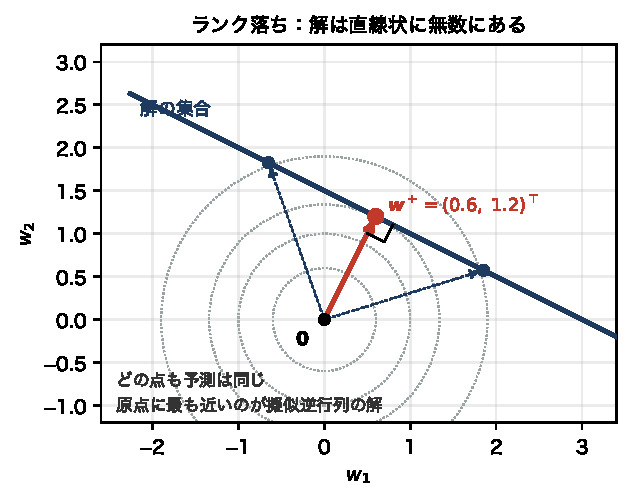
\includegraphics[width=0.60\linewidth]{figures/ch4_pseudoinverse}
  \caption{ランクが落ちた場合の解。直線上のどの点も同じ予測を与え、経験損失も等しい。
  擬似逆行列が選ぶのは、このうち原点に最も近い点（最小ノルム解）である。}
  \label{fig:pseudoinverse}
\end{figure}

\subsubsection{どれを選ぶか：最小ノルム解}

解が無数にあるとき、「正しい答え」は原理的に決まらない。
どれを選んでも訓練データへの当てはまりは同じだからである。
そこで\textbf{追加の基準}を持ち込む。最も標準的なのが
「解の中で、\textbf{パラメータベクトル $\bm{w}$ のノルム $\|\bm{w}\|$ が最小のもの}を選ぶ」という基準である。
ここでのノルムは誤差 $\|\bm{y} - \bm{X}\bm{w}\|$ のことではない。
誤差はどの解でも同じ最小値なので、それでは選べない。
比べるのは解そのもの、すなわち係数を並べたベクトル $\bm{w} = (w_0, w_1, \ldots, w_d)^\top$ の長さであり、
「係数の値が全体として小さい解を選ぶ」という意味である。
この「$\|\bm{w}\|$ を小さく保つ」という発想は、第6回のリッジ回帰（正則化）と同じものである。
両者の関係は第4.7.5項で述べる。

\begin{itembox}[l]{定義：ムーア・ペンローズ擬似逆行列}
任意の行列 $\bm{X} \in \mathbb{R}^{N \times (d+1)}$ に対して、
次の性質をもつ行列 $\bm{X}^{+} \in \mathbb{R}^{(d+1) \times N}$ がただ一つ存在する。
\begin{equation}
  \bm{w}^{+} = \bm{X}^{+}\bm{y}
  \label{eq:pinv-def}
\end{equation}
は、$\|\bm{y} - \bm{X}\bm{w}\|$ を最小にする $\bm{w}$ のうちで
$\|\bm{w}\|$ が最小のものである。
この $\bm{X}^{+}$ を\textbf{ムーア・ペンローズ擬似逆行列}
（Moore--Penrose pseudo-inverse）と呼ぶ。
\end{itembox}

「最小ノルム」という条件には幾何学的な意味がある。
解の集合\eqref{eq:solution-set}は、零空間を $\bm{w}^*$ だけ平行移動した集合である。
そのうち原点に最も近い点は、\textbf{零空間と直交する}点にほかならない
（図\ref{fig:pseudoinverse}）。
ここでも直交性が最適性を特徴づけている。本章で3度目である。

なお $\bm{X}^{+}$ は、次の4条件（ペンローズ条件）を満たす唯一の行列として定義することもある。
\begin{equation*}
  \bm{X}\bm{X}^{+}\bm{X} = \bm{X}, \quad
  \bm{X}^{+}\bm{X}\bm{X}^{+} = \bm{X}^{+}, \quad
  (\bm{X}\bm{X}^{+})^\top = \bm{X}\bm{X}^{+}, \quad
  (\bm{X}^{+}\bm{X})^\top = \bm{X}^{+}\bm{X}
\end{equation*}
第1式と第2式は逆行列の性質 $\bm{A}\bm{A}^{-1}\bm{A} = \bm{A}$ の緩和版であり、
第3式と第4式は $\bm{X}\bm{X}^{+}$ と $\bm{X}^{+}\bm{X}$ が射影行列であることを要求している。

\subsubsection{フルランクのときは何が起こるか}

$\bm{X}$ がフルランクなら零空間は $\{\bm{0}\}$ なので解は一つしかなく、
「最小ノルムのものを選ぶ」という条件は何も制限しない。
このとき擬似逆行列は具体的に書き下せる：
\begin{equation}
  \bm{X}^{+} = (\bm{X}^\top\bm{X})^{-1}\bm{X}^\top
  \label{eq:pinv-fullrank}
\end{equation}

式\eqref{eq:pinv-fullrank}は、擬似逆行列の定義（式\eqref{eq:pinv-def}）から次のように導かれる。
定義により $\bm{X}^{+}\bm{y} = \bm{w}^{+}$ であり、$\bm{w}^{+}$ とは
「$\|\bm{y} - \bm{X}\bm{w}\|$ を最小にする $\bm{w}$ のうち $\|\bm{w}\|$ が最小のもの」であった。
$\bm{X}$ がフルランクのとき、$\|\bm{y} - \bm{X}\bm{w}\|$ を最小にする $\bm{w}$ は
式\eqref{eq:ls-solution}の $\bm{w}^* = (\bm{X}^\top\bm{X})^{-1}\bm{X}^\top\bm{y}$ ただ一つである（第4.5.3項）。
候補が一つしかないのだから、その中でノルム最小のものも $\bm{w}^*$ 自身、すなわち $\bm{w}^{+} = \bm{w}^*$ である。
したがって
\begin{equation*}
  \bm{X}^{+}\bm{y} = \bm{w}^{+} = \bm{w}^* = (\bm{X}^\top\bm{X})^{-1}\bm{X}^\top\bm{y}
\end{equation*}
がどんな $\bm{y}$ に対しても成り立つ
（1つ目の等号は定義\eqref{eq:pinv-def}、2つ目はフルランクによる一意性、3つ目は式\eqref{eq:ls-solution}）。
$\bm{y}$ は任意なので、これは行列として $\bm{X}^{+} = (\bm{X}^\top\bm{X})^{-1}\bm{X}^\top$ ということである。

ペンローズ条件の側から確かめることもできる。
$\bm{P} = (\bm{X}^\top\bm{X})^{-1}\bm{X}^\top$ とおくと
$\bm{P}\bm{X} = (\bm{X}^\top\bm{X})^{-1}\bm{X}^\top\bm{X} = \bm{I}$ なので、
第1式 $\bm{X}\bm{P}\bm{X} = \bm{X}\bm{I} = \bm{X}$、
第2式 $\bm{P}\bm{X}\bm{P} = \bm{I}\bm{P} = \bm{P}$、
第4式 $(\bm{P}\bm{X})^\top = \bm{I}^\top = \bm{I} = \bm{P}\bm{X}$ が成り立つ。
第3式は $\bm{X}\bm{P} = \bm{X}(\bm{X}^\top\bm{X})^{-1}\bm{X}^\top = \bm{H}$ がハット行列であり、
その対称性は第4.6.2項で示した。
4条件を満たす行列は唯一なので、やはり $\bm{X}^{+} = \bm{P}$ である。

いずれにせよ式\eqref{eq:pinv-fullrank}は式\eqref{eq:ls-solution}と一致する。
つまり擬似逆行列は、\textbf{これまでの話を特別な場合として含む一般化}である。

さらに $\bm{X}$ が正方かつ正則なら $\bm{X}^{+} = \bm{X}^{-1}$ となる。
記号 $\bm{X}^{+}$ は $\bm{X}^{-1}$ の拡張だと思ってよい。

\subsubsection{数値例}

第3回の演習問題9で扱った行列を使う。
\begin{equation*}
  \bm{X} = \begin{pmatrix} 1 & 2 \\ 2 & 4 \end{pmatrix}, \qquad
  \bm{y} = \begin{pmatrix} 3 \\ 6 \end{pmatrix}
\end{equation*}
ここでは説明のためバイアス項を省き、2つの特徴だけを考えている。
第2列は第1列の $2$ 倍なので $\mathrm{rank}(\bm{X}) = 1$ であり、ランクが落ちている。

$\bm{y} = 3\,\bm{c}_1$ なので $\bm{y} \in \mathrm{Col}(\bm{X})$ であり、
誤差を $0$ にできる。条件は
\begin{equation*}
  w_1 + 2w_2 = 3
\end{equation*}
という1本の式だけで、これを満たす $(w_1, w_2)$ は直線上に無数にある。

零空間は $\bm{X}\bm{v} = \bm{0}$ すなわち $v_1 + 2v_2 = 0$ の解で、
$\bm{v} = (-2, 1)^\top$ の定数倍である。

最小ノルム解を求めよう。$w_1 = 3 - 2w_2$ を代入して
\begin{equation*}
  \|\bm{w}\|^2 = (3 - 2w_2)^2 + w_2^2 = 5w_2^2 - 12w_2 + 9
\end{equation*}
これを $w_2$ で微分して $0$ とおくと $10w_2 - 12 = 0$、すなわち $w_2 = 1.2$、$w_1 = 0.6$。
\begin{equation*}
  \bm{w}^{+} = \bm{X}^{+}\bm{y} = (0.6,\; 1.2)^\top, \qquad \|\bm{w}^{+}\| = \sqrt{1.8} \approx 1.342
\end{equation*}
これが零空間と直交することも確かめられる：
$\bm{w}^{+\top}\bm{v} = 0.6 \cdot (-2) + 1.2 \cdot 1 = 0$。

比べてみよう。$t = 1$ として $\bm{w}^{+} + \bm{v} = (-1.4,\; 2.2)^\top$ も解だが、
そのノルムは $\sqrt{1.96 + 4.84} \approx 2.608$ で、$\bm{w}^{+}$ より大きい。
予測はどちらも $\bm{X}\bm{w} = (3, 6)^\top$ で完全に同じである。

\subsubsection{なぜ最小ノルムを選ぶのか}

「どれも同じなら、なぜ小さいものを選ぶのか」という問いには、
第6回の正則化が答えを与える。

結論だけ先取りする。リッジ回帰は、経験損失に罰則 $\lambda\|\bm{w}\|^2$（$\lambda > 0$）を加えた
\begin{equation*}
  \|\bm{y} - \bm{X}\bm{w}\|^2 + \lambda\|\bm{w}\|^2
\end{equation*}
を最小にする。罰則の中身は、まさに本節で比べていた $\|\bm{w}\|$ である。
第4.3節と同じ手順で勾配を $\bm{0}$ とおくと（公式\eqref{eq:grad-quad}を $\lambda\bm{w}^\top\bm{I}\bm{w}$ にも使う）、
解は
\begin{equation*}
  \bm{w}_\lambda = (\bm{X}^\top\bm{X} + \lambda\bm{I})^{-1}\bm{X}^\top\bm{y}
\end{equation*}
となる。ここで $\bm{X}^\top\bm{X} + \lambda\bm{I}$ は、$\bm{X}$ がランク落ちしていても\textbf{つねに正則}である。
任意の $\bm{v} \neq \bm{0}$ に対して
$\bm{v}^\top(\bm{X}^\top\bm{X} + \lambda\bm{I})\bm{v} = \|\bm{X}\bm{v}\|^2 + \lambda\|\bm{v}\|^2 > 0$
となり、正定値だからである（第4.5.3項）。
つまり罰則を加えた瞬間に「解が無数にある」という問題は消え、解はつねに一意に定まる。
そして $\lambda$ を $0$ に近づけていくと、$\bm{w}_\lambda$ は\textbf{最小ノルム解 $\bm{w}^{+}$ に収束する}。
最小ノルム解は「ごくわずかに正則化した解」の極限なのである。

第3.6節で述べたとおり、重みが大きいと入力のわずかな違いが出力の大きな違いに増幅され、
ノイズを拾いやすくなる。同じ当てはまりなら重みは小さいほうがよい、というのは
汎化の観点から理にかなった選択なのである。


\subsection{数値計算上の注意}

理論的には $\bm{w}^* = (\bm{X}^\top\bm{X})^{-1}\bm{X}^\top\bm{y}$ で解ける。
しかし計算機でこの式をそのまま実装するのは\textbf{推奨されない}。

\subsubsection{条件数が二乗される}

行列の「解きにくさ」を測る量に\textbf{条件数}（condition number）がある。
対称かつ正定値な行列については、最大固有値と最小固有値の比
\begin{equation}
  \kappa(\bm{A}) = \frac{\lambda_{\max}(\bm{A})}{\lambda_{\min}(\bm{A})}
\end{equation}
で定義される。条件数が大きいほど、入力のわずかな誤差が解の大きな誤差に増幅される。
第3.7.3項で見た「細長い谷」は、まさに条件数が大きい状況であった。

ここで問題になるのは、$\bm{X}^\top\bm{X}$ を作った時点で
\begin{equation}
  \kappa(\bm{X}^\top\bm{X}) = \kappa(\bm{X})^2
\end{equation}
となり、条件数が\textbf{二乗されてしまう}ことである。
$\bm{X}$ の条件数が $10^4$ 程度でも、$\bm{X}^\top\bm{X}$ では $10^8$ になる。
倍精度計算の有効桁数がおよそ $16$ 桁であることを考えると、無視できない劣化である。

\subsubsection{実際に使われる方法}

そこで数値計算では、$\bm{X}^\top\bm{X}$ を明示的に作らずに解く方法が用いられる。
詳細は本講義の範囲を超えるが、考え方だけ述べておく。

\begin{itemize}
  \item \textbf{QR分解}：$\bm{X} = \bm{Q}\bm{R}$（$\bm{Q}$ は列が直交、$\bm{R}$ は上三角）と分解し、
    $\bm{R}\bm{w} = \bm{Q}^\top\bm{y}$ を解く。条件数が二乗されない。
  \item \textbf{特異値分解（SVD）}：$\bm{X}$ を3つの行列の積に分解する方法で、
    ランクが落ちていても扱える。擬似逆行列はこの分解を用いて計算される。
\end{itemize}

実装上は、自分で逆行列を書くのではなくライブラリの最小二乗ソルバを使うのが鉄則である。
Python では \verb|numpy.linalg.lstsq| がこれにあたり、内部ではSVDが使われる。
擬似逆行列そのものは \verb|numpy.linalg.pinv| で得られる。

\subsubsection{多重共線性との関係}

第3.5.5項で見た多重共線性は、ここでは条件数の問題として現れる。
特徴どうしが強く相関していると $\bm{X}$ の条件数が大きくなり、
$\bm{X}^\top\bm{X}$ の最小固有値が $0$ に近づく。
形式的には正則でも、数値的にはほとんど特異であり、解は信用できない。

対処は3つある。
\begin{enumerate}
  \item 相関の強い特徴を削る（特徴選択）
  \item 正則化を入れて $\bm{X}^\top\bm{X} + \lambda\bm{I}$ とする（第6回）
  \item 擬似逆行列を使い、最小ノルム解を取る
\end{enumerate}
2番目が実務で最もよく使われる。$\lambda\bm{I}$ を足すと最小固有値が $\lambda$ だけ持ち上がり、
条件数が改善するからである。この見方は第6回で詳しく扱う。


\subsection{まとめ}

\begin{itemize}
  \item 最小二乗法は「列空間の中で $\bm{y}$ に最も近い点を探す」問題であり、
    その答えは $\bm{y}$ の\textbf{正射影}である
  \item 最適性の条件は\textbf{誤差が列空間と直交すること}であり、
    これを式にしたものが\textbf{正規方程式} $\bm{X}^\top\bm{X}\bm{w} = \bm{X}^\top\bm{y}$ である
  \item 同じ式は $L_D$ を微分して $\nabla L_D = \bm{0}$ とおいても得られる。
    「勾配が $\bm{0}$」と「誤差が直交」は同じ条件である
  \item $\bm{X}^\top\bm{X}$ はつねに対称かつ半正定値。
    $\bm{X}$ がフルランクのときに限り正定値（＝正則）となり、解は
    $\bm{w}^* = (\bm{X}^\top\bm{X})^{-1}\bm{X}^\top\bm{y}$ と一意に定まる
  \item 予測は $\hat{\bm{y}} = \bm{H}\bm{y}$ と書け、ハット行列 $\bm{H}$ は
    対称・冪等であり $\mathrm{tr}(\bm{H}) = d+1$（モデルの自由度）である
  \item ランクが落ちると解は無数に存在する。
    \textbf{擬似逆行列} $\bm{X}^{+}$ はそのうち\textbf{ノルム最小}のものを選ぶ
  \item 計算機では $\bm{X}^\top\bm{X}$ を作らず、QR分解やSVDで解く。
    条件数が二乗されるのを避けるためである
\end{itemize}

本章では解を\textbf{閉じた式}で求めた。
しかしこの方法は、$d$ が非常に大きいとき（$\bm{X}^\top\bm{X}$ が巨大になる）や、
モデルが線形でないときには使えない。
次回（第5回）は、同じ最小化問題を\textbf{反復計算}で解く方法、
すなわち勾配降下法を扱う。
本章で定義した勾配 $\nabla L_D$ が、そこで主役になる。


\subsection{演習問題}

\begin{enumerate}

  \item \textbf{直交性の確認}\quad
    $\bm{X} = \begin{pmatrix} 1 & 0 \\ 1 & 1 \\ 1 & 2 \end{pmatrix}$、
    $\bm{y} = (1, 2, 2)^\top$ とする。
    \begin{enumerate}
      \item $\bm{X}^\top\bm{X}$ と $\bm{X}^\top\bm{y}$ を求めよ。
      \item 正規方程式を解いて $\bm{w}^*$ を求めよ。
      \item 残差 $\bm{r} = \bm{y} - \bm{X}\bm{w}^*$ を求め、
        $\bm{X}^\top\bm{r} = \bm{0}$ を確認せよ。
      \item 経験損失 $L_D(\bm{w}^*)$ を求めよ。
    \end{enumerate}

  \item \textbf{三平方の定理による最適性}\quad
    問1の設定で、$\bm{w} = (1, 1)^\top$ としたときの予測を $\bm{X}\bm{w}$ とする。
    \begin{enumerate}
      \item $\|\bm{y} - \bm{X}\bm{w}\|^2$ を計算せよ。
      \item $\|\bm{y} - \hat{\bm{y}}\|^2 + \|\hat{\bm{y}} - \bm{X}\bm{w}\|^2$ を計算し、
        (a) と一致することを確認せよ（式\eqref{eq:ch4-pythagoras}）。
      \item この等式が成り立つのはなぜか。どのベクトルとどのベクトルが
        直交していることを使っているか明記して説明せよ。
    \end{enumerate}

  \item \textbf{微分による導出}\quad
    $L_D(\bm{w}) = \frac{1}{N}\|\bm{y} - \bm{X}\bm{w}\|^2$ について答えよ。
    \begin{enumerate}
      \item $N \cdot L_D(\bm{w})$ を展開し、式\eqref{eq:ch4-expand}の形に書け。
        途中で使った「スカラーの転置は変わらない」という事実がどこで効いたか示せ。
      \item 公式\eqref{eq:grad-linear}と\eqref{eq:grad-quad}を用いて $\nabla L_D$ を求めよ。
      \item $\nabla L_D = \bm{0}$ から正規方程式を導け。
    \end{enumerate}

  \item \textbf{行列微分の公式}\quad
    $\bm{A} \in \mathbb{R}^{p \times p}$ を\textbf{対称とは限らない}定行列とする。
    \begin{enumerate}
      \item $\nabla_{\bm{w}}(\bm{w}^\top\bm{A}\bm{w}) = (\bm{A} + \bm{A}^\top)\bm{w}$
        を成分計算で示せ。
      \item $\bm{A}$ が対称のとき、これが $2\bm{A}\bm{w}$ になることを確認せよ。
      \item $\bm{A} = \begin{pmatrix} 1 & 2 \\ 0 & 3 \end{pmatrix}$、
        $\bm{w} = (w_1, w_2)^\top$ のとき、
        $\bm{w}^\top\bm{A}\bm{w}$ を $w_1, w_2$ の式として書き下し、
        偏微分して (a) の結果と一致することを確かめよ。
    \end{enumerate}

  \item \textbf{ハット行列}\quad
    問1の $\bm{X}$ について答えよ。
    \begin{enumerate}
      \item $\bm{H} = \bm{X}(\bm{X}^\top\bm{X})^{-1}\bm{X}^\top$ を計算せよ。
      \item $\bm{H}^\top = \bm{H}$ と $\bm{H}^2 = \bm{H}$ を確認せよ。
      \item $\mathrm{tr}(\bm{H})$ を求め、$d+1$ に一致することを確認せよ。
      \item $\bm{H}$ の固有値は $0$ か $1$ のいずれかであることを、
        $\bm{H}^2 = \bm{H}$ から示せ。固有値 $1$ の個数は何個か。
    \end{enumerate}

  \item \textbf{一意可解性}\quad
    \begin{enumerate}
      \item 任意の $\bm{v}$ に対して $\bm{v}^\top\bm{X}^\top\bm{X}\bm{v} = \|\bm{X}\bm{v}\|^2$
        が成り立つことを示せ。
      \item これを用いて、$\bm{X}$ の列が線形独立ならば $\bm{X}^\top\bm{X}$ が
        正定値であることを示せ。
      \item 逆に、$\bm{X}$ の列が線形従属ならば $\bm{X}^\top\bm{X}$ は正則でないことを示せ。
      \item $N = 5$, $d = 10$（特徴が10個）のとき、$\bm{X}^\top\bm{X}$ は正則になりうるか。
        理由とともに述べよ。
    \end{enumerate}

  \item \textbf{擬似逆行列}\quad
    $\bm{X} = \begin{pmatrix} 1 & 3 \\ 2 & 6 \end{pmatrix}$、
    $\bm{y} = (2, 4)^\top$ とする。
    \begin{enumerate}
      \item $\mathrm{rank}(\bm{X})$ を求めよ。
      \item $\mathrm{Null}(\bm{X})$ を求めよ。
      \item $\|\bm{y} - \bm{X}\bm{w}\|$ を最小にする $\bm{w}$ の集合を書き下せ。
      \item そのうちノルム最小のもの $\bm{w}^{+}$ を求めよ。
      \item $\bm{w}^{+}$ が $\mathrm{Null}(\bm{X})$ と直交することを確認せよ。
    \end{enumerate}

  \item \textbf{条件数}\quad
    $\bm{X}^\top\bm{X} = \begin{pmatrix} 1 & 0 \\ 0 & \varepsilon \end{pmatrix}$
    （$\varepsilon > 0$ は小さい数）という状況を考える。
    \begin{enumerate}
      \item 固有値と条件数 $\kappa(\bm{X}^\top\bm{X})$ を求めよ。
      \item $\bm{X}^\top\bm{y} = (1, \varepsilon)^\top$ のとき $\bm{w}^*$ を求めよ。
      \item $\bm{X}^\top\bm{y}$ の第2成分が $\varepsilon$ から $2\varepsilon$ に変化したとき、
        $\bm{w}^*$ はどれだけ変化するか。$\varepsilon$ が小さいほど
        何が問題になるか説明せよ。
      \item $\bm{X}^\top\bm{X} + \lambda\bm{I}_2$（$\lambda > 0$）としたとき、
        条件数はどうなるか。$\lambda$ を大きくすると条件数はどう変わるか。
    \end{enumerate}

\end{enumerate}


\end{document}



























